%!TEX encoding = UTF-8 Unicode
\documentclass[12pt,a4paper,papersize,oneside]{jsbook}

\usepackage[T1]{fontenc}
\usepackage{amsmath}
\usepackage{amssymb}
\usepackage{stix} % math font: STIX font
%\usepackage{newtxmath} % math font: Times like
%\usepackage{newpxmath} % math font: Platino like
%\usepackage{eulervm} % math font: hand write like
%\usepackage{newtxtext} % text font: Times like
\usepackage{newpxtext} % text font: Platino like
\usepackage[dvipdfmx]{graphicx}
\graphicspath{{Fig/}}
\usepackage{url}
\usepackage[dvipdfmx]{hyperref}
\usepackage[dvipdfmx]{pxjahyper} % 日本語のhyperref
\usepackage{makeidx}\makeindex  % allows for indexgeneration

\usepackage[bold]{otf}
\usepackage{pifont}
\usepackage{array,booktabs}
\usepackage{setspace}
\usepackage{enumitem}
\usepackage{subcaption}

% PDF meta information and bookmarks
\hypersetup{
bookmarks=true,         % show bookmarks bar?
bookmarksnumbered=true,
bookmarkstype=toc,
%unicode=true,          % non-Latin characters in Acrobat’s bookmarks
pdftoolbar=true,        % show Acrobat’s toolbar?
pdfmenubar=true,        % show Acrobat’s menu?
pdffitwindow=false,     % window fit to page when opened
pdftitle={推薦システムのアルゴリズム},    % title
pdfauthor={神嶌 敏弘},     % author
pdfsubject={}, % subject
pdfkeywords={推薦システム;recommender system;協調フィルタリング;collaborative filtering}, % list of keywords
pdfnewwindow=true,      % links in new window
%setpagesize=false, % setting paper size
}

% local macro definitions
\usepackage{mathsymbols}
\usepackage{myindex}

% set pagesize: A4paper, margin=3cm
\setlength{\topmargin}{4.6truemm}
\setlength{\headheight}{1\baselineskip}
\setlength{\headsep}{1\baselineskip}
\setlength{\textheight}{\paperheight}\addtolength{\textheight}{-60truemm}\addtolength{\textheight}{-2\baselineskip}
\setlength{\footskip}{0pt}
\setlength{\oddsidemargin}{4.6truemm}
\setlength{\evensidemargin}{\oddsidemargin}
\setlength{\textwidth}{\paperwidth}\addtolength{\textwidth}{-60truemm}
\setlength{\fullwidth}{\textwidth}

%%%% more linebreaks in equations %%%%

\binoppenalty=0
\relpenalty=0
% \mathcode`\,="202C      % "," is considered as a binary operator

%%%%% condense floats %%%%%

%\def\topfraction{0.99}
%\def\bottomfraction{0.01}
%\def\textfraction{0.01}
%\def\floatpagefraction{0.99}
%\def\dbltopfraction{0.99}
%\def\dblfloatpagefraction{0.99}

%%%%% title, author, and release %%%%%

\title{\Huge\sffamily\bfseries 推薦システムのアルゴリズム}
\author{\Large\textbf{神嶌 敏弘} \quad$\langle\,$\url{http://www.kamishima.net/}$\,\rangle$}
\date{Release: \input{version}}

\begin{document}

% ===== Front Matter =====
\frontmatter

% --- Title ---
\maketitle

% --- Preface & Notation---
\onehalfspacing

%!TEX root =  main.tex
%!TEX encoding = UTF-8 Unicode
\chapter*{まえがき}
\label{chap:preface}

本稿は推薦システムについてまとめたものである.

人工知能学会誌2007年11月号~\cite{jpublist:076},2008年1月号~\cite{jpublist:081},および2008年3月号~\cite{jpublist:083}の3回に渡って連載した解説記事「推薦システムのアルゴリズム(1)〜(3)」に対し,誤りの訂正や,新しい内容の追加などの更新を行ったものである.

本稿のソースファイルは \texttt{GitHub} にて公開している.
\begin{quote}
\url{https://github.com/tkamishima/recsysdoc}
\end{quote}
TYPOや記述の誤りなどのバグリポートは,\texttt{GitHub} の rull request か,issues を使って連絡されたい.
なお,事情によりすぐには対処できない場合があるので,予めご了解いただきたい.

\section*{本稿の構成}
\label{sec:preface-organization}

本稿の構成は以下のとおりである.
第\ref{part:overview}部では,推薦システムとは何か,またその設計指針や分類について述べる.
第\ref{part:process}部では,データの入力,嗜好の予測,そして推薦の提示からなる推薦システムの実行過程について述べる.
第\ref{part:algoirthm}部では,さまざまな嗜好の予測アルゴリズムのを紹介する.
第\ref{part:topic}部では,推薦システムに関連する話題や,さまざまな状況での推薦を紹介する.
第\ref{part:conclusion}部は関連資料の紹介とまとめである.

%!TEX root =  main.tex
%!TEX encoding = UTF-8 Unicode
\chapter*{謝辞}
\label{chap:ack}

チュートリアル記事の執筆にあたり以下の方々の協力を得たことに感謝する.
麻生英樹,岩田具治,佐藤健,廣瀬勝一,藤井敦,村上知子,山口高平には,本稿に関する貴重なコメントをいただいた.
J.~Riedl,J.~Herlockerには論文の詳細について教えていただいた.
アマゾンジャパン様,アップルジャパン様,GroupLensプロジェクト様にはWWWのスクリーンショットなどの掲載を許可いただいた.

本稿の更新に関して次の方々の協力を得たことに感謝する:
赤穂昭太郎,石黒勝彦,岡野原大輔,奧健太,折田明子,酒井哲也,佐久間淳,佐藤一誠,冨岡亮太,中川裕志,土方嘉徳,星野伸明

%!TEX root =  main.tex
%!TEX encoding = UTF-8 Unicode
\chapter*{数式の表記}
\label{chap:notation}

スカラーの変数はイタリック体 $x$ で,一部の確立変数は大文字のイタリック体 $X$,ベクトルは小文字ボールド体 $\bfx$で,行列は大文字ボールド体 $\bfX$で表記する.
実数などの特殊なものを除き,集合にはカリグラフィック体 $\calD$ を用いる.

\begin{center}
\small\renewcommand{\arraystretch}{0.8}
\begin{tabular}{@{}>{\centering}p{0.09\fullwidth}@{\hspace{0.01\fullwidth}}p{0.38\fullwidth}@{\hspace{0.04\fullwidth}}>{\centering}p{0.09\fullwidth}@{\hspace{0.01\fullwidth}}p{0.38\textwidth}@{}}\toprule
\textbf{表記} & \textbf{意味} & \textbf{表記} & \textbf{意味} \\ \cmidrule(r){1-2}\cmidrule{3-4}
$x$ & 特定の利用者を表す & $y$ & 特定のアイテムを表す \\
$X$ & 利用者を表す確率変数 & $Y$ & アイテムを表す確率変数 \\
$\bfx$ & 利用者をまとめたベクトル & $\bfy$ & アイテムをまとめたベクトル \\
$n$ & 利用者数 & $m$ & アイテム数 \\
$\calX$ & 利用者集合 $\{1,\ldots,n\}$ & $\calY$ & アイテム集合 $\{1,\ldots,m\}$ \\
$\calX_y$ & アイテム$y$を評価した利用者の集合 & $\calY_x$ & 利用者xが評価したアイテムの集合 \\
$a$ & 活動利用者を表す & $r_{xy}$ & 利用者$x$のアイテム$y$への評価値 \\
$\bar{r}_x$ & 利用者$x$による評価値の平均 & $\tilde{r}_y$ & アイテム$y$への評価値の平均 \\
$\bfR$ & 評価値行列 & $\calR$ & 評価値集合(5段階評価なら $\{1,\ldots,5\}$) \\
$\bfr$ & 評価値をまとめたベクトル & $z$ & 潜在因子 \\
$\bfz$ & 潜在因子のベクトル & $K$ & 潜在因子の数・次元数 \\
$\calD$ & データ集合 & $N$ & 訓練データ数 \\
$\bfU$ & 利用者潜在因子行列 & $\bfV$ & アイテム潜在因子行列 \\
$\bfu_{x}$ & 利用者$x$の潜在因子ベクトル & $\bfv_{y}$ & アイテム$y$の潜在因子ベクトル \\
$y^{(t)}$ & 時刻$t$での値 & $\ang{Y^{(t)}}$ & アイテムの時系列 \\
$\theta\,\bftheta\,\bfTheta$ & パラメータを一般に表す & $\sig()$ & シグモイド関数 \\
$\Dom()$ & 変数の定義域 & $\nan$ & 欠損値 \\
\bottomrule
\end{tabular}
\end{center}

スカラー関数 $f(x)$ に対して,その引数をベクトルとする表記 $f(\bfx)$ は,ベクトル $\bfx$ の各要素を関数 $f$ に適用して得られるベクトルを表す.

確率変数 $X$ が離散の場合の確率質量関数も,連続値の場合の確率密度関数も特に区別することなく $\pb{X}$ と表記する.

$\expect_{\pb[X]}[f(X)]$ は,分布 $\pb{X}$ についての次の期待値を表す:
\[
\begin{array}{l@{\text{ \makebox[3zw]{\dotfill} }}l}
\sum_{x\in\Dom(X)} f(x) \pb{X=x} & \text{$X$が離散の場合}\\
\int_{x\in\Dom(X)}  f(x) \pb{X=x} dx & \text{$X$が連続の場合}
\end{array}
\]
なお,$\pb{X}$を省略した場合は,関数$f$の全ての確率変数の同時分布に関する期待値を表す.例えば,$\expect[f(X,Y)]$ は,$\expect_{\pb{X,Y}}[f(X,Y)]$ の意味である.


% --- Table of Contents ---
\tableofcontents

% ===== Main Matter =====
\mainmatter

% ---- Main Content ----

\part{推薦システムの概要}
\label{part:overview}
%!TEX root =  main.tex
%!TEX encoding = UTF-8 Unicode
\chapter{推薦システム}
\label{chap:intro}

「\term{推薦システム}{recommender system}」とは,利用者にとって有用と思われる対象,情報,または商品などを選び出し,それらを利用者の目的に合わせた形で提示するシステムである.

最初に,この推薦システムが必要になった背景について述べよう.
第一に,大量の情報が発信されるようになったことがある.
これは,情報化技術の進展により,個人・団体が容易かつ低コストで発信できるようになったためである.
第二の理由は,これら大量の情報の蓄積や流通が容易になり,誰もが大量の情報を得ることができるようになったことである.
これも計算機の記憶媒体の大規模化や,通信の高速化によるものである.
以上のことから,大量に発信された情報を,だれもが大量に取得できる状況が生じた.
しかし,欲しい情報が何か分からない(例:統計資料として公開されているがその名前が分からない)とか,探している情報を見つけ出せない(例:類似した資料が大量にあり目的のものが埋もれてしまう)といった理由により,情報を参照できる状態にあるにもかかわらず,それを利用できないという状況が生じた.
この状況を「\term{情報過多}{information overload}~\cite{misc:009}
\footnote{情報爆発 (information explosion) や情報洪水 (information overflow) ともいう.}
という.
この状況を打破するため,利用者にとって有用な情報を見つけ出す推薦システムが考案された.

この推薦システムは,広い立場からみれば,情報検索や情報フィルタリング技術の一つと見なせる.そのため,初期の推薦システムは,これらの技術が基盤となっていた.
\ref{chap:process}章で述べるように,このシステムの実現手法には協調フィルタリングと内容ベースフィルタリングがある.
だが,協調フィルタリングという語の方が推薦システムより古く,1992年に文献 \cite{macm:92:01} にて使われた.
だが,これは現在のような協調フィルタリングではなく,他人が手動で行った推薦を検索できる協調作業支援のシステムであった.
この過程を自動化した協調フィルタリングが1994年のGroupLens\cite{cscw:94:01}やRingo \cite{sigchi:95:02}であり,現在の推薦システムの基礎となった.
一方の内容ベースフィルタリングの技術は,従来からある情報フィルタリングとみなせ,また,事例ベース推論の応用としても研究されてきた.
そのうち,推薦システムとして独自の側面が強くなり,協調フィルタリングに対して内容ベースフィルタリングと呼ばれるようになった.
1996年には,専門のワークショップも開催されるほどに研究が活発化した.
1997年にはACM Communications誌で特集\cite{macm:97:01} が掲載され,この種のシステムの呼び名として「Recommender System」が定着した.
このころから,NetPerceptions や Firefly などの企業によってシステムの商業化が始まった.
現在では,Webを通じた各種サービスの機能で活用されたり\cite{ieeem:99:02,ieeem:03:01,www:07:01},セットトップボックスなど
の機器に組み込まれたり\cite{kdd:04:11}している.
その後,物理的な店舗面積に商品数が制限されない電子商取引の発展や,大量の画一的な商品から,少量多品種への消費傾向の変化にに伴って,その重要性も広く認識されるようになった.
それを象徴する Amazon.com CEOのJeff Bezosの発言を引用しておこう\cite{dmkd:01:01}%
\footnote{J.~Riedlのメールによれば,J.~Bezosは,この発言を幾つかの講演で行った.ここでは,300万人と書いたが,そのときどきの顧客数に応じて,この数字は変えて用いられた.} .
\begin{center}
\cornersize*{2zw}\setlength{\fboxsep}{1zw}
\ovalbox{\begin{minipage}{0.92\linewidth}
\large\itshape
If I have 3 million customers on the Web,\\
\hfill{}I should have 3 million stores on the Web

\small\rmfamily\centering
(Webに3百万人の顧客がいるなら,3百万のWebストアを用意すべきだ)
\end{minipage}}
\end{center}
現在では,推薦システムは多方面で利用され,研究も継続的に行われ,多様な方法が目的に応じて考案されている.
これらの推薦システムの設計指針やアルゴリズムについてまとめる.

%!TEX root =  main.tex
%!TEX encoding = UTF-8 Unicode
\chapter{推薦システムの分類と目的}
\label{sec:rsysgoal}

本節では,推薦の個人化の度合いの分類と,運用側と利用者側のそれぞれ目的によるシステムの分類について述べる.
これらの目的を考慮して,推薦システムの設計方針を決めることになる.

その前に,推薦システムに関連する技術と,それらとの違いについて述べておく.
まず,情報検索における情報フィルタリングがある.これは,逐次的に入力される情報から,利用者の関心や興味を記述した利用者プロファイルに適合するものを選別する技術\cite{jb:012:00}で,推薦システムと良く似ている.
だが,主にテキスト文書を扱い,利用者プロファイルも主に索引語で示す点や,必要なものを取り出すより,不要なものを除外することが主目的である点などがが異なる.
他に,マーケティングの技術とも関連がある.
しかし,マーケティングが供給側の視点に立つのに対し,推薦システムは消費側である.推薦システムの推薦が利用者に受け入れられるためには,推薦が実際に客観的なものであり,また,そのことを利用者に示す工夫が必要になる.
また,マーケティングでは,レポートなど全体の傾向などを分析して報告することが必要だが,推薦システムにはそうしたことは要求されない.
また,マーケティングでは,顧客を客層に分類し,それに応じた対処を行うが,推薦システムでは,利用者のグループ化は目的ではない.

\section{推薦の個人化の度合い}
\label{sec:plevel}

最初に,推薦の個人化の度合いの3段階\cite{dmkd:01:01}を示す.

\begin{figure}
\centering
\begin{minipage}{0.45\fullwidth}
\centering
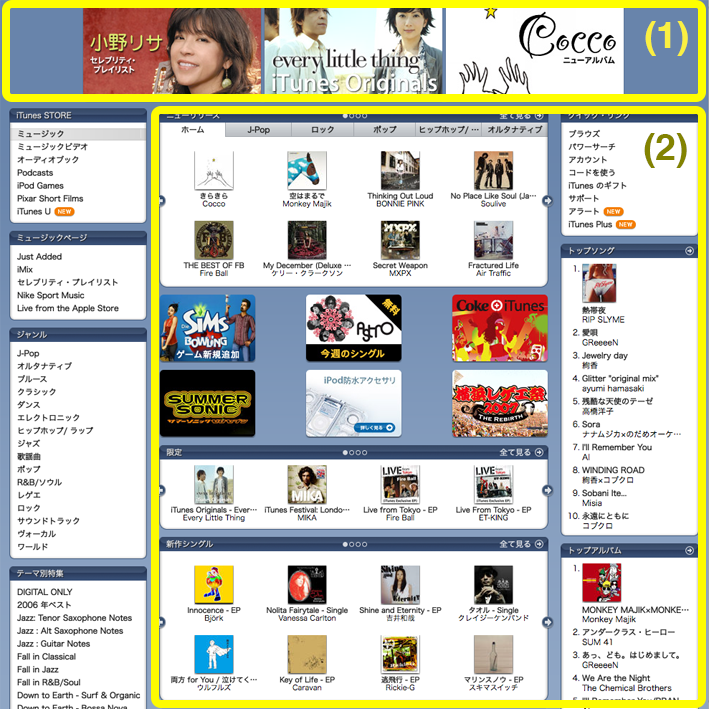
\includegraphics[width=\textwidth]{example1.png}\\
(a)~非個人化 (iTunes Store)
\end{minipage}
\hspace{0.02\fullwidth}
\begin{minipage}{0.45\fullwidth}
\centering
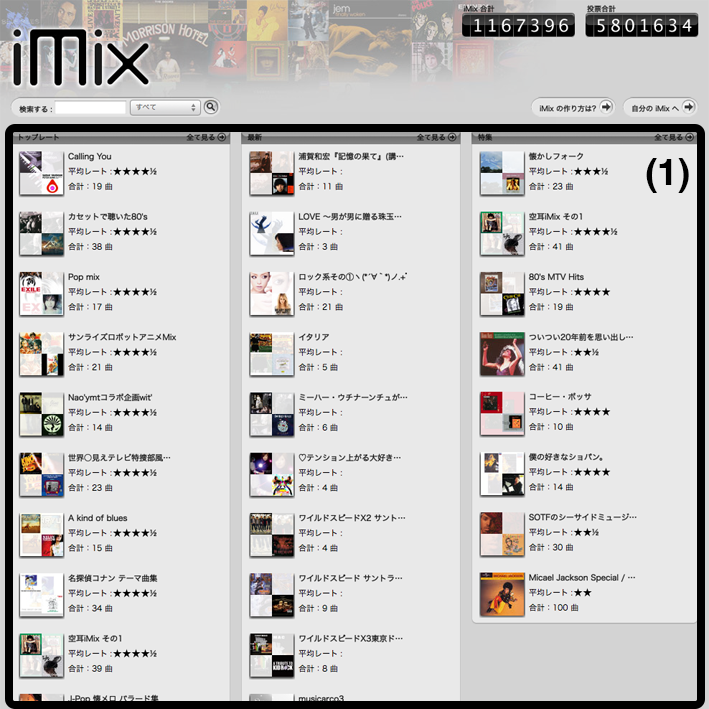
\includegraphics[width=\textwidth]{example2.png}\\
(b)~非個人化 (iTunes Store)
\end{minipage}
\medskip\\
\begin{minipage}[b]{0.45\fullwidth}
\centering
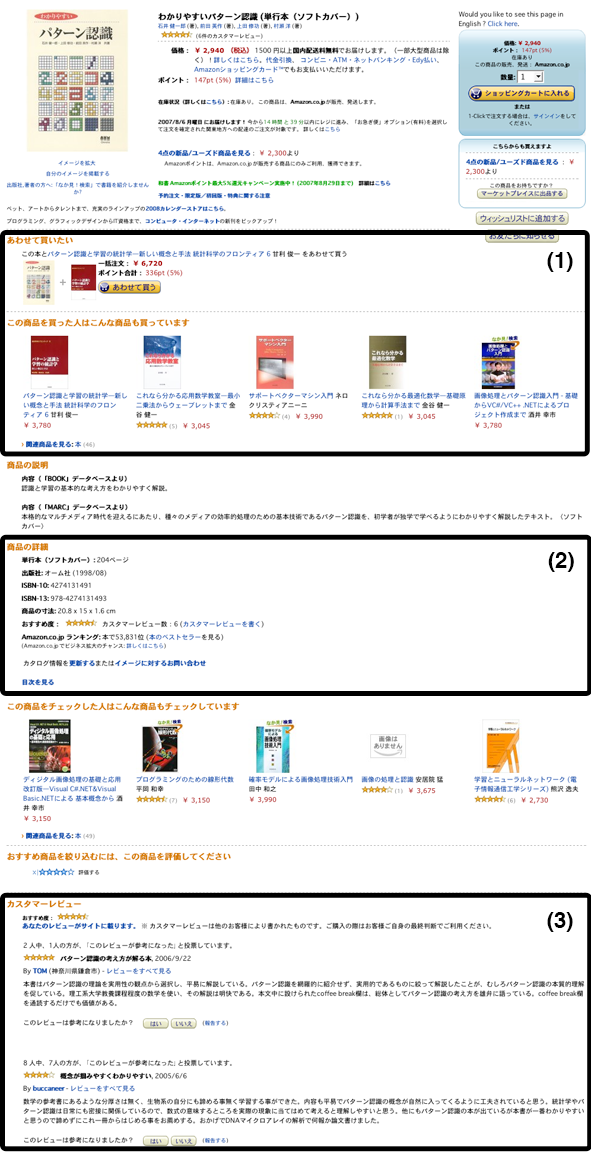
\includegraphics[width=\textwidth]{example56.png}\\
(c)~一時的個人化 (Amazon.co.jp)
\end{minipage}
\hspace{0.02\fullwidth}
\begin{minipage}[b]{0.45\fullwidth}
\centering
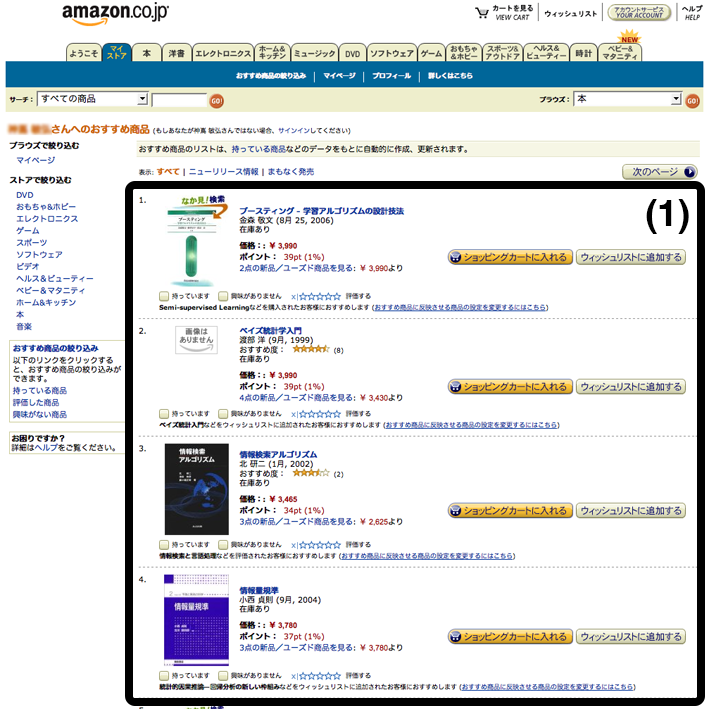
\includegraphics[width=\textwidth]{example4.png}\\
(d)~永続的個人化 (Amazon.co.jp)
\end{minipage}
\bigskip\\
\caption{個人化の度合いの異なる推薦の例}
\label{fig:plevel}
{\footnotesize 図(a),(b),(d) は2007/07/26日に,図(c)は2007/08/04日にスクリーンショットを取得した.}
\end{figure}

\begin{description}[style=nextline]
\item[\term{非個人化}{no personalization}]
全ての利用者について,全く同じ推薦をする場合である.
例えば,編集者による推薦や,売り上げ順位リストなどである.
推薦システムというときは個人化かつ自動化されたものを想定するかもしれないが,こうしたものも広義には含める.
非個人化の推薦の例を図\ref{fig:plevel}(a)と(b)に示す.
図\ref{fig:plevel}(a)中の,(1)は店舗の編集者が手作業で選んだもの,(2)は予約や売り上げの順位リストである.
システム側だけでなく,図\ref{fig:plevel}(b)のように,他の利用者が手作業で作成する推薦リストもある.
\item[\term{一時的個人化}{ephemeral personalization}]
システムを利用する一つのセッションで同じ入力や振る舞いをした利用者には,同じ推薦をする場合である.
一時的個人化の推薦の例を図\ref{fig:plevel}(c)に示す.
この例では,利用者がある本を閲覧するという行動をシステムに対してしたとき,その本に関連する情報を示している.
図中の,(1)はこの本と関連が深い本を推薦し,(2)には,書誌情報や売り上げ順位など,(3)では他の利用者の評価やコメントなど,この本についての関連情報を提示している.
\item[\term{永続的個人化}{persistent personalization}]
たとえ同じ入力や行動をシステムにしている利用者でも,利用者の個人情報や過去の利用履歴に応じて異なる推薦をする場合である.
例えば,過去の購入・利用履歴に基づいて推薦したり,年齢に応じて推薦するアイテムを変えたりする.
永続的個人化の推薦の例である図\ref{fig:plevel}(d)では,この利用者の過去の商品への評価に基づいて,関心があるであろう本を予測し,順位付けして提示している.
\end{description}

\section{推薦システムの運用目的の分類}
\label{sec:systemtarget}

次に,推薦システムを,運用側の目的に基づいて分類する.
文献\cite{dmkd:01:01}では,自動・手動の推薦システムを次の5種類に分
類し,目的に応じて適切に組み合わせて利用すべきと述べている.

\begin{description}[style=nextline]
\item[概要推薦 (broad recommendation)]
これは,全体の統計情報や運用者側の編集者を使う場合である.
全体の統計情報とは「今週の売り上げランキング」や「個々の商品の売り上げ順位」といったもので,編集者による推薦には「評論家が推薦する映画」や「特売品リスト」などがある.
図\ref{fig:plevel}(a)はこうした概要推薦の例である.
こうした概要推薦は,システムを利用し始めたばかりか,ごくまれにしか利用しないような利用者を対象とする.
これらの利用者が,自身の要求との関連性を見いだして,システムの利用を続けてもらえるように,大まかな情報を提供するのが目的である.
よって,積極的に探さなくても見えるように,システムにアクセスしたとき最初に見える場所に配置するべき推薦である.
加えて,利用者が積極的にシステムに働きかけることは期待できないので,非個人化または,アイテムのカテゴリを示す程度の入力に対応した一時的個人化した推薦をすべきである.
\item[利用者評価 (user comments and rating)]
これは,運用側が用意したシステム上で,利用者間での推薦をする場合である.
例えば,読者の批評文や★の数で示した評価レートをつけられるようにし,それらを他の利用者が参照したり,平均評価値などの統計情報を見たりできるようにする.
図\ref{fig:plevel}(b)のような他の利用者による推薦リストや,図\ref{fig:plevel}(c)の(3)のように他の利用者による評価やコメントなどが
この種の推薦の例である.\par
一般に,運用側のシステムが第三者的な立場で推薦しているとは,利用者にはあまり思われない.
それに対し,他の利用者の方がずっと信用され,その推薦も受け入れられやすい.
運用側には,システムに対する利用者の信頼を高めたり,利用頻度を高めたりといった利点がある.
こうした推薦は,運用側の関与は少なく,評価値順のアイテムリストなどの非個人化か,閲覧中のアイテムの評価値やコメントなどの単純な一時的個人化が行われる.
\item[通知サービス (notification service)]
これは,利用者がシステムを操作していないときに,電子メールなどで推薦を配送する場合である.
一つには,過去の購買履歴に基づいて,新規のアイテムの中から推薦リストを生成し,利用者に送付するといった,永続的個人化をするものがある.
また,利用者が予め設定した条件,例えば,ファンである歌手などを設定しておくと,その歌手の新譜の案内が届くという一時的個人化をした推薦もある.
これらの推薦は,システムの再利用を利用者に促すことを目的とする.
\item[関連アイテム推薦 (item-associated recommendation)]
利用者が注目している,例えば,電子商取引サイトで,商品を閲覧しているとか,「買い物かご」にすでに商品を入れている状況を想定する.
このとき,注目しているアイテムの比較候補(例:他メーカーの同等品)を示して,購入の判断を助けたり,購入の決断を促す場合や,補足的な商品などを提示してcross-selling(例:ハンバーガーにポテトなどの関連品を薦めて同時に購入させる)を促す場合がこの種の推薦である.
例としては,図\ref{fig:plevel}(c)の(1)のように閲覧中の商品の関連商品を示すものがある.
注目している商品の情報だけに基づく一時的個人化も,利用者の過去の行動も考慮する永続的個人化も可能である.
\item[緊密な個人化 (deep personalization)]
システムが積極的に利用者の情報を能動的に収集したり,過去の行動の情報を蓄積し,それらに基づいて推薦を行う場合である.
図\ref{fig:plevel}(d)のような,個人向けの推薦リストなどが,この種の推薦に該当する.
利用者がシステムを利用し続けることで蓄積された情報に基づいて,永続的な個人化が可能になる.すると,より適切な推薦ができるようになり,他のシステムとの差別化につながり,利用者の長期間にわたるロイヤリティ構築に役立つ.
だが,一方で,最も実装に困難が伴い,コストも要する.
\end{description}

\section{推薦システムの予測タスクの分類}
\label{sec:recomtask}

推薦システムが達成するタスクに基づく分類を文献\cite{jacm:04:01,jmlr:09:01}に沿って示す.

\begin{description}[style=nextline]
\item[\termmain{適合アイテム発見}{finding some good items}]
このタスクの目的は,利用者が自分の嗜好に適合するものを,何か見つけ出すことである.
利用者が積極的な動機を持って,情報を見つけるために推薦システムを利用するときは,こうした目的になる.\par
例えば,今から食べに行く店を決めるために,レストラン推薦システムを利用することが想定される.
この場合には,予測される評価の高い,比較的少数のものに絞り込んで利用者に提示する.
利用者はこのリストを上位から閲覧することで,自身の決定に必要な情報を知ることができるだろう.
\item[\termmain{評価値予測}{predicting ratings}]
このタスクの目的は利用者がアイテムに付けるであろう評価値を予測することである.
何らかのフォーマットに従ってアイテムが整列されていたり,構造化されている状況を考える.
例えば,新商品を発売日が直近になるように整列したり,カテゴリ別に商品を分類したり,メールや掲示板で記事をスレッド状に表示したりする場合である.
このように整列されたアイテムを,利用者が閲覧しているとする.このとき,閲覧の順序を決めたりとか,どの記事を閲覧するかとかを決めるために,手がかりとなる情報があれば便利である.
そのような情報として,利用者が関心をもつ度合いを,システムは予測して付随的に提示する.
適合アイテム推薦とは違って,利用者には,必ずしも,最終的に意志決定をするような積極的な動機があるとは限らず,また,関
心のあるものを特に選んで表示するといった,アイテムの提示フォーマットを変えるような要求もない.\par
例えば,決まった予定はないが,レストランの紹介Webサイトなどを閲覧しているときなどである.
レストランは,料理の種別や,推薦の度合いは,★の数や,アイコン,グラフなどを対象と共に表示す
ることで利用者に提示する.この推薦情報は,多数のレストランの中から,利用者にとって関心のあるものを絞り込むのに役立つ.
\item[\termmain{適合アイテム列挙}{finding all good items}]
このタスクの目的は,利用者が自分の嗜好に適合するものを網羅的に見つけ出すことである.
これは裏返しに,適合しないものを排除する目的であるともいえる.
例えば,会社の法務部門が関連する特許や判例を検索したり,スパムメールの可能性がないメールだけを閲覧したいといった場合である.
\item[\termmain{効用最適化}{optimizing utility}]
このタスクの目的は,何らかの効用関数を設定し,それを最適化するようなアイテムを見つけることである.
適合するアイテムなら1,それ以外は0という効用関数を考えると,適合アイテム発見はこの効用最適化とみなせるので,適合アイテム発見を一般化したタスクと考えることができる.
例えば,電子商取引サイトで推薦システムによって利益を増やす場合に,元から購入を意図していたアイテムに追加のアイテムを購入させるという組み合わせ販売 (cross-selling) \index{組み合わせ販売}\index{cross-selling}を促進するような効用関数を設定したりする.
\end{description}

\section{推薦システムの利用動機の分類}
\label{sec:usertarget}

文献\cite{sigir:01:01}では,利用者の推薦システムの利用動機の分類を示している.
前者のタイプほど,既知のアイテムに近い推薦することが望まれる.
\begin{description}
 \item[備忘録 (reminder)] 既知のアイテムを思い出させる.
 \item[類似品 (more like this)] 比較などのため既知のアイテムに類似したものを探す.
 \item[新規アイテム (new items)] 自分が確実に好むであろう,未知の新製品を探す.
 \item[視野を広げる (broden my horizon)] 他のジャンルにも自分の関心を広げる.
\end{description}

%!TEX root =  main.tex
%!TEX encoding = UTF-8 Unicode
\chapter{推薦システム設計の要素}
\label{chap:design}

多種多様な推薦システムのためのアルゴリズムが存在するが,一体,どのアルゴリズムを使えばよいのであろうか?
機械学習の基本的な定理であるノーフリーランチ定理によれば万能アルゴリズムは存在しない.
よって,アルゴリズムは,推薦システムを利用する目的や,推薦を実行する環境の制約に応じて選択する必要がある.
ここでは,そのために考慮すべき要因を大きく二つに分けて述べる.
一つは,推薦の性質である.\ref{sec:recomtask}節の利用者の目的などに応じて,推薦は適切な性質を備えるべきである.この性質を測るための規準を幾つか示す.
もう一つは,推薦を計算するためのデータや計算機資源の制約である.データや計算機資源は無限にはなく,何らかのトレードオフを考慮しつつ推薦システムは設計する必要がある.

\section{推薦の性質}
\label{sec:recomtype}

推薦システムでは,利用者が好むものを予測して提示する.
だが,利用者が何を好むかは,利用者の目的,システムを利用する状況,推薦の候補などによって変化する.
よって,提示する推薦の性質を決めるにあたって考慮すべき規準があれば役立つ.
これらの規準を以下に示す.
なお,推薦の質の評価については,文献\cite{jacm:04:01,jmlr:09:01}が詳しい.
%@@@ 推薦の質の評価の章ができたらそこへリンク
%@@@ 予測精度の評価の章を作ったら,そこに指標の説明を動かす

\subsection{予測精度}
\label{sec:prederr}
\index{予測精度}\index{accuracy}


予測精度とは,予測して推薦したアイテムに,実際にどれくらい利用者が関心をもつかという規準である.
利用者が関心のないアイテムを推薦しても役に立たないので,予測精度は最も重視すべき規準である\cite{sigir:01:01}.
評価はオンラインで行う場合と,オフラインで行う場合がある.
オンラインでの評価とは,被験者に実際にシステムを利用させ,推薦が適合したかどうかを調査するものである.
一方,事前に被験者から集めた嗜好データと,予測した結果の一致を調べるのがオフラインでの評価である.
前者の方がより実際の運用に近い評価ができるが,この調査のコストは高い.そのため,得られるデータ数が少なく安定した検証が困難であったり,多数の項目での比較が困難になるなどの問題がある.
こうした点ではオフラインでの評価の方が有利になる.

オンラインの評価では,それぞれのアルゴリズムを利用させて,推薦を利用者が受け入れる比率で,アルゴリズムの相対的な予測精度を評価する.
また,二つのアルゴリズムによる推薦リストの上位から交互にアイテムを選んで,一つの推薦リストにまとめる.そして,利用者にそれを提示して,どちらのアルゴリズム由来のアイテムがより頻繁に選ばれるかといったことで評価する方法などがある.

オフラインの評価では,一般の機械学習と同様に,交差確認によって汎化誤差を推定し,その汎化誤差で予測精度を評価する.
なお,予測精度の評価については\cite{jb:033:00}の5章に詳しい.
ここで,アルゴリズムに超パラメータがある場合の注意を述べておく.
超パラメータとは,\ref{sec:user-user}節の方法の近傍の大きさといった,アルゴリズムで調整すべき変数のことをいう.
通常の交差確認では,データを訓練用とテスト用の二つに分けるが,超パラメータがある場合は,厳密には,データを訓練用(training),確認用 (validation),およびテスト用(test)の三つに分ける必要がある\cite[7.2節]{eb:034:00}\cite[1.1節]{eb:053:00,jpublist:077x}.
そして,アルゴリズムの学習には訓練用データを,超パラメータの決定は確認用データを,そして最終的な予測精度はテスト用データを用いる.
特に,新たに超パラメータを導入したが,予測精度の向上がわずかな場合には,こうした厳密な評価実験をしておくことを薦める.

推薦システムでは,次のような尺度が,テスト用データに対する予測精度の評価に利用されている.
\begin{description}[style=nextline]
 \item[\term{正解率}{accuracy}]
 利用者の関心への適合や不適合が,予測結果とテスト用データで一致した割合を示す.
 評価値を予測するシステムでは5段階のうち上位2段階のいずれかなら適合とみなしたりする.最も基本的な評価指標である.
 \item[\term{精度}{precision}と\term{再現率}{recall}]
 適合判定されたアイテムのうち実際に適合しているものの割合が精度,全ての適合アイテムのうち適合と判定されたものの割合が再現率である\cite{jb:012:00}.
 適合アイテムを一つ見つければ良い適合アイテム発見タスクでは精度を,全ての適合アイテムを見つけたい適合アイテム列挙タスクでは再現率を重視すべきである.
 情報検索で利用されている,精度や再現率に基づいた,F尺度(F measure)やROC曲線(receiver operating characteristic curve)なども用いられている.
 \item[\term{平均絶対誤差}{Mean Absolute Error}]
 テスト用データの評価値と予測した評価値の差の絶対値のテスト用データ上での平均である\cite{jacm:04:01}.
 評価閲覧タスクでは,適合か不適合かの判定より,評価値そのものを利用者は見る.
 よって,このタスクでは,評価値の予測精度のずれを評価するこの指標を重視すべきである.
 \item[half-life utility metricと順位相関 (rank correlation)]
これらは,推薦するアイテムの並び方の良さを評価する指標である.
計算方法の詳細は文献\cite{jacm:04:01}を参考にされたい.
適合アイテム発見を目的とする場合,推薦システムには意志決定支援の側面が要求される.
このときは,評価値自体よりも,評価の大小を重視すべきである.
これらの指標はこうした場面で有用である.
\end{description}

最後に,推薦システムの予測精度の評価についての問題を指摘しておこう.
交差確認による評価では,テストに使ったサンプルと,今後予測するサンプルは同じ分布から得られることを,通常は仮定している.
詳細は\ref{sec:explicitrating}節で述べるが,評価されていないアイテムは,利用者が関心を示さなかったものであることが多い.
そのため,評価値が欠損するアイテムは,評価が低いアイテムに偏る傾向がある.
こうした原因により,実際にシステムが稼働して予測対象となるアイテムの分布とテストに用いられるアイテムの分布は異なり,厳密に予測精度を評価することは難しい.
そのため,わずかに予測精度を向上させる試みは実用的には利益がないことが多い.
1\%なり3\%ほどの危険率で統計的に有意な差がなければ,ほぼ同等の予測精度とみなし,他の規準を重視して推薦システムを設計すべきである.

\subsection{多様性・セレンディピティ}
\index{多様性}\index{dviersity}
\index{セレンディピティ}\index{serendipity}
%@@@ 多様性の章を作ったらリンク

利用者が関心を持つであろうアイテムを推薦することは推薦システムの目的であり,上記の予測精度はこのことを定量的に評価する.
それに加えて,多くの場合,利用者が知っているアイテムを推薦してもあまり有用ではない.
よって,関心があることに加えて,推薦には,\textbf{目新しさ (novelty)},すなわち,わかりきったものではないことが要求される.例えば,利用者がスピルバーグ監督のファンであり,この利用者にスピルバーグ監督の新作映画を推薦したとする.このとき,利用者はこの映画に関心をもち,まだ知らない目新しい推薦であり,上記の二つ条件を満たしている.
さらに,要求される条件にセレンディピティの高さがある.推薦における\textbf{セレンディピティ (serendipity)}とは,この目新しさに,思いが
けなさ,予見のできなさ,または意外性の要素が加わった概念である.
例えば,スピルバーグ監督とよく似た作風の新人監督の作品を考える.このとき,作風が似ているため利用者はこの作品に関心をもち,また新規性もある.さらに,利用者はこの新人監督の作風がスピルバーグ監督と似ていることを知らないため,この作品が推薦されることを予見できない,すなわち,意外性がある.よって,この推薦にはセレンディピティがあるといえる.

しかし,このセレンディピティに伴う感情的な応答を定量的に評価することは難しい.
それでも,セレンディピティの一側面ではあるが,それらを定量化する試みもある.
それらの中でも,\term{多様性}{diversity}\cite{misc:033}は,文献\cite{www:05:01}による提案以降多くの研究が行われている.
多様性は,推薦リストに含まれるアイテムが互いに似ていないことである.
あるアイテム間の類似度を決めて,推薦リスト内のアイテム間の類似度を集約することで,多様性は定量的に評価することが多い.
その他,グループ向けの推薦には現れないが個人向けの推薦には現れるもの\cite{jacm:04:01}や,単純な予測器では候補にならないが,高度な予測器では候補になるもの\cite{trjsai:07:03}などをセレンディピティが高いとみなし,こうした仮定に基づいた定量的評価尺度を提案している.

一般に,利用者が推薦を採用したとき,その結果不満だったときのコストは低いが,満足したときの利得は大きい分野では,セレンディピティを重視すべきである.
映画や音楽など娯楽に関する推薦では,こうした状況になることが多い.

\subsection{被覆率}

\term{被覆率}{coverage}とは,全アイテムのうち,評価値の予測が可能なアイテムの割合である.
評価値の予測が不可能な状況には,以下のようなものがある.
協調フィルタリング(\ref{chap:cf}章)では,他の利用者の評価値を利用する.すると,誰にも評価されていないアイテムは評価の対象にできない.
もう一方の内容ベースフィルタリング(\ref{chap:cbf}章)では,アイテムの特徴量が欠損していたり,利用者のプロファイルが未整備である場合には,評価値を予測できない.
適合アイテム発見タスクでは,利用者が満足するものが何か見つかれば良いので被覆率は比較的低くても問題は生じない.
評価閲覧が目的なら,評価値のないアイテムが多数あるのは不便なので被覆率は高くあるべきである.
適合アイテム列挙タスクでは,推薦すべき対象の見落としは許されないので,基本的に被覆率は100\%でなければならない.

\subsection{学習率}

嗜好データの増加に伴って予測精度は向上するが,その向上の度合いを\term{学習率}{learning rate}と呼ぶ.これは,実用的な予測精度に達するまでに必要な嗜好データの数で決まる.
システム全体を評価する学習率は,嗜好データの総数から計算するが,特定のアイテムや利用者に限定した評価をするための学習率も用いられる.
学習率を調整するパラメータをもつアルゴリズムも多いが,学習率を高くしすぎると過学習のため汎化誤差が悪化して,予測精度の向上が不十分なレベルで止まる場合もある.
しかし,利用者が評価付けをあまりしない場合や,服飾品など商品のサイクルの早いアイテムでは,過学習の危険性があっても学習率はやや高くすべきである.

\subsection{推薦の性質に関するトレードオフ}

言うまでもなく,正解率やセレンディピティなど上記の規準で全て良いものが理想的な推薦システムである.
しかし,これらの評価規準は,次に挙げるようなトレードオフの関係にあり,目的に応じてバランスをとる必要がある.
予測精度は,推薦において最も重要な規準だが,これだけでは不十分であることは十分に注意すべきである.
文献\cite{sigchi:03:02}には,利用者は5段階評価で1段階良く,もしくは悪く改竄した推薦を見せられると,そのことに利用者は気づき,このような改竄システムへの利用者の満足は低いことが報告されている.
よって,予測精度は,利用者の満足に影響していることは確かである.
だが,計測した予測精度が同じシステムでも,利用者の満足には大きなばらつきがあるとも,この文献は報告している.
ほとんどの利用者が好むであろう限られたものだけを推薦すれば,予測精度は一般に高くなる.
例えば,スーパーマーケットでの買い物で牛乳や卵など,ほとんどの顧客が購入する商品を推薦すると,予測精度の観点からは良い推薦である.
だが,当たり前すぎて目新しさはなく,一概に良い推薦とはいえない.
新たにシステムを利用し始めた利用者には,システムへの信頼を高めるために,予測精度を重視して確実に好まれるものを推薦する方が良い.
予測精度の評価指標は,評価値を計算できなかったアイテムは無視して計算するのが一般的である.
そのため,嗜好データが十分なアイテムだけを推薦対象にすれば,予測精度は向上するが,被覆率は下がってしまう.
また,学習率の向上も過学習などの影響で,予測精度を低下させる場合がある.
以上のように複雑なトレードオフの関係があるため,どの指標を,どのようなバランスで重視するかは,推薦対象や,利用者の目的など多くの要因を考慮して決めなければ,利用者の満足を得られるような推薦システムは設計できない\cite{sigchi:06:01}.

こうした設計を組織的に行うための研究もいくつかある.
文献\cite{sigchi:06:02}では,Human-Recommender Interaction (HRI) \index{human-recommender interaction}というモデルを提案している.これは,システムと人間のやりとりである推薦ダイアログ (recommendation dialogue),推薦の傾向を表す推薦器の個性 (recommender personality),および利用者情報探索タスク (user information seeking task)の三つ点について,それぞれの特徴を記述するための規準を定めている.
この規準に基づき,利用者の推薦への要求や,推薦アルゴリズムの特徴を記述し,目的に応じて適切な対応付けをするHRI解析プロセスモデルを提唱している.

\section{推薦候補の予測に関する制約}
\label{sec:rsyslimit}

推薦候補を予測するために必要な,データや計算機資源は無限にはなく,何らかのトレードオフを考慮しつつ推薦アルゴリズムを選択する必要がある.
よって,これらの制約や条件についてまとめる.

\subsection{嗜好データの制約}

嗜好データの最も顕著な特徴は非常に\term{疎}{sparse}であることである.
すなわち,非常に多くのアイテムが存在するが,利用者が評価しているのはごく一部で,その他のアイテムへの評価値は欠損している.
具体的には,評価値があるのは全体の1\%〜0.001\%のオーダである\cite{dmkd:01:01}.
また,欠損は均一ではなく,Zipfの法則\cite{jb:012:00}のように,被評価数の順に,被評価数ごとのアイテム数を整列すると,被評価アイテム数は指数的に減少する現象がみられる\cite{misc:007}.
こうした疎なデータからの予測は困難である.
また,詳しくは\ref{sec:explicitrating}節で述べるが,嗜好の評価値は,統制されていない環境で採取された心理的な量なので,揺らぎが大きく,評価のたびに変化して不整合を生じる問題もある.
あと,利用者数とアイテム数の比率は予測精度に影響する\cite{jacm:04:01}ので,実際の運用状況に合わせてテストをすべきである.
最後に嗜好データの更新の問題がある.
推薦システムは運用中に,随時嗜好データが追加される.また,新たに利用者やアイテムがデータベースに追加されることもある.
こうした変化に応じて予測モデルを更新する必要がある.
平滑化などを用いた予測技術を使うと,疎なデータでも比較的安定的な予測ができるが,計算量が増えて予測モデルの更新を頻繁に実行できず,これらの変化に対応できなくなるといった問題もある.

\subsection{その他の制約や条件}

データ数が多数であるにもかかわらず,高速な予測が要求されるスケーラビリティは重要な問題である.
利用者数は 10万〜100万,アイテム数は 10〜100万,利用者あたりの評価数 10〜1000 という大規模なデータにもかかわらず,10〜1000の要求に対して,10〜100ミリ秒の時間で応答することが要求される~\cite{dmkd:01:01,ieeem:03:01}.
このような高いスケーラビリティを達成しつつ,正確に予測することも困難な課題である.

他に,推薦を利用する状況の問題もある.例えば,レストランの推薦システムでは,一人で食べに行く場合と,家族で食べに行く場合は異
なった推薦をすべきだろう.
こうした推薦をする状況や利用者の暗黙的な要求を考慮するかどうかは大きな要因となる.
また,利用者がどれくらい詳細な推薦を求めているかも,アルゴリズムを選択するときに考慮すべき事柄である.
すなわち,利用者の嗜好に適合か不適合の2段階程度の大まかなものでよいのか,購入のための意志決定のため,いろいろな評価項目について利用者の嗜好への適合度を詳細に要求するのかといった違いである.


\part{推薦システムの実行過程}
\label{part:process}
%!TEX root =  main.tex
%!TEX encoding = UTF-8 Unicode
\chapter{推薦システムの実行過程}
\label{chap:oipmodel}

\begin{figure}
\centering
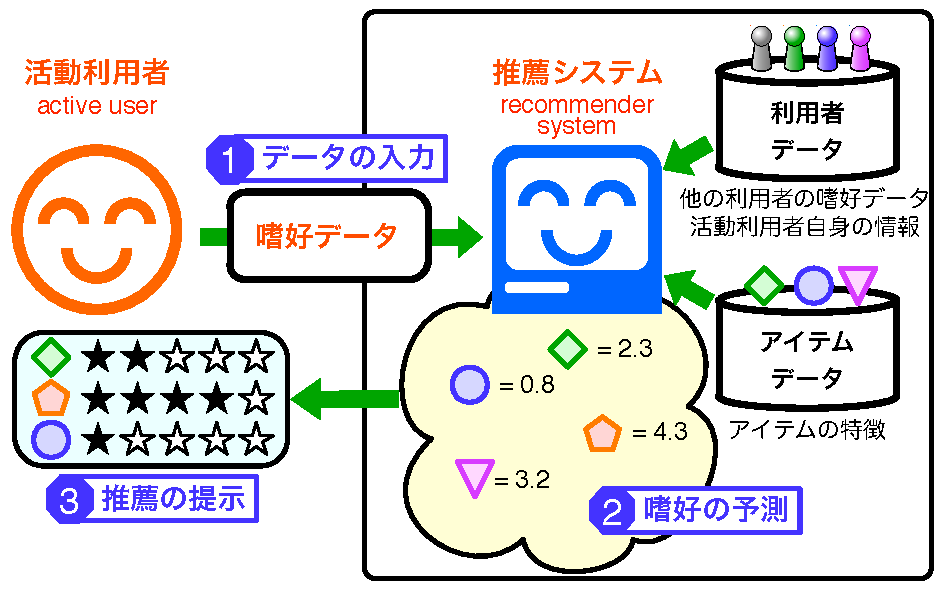
\includegraphics[width=0.8\fullwidth]{oipmodel.pdf}
\caption{推薦システムの実行過程(O-I-Pモデル)}
\label{fig:oipmodel}
\end{figure}

ここまでは,推薦システムを分類し,設計にあたって考慮すべき事項について述べてきた.ここでは,推薦システムがどのように実現されるかを見てゆこう.
推薦システムは,図\ref{fig:oipmodel}のように,データの入力,嗜好の予測,そして推薦の提示の三つの段階で推薦を行う.
これは\term{O-I-Pモデル}{output-input-process model}\cite{sigchi:03:01}とも呼ばれる.以下,これらの各段階の概要について述べる.

\begin{description}[style=nextline]
\item[データの入力]
推薦システムを利用して,推薦を受けようとしている人を\term{活動利用者}{active user}と呼ぶ.
活動利用者は自身の\termmain{嗜好データ}{preference data}を推薦システムに入力する.
嗜好データとは,いろいろなアイテムについての関心や好みの度合いを数値化したデータである.
この嗜好データの代わりに,関心のあるアイテムについてのより具体的な記述を検索質問や批評として,活動利用者に入力させるシステムもある.
また,推薦には,他の利用者の嗜好データ,アイテムの特徴データ,活動利用者自身の情報,推薦の状況や目的なども利用される場合があり,これらの情報を収集する場合もある.この段階については\ref{chap:input}章で述べる.
\item[嗜好の予測]
活動利用者の嗜好データに加え,収集しておいた利用者の他の情報やアイテムの情報を利用して,活動利用者がまだ知らないアイテムへの,活動利用者の嗜好を予測する.
嗜好の度合いを数値として予測する手法や,単に好きか嫌いかの識別をするだけの手法がある.
実現手段としては,機械学習の手法を用いるものや,人手によるルールを用いるものがある.
この段階については概要を\ref{chap:process}章で述べ,各種のアルゴリズムを第\ref{part:algorithm}部で紹介する.
\item[推薦の提示]
予測した嗜好に基づいて,目的に応じた適切な形式で,推薦結果を活動利用者に提示する.
%@@@ 評価の章を作ったら修正
このために,\ref{sec:systemtarget}節や\ref{sec:recomtask}節のいろいろな目的に応じた表示形式の変更や,\ref{sec:recomtype}節の各種指標のバランスを調整するためのアイテムの選別や順位付けの変更などを行う.
この段階については\ref{chap:output}章で述べる.
\end{description}

%!TEX root =  main.tex
%!TEX encoding = UTF-8 Unicode
\chapter{データの入力}
\label{chap:input}

ここでは,推薦システムの実行過程の最初の段階である「データの入力」について述べる.
この段階では,活動利用者に自身の嗜好データを,推薦システムへ入力させる.
嗜好データとは,利用者の各アイテムへの関心や好みの度合いをを数量化したものである.
システムによっては,この嗜好データの代わりに,活動利用者に検索質問や批評を入力させるものもある.
この検索質問は,アイテムの特徴についての制約条件を具体的に記述したものである.
例えば,レストランの推薦システムで,価格帯や,和洋中の別などを具体的に指示するために「価格は6000円以下で,和食の店」といった形式の検索質問を入力する.
こうした検索質問は,情報検索やデータベースのクエリ検索の技術がほぼ転用できるので,ここでは,嗜好データについて述べる.
さらに,これら嗜好データや検索質問で表された,活動利用者の嗜好パターンの以外のデータも推薦システムは利用する.
このようなデータとして,活動利用者以外の利用者の嗜好データ,アイテムの特徴,利用者の年齢や性別などの情報,現在位置などの利用状況を示す情報などがあり,これらにつても述べる.
なお,嗜好データの収集全般については,文献\cite{jjsai:04:05}にまとめられている.
また,文献\cite{sigir:01:01}は,推薦システムの利用者へのアンケート調査結果に基づいて,入力インタフェースについての設計指針を示している.
アイテムについての情報は,利用者が評価するときに見えるようにしておくと,システムへの満足が高まると報告している.

\section{暗黙的と明示的な嗜好データの獲得}
\label{sec:getprefimpexp}
\index{嗜好データ}\index{preference data}

\begin{table}
\centering
\caption{嗜好データ獲得法の長所と短所}
\label{tab:getprefcomp}
\begin{tabular}{l@{\qquad}c@{\,:\,}lc@{\,:\,}l}\toprule
 & \multicolumn{2}{c}{明示的} & \multicolumn{2}{c}{暗黙的} \\\midrule
データ量       & × & 少ない & ○ & 多い \\
データの正確さ & ○ & 正確 & × & 不正確 \\
未評価と不支持の区別 & ○ & 明確 & × & 不明確 \\
利用者の認知   & ○& 認知 & ×& 不認知\\
\bottomrule
\end{tabular}
\end{table}

まず,嗜好データを獲得するアプローチは,おおきく暗黙的と明示的の二種類に分けられる.
明示的な獲得とは,利用者に好き嫌いや,関心のあるなしを質問し,利用者に回答してもらう方法である.
もう一方の暗黙的な獲得とは,利用者の行動をから,利用者の嗜好や関心を推察することで嗜好データを得る方法である.
例えば,購入したり,閲覧したりしたアイテムには,利用者は関心があるとみなしたりする.

まず,二つの嗜好データの獲得法を比較する.
これらの獲得法の長所と短所を表\ref{tab:getprefcomp}にまとめた.
データ量については,利用者の嗜好の予測には統計的な方法が用いられるので,予測を正確にするにはより多くのデータを収集できた方が有利となる.
しかし,質問に答えるといった手間を利用者は嫌うことが多いため,明示的な獲得では多数のデータの収集は難しい.
よって,これらの点では暗黙的な手法が有利である.

データの正確さについては,暗黙的な獲得では,誤ってクリックしてしまったとか,人に頼まれて購入したなどの理由で,本当は関心がないものも,関心があるとみなされてしまう場合がある.このため,収集されたデータの正確さにおいては明示的な獲得が優れている.

利用者に明示的に評価してもらう場合では,アイテムを利用者が評価したかどうかはもちろん明確である.
しかし,暗黙的な評価では,利用者がそのアイテムに対して積極的な行動をしなかったことをもって,そのアイテムへの不支持とみなす場合がある.
例えば,閲覧しなかったアイテムは好きではないとみなしたとする.
このとき,アイテムについて未評価であることと不支持であることの区別ができない.
場合によっては,閲覧していないために,利用者が好むアイテムを嫌いだとシステムがみなすこともある.

最後の利用者の認知とは,利用者が自分の嗜好データをいつ,どのように取得されたかを知っているかどうかということである.
システムが提示した推薦は,利用者がその根拠を把握していた方が受け入れられやすい.
暗黙的な獲得では,嗜好データを意識的に入力していないので,推薦が根拠なくなされたもののように感じられやすく不利である.

\section{明示的な獲得}
\label{sec:explicitrating}
\index{明示的評価}\index{explicit rating}

アイテムを利用者に提示し,利用者にそのアイテムに対する好みの度合いを答えてもらう明示的な嗜好データの獲得について詳細を述べる.

\subsubsection{評価の動機付け}

明示的な獲得法では,利用者はアイテムを評価することを面倒だと思うので,暗黙的な方法に比べて多数の嗜好データを集めにくいと述べた.
\cite{sigir:01:01}では,利用者は推薦の精度が向上するなど,評価付けによるメリットが明確であれば,ある程度の手間をかけて評価付けをするとの調査結果を報告している.
よって,利用者に評価をさせるような動機付けは重要である.

自身への推薦の精度を向上させるということは,利用者にとって主な動機付けとなる.
だが,管理者が想定するようなこの動機以外にも,自分の意見の表明をするためや,他の利用者の手助けになるということを動機とする場合もある\cite{jacm:04:01}.
これらの動機は,利用者の評価数の順位の公開などによって喚起することができる.
さらに,明示的にインセンティブを与えることも考えられる.
文献\cite{ieeem:07:05}は,情報検索の結果の順位付けに,他の利用者の評価を利用する,一時的個人化の推薦システムを提案している.
このシステムでは,市場の考えが導入され,検索結果を閲覧するには,ポイントの支払いが必要である.
閲覧する文書の,被評価数が多く,評価が高いほど多くのポイントを支払う必要がある.
一方,ポイントは,検索した結果を評価することで獲得でき,被評価数が少なく,高い評価をすると獲得ポイント数は増える.
すると,検索をするために,検索結果の評価をする必要が生じるため,積極的な評価付けが期待できる.

\subsection{採点法と格付け法}

利用者が好みの度合いを答えるには,それを測る尺度が必要になる.
好みの度合いを表す尺度として,$0\sim5$ や$-3\sim+3$ のような数値尺度を使う\term{採点法}{scoring method} や,上・中・下 や 適合・不適合 などの順序付カテゴリ尺度を使う\term{格付け法}{rating method}\cite{j:0036}が良く利用されている.
こうした方法は人間の聴覚や味覚などを定量的に計測する官能検査(sensory test)の分野で研究されてきた\cite{jb:016:00}.
採点法や格付け法は,単純な入力フォームを用いて,比較的多数のアイテムに対する嗜好データを得られることが利点である.

これらの方法を使ううえでの注意点を幾つか述べておく.
%まず,尺度の段階の数は,利用者が真に要求している嗜好の段階数と等し
%いことが望ましい.
文献\cite{sigchi:03:02}では,利用者は評価尺度の目盛りが細かい方を好む傾向があること,さらに,細かい評価で予測精度が向上することはないが悪くもならないことを報告している.
よって,目盛りは細かめに設定することを推奨している.
さらに,${-}3$〜${+}3$の尺度で,中立の$0$を抜いた尺度を使うと,中立の評価の多くは弱い肯定的な評価$+1$に移されること,予測評価値を見せながら評価させると,利用者はそれに「引きずられた」評価をすることも報告している.
\ref{sec:recomtask}節で述べた適合アイテム発見を目的とする場合,目的に適合/不適合の2段階でも十分な場合が多いが,評価閲覧タスクでは,どれくらい不要なアイテムを除外したいかは利用者次第なので,より詳細な多段階の尺度を用いる方が良いだろう.
次に,質問の仕方にもいろいろな配慮をすべきである.
例えば,採点法では等間隔の尺度を連想させるように,等間隔の目盛りを見せるなどの工夫がある.これらの配慮については中森の\cite{jb:022:00}を参考にされたい.
%@@@ recsys:11:11:01

\subsection{評価値の揺らぎや偏り}

採点法や格付け法は大量の嗜好データを比較的に容易に得られるので多用されてきたが,当然ながら欠点もある.
先に,明示的な獲得は暗黙的な獲得と比べてより正確に利用者の嗜好を評価できると述べた.
だが,絶対的には不正確さや揺らぎがある.
真の嗜好の度合いは,脳の活動を直接観測するなどすれば将来的には計測できるであろうが,現在のところは厳密には計測できない.
そのため,揺らぎがあるかどうかの直接的な証明はできない.
よってここでは,採点法や格付け法によって計測した評価値が,真の評価値と乖離している間接的な証拠と,その乖離の原因を示す.

まず,評価値の揺らぎの証拠を示す.
官能検査の研究では,たとえ被験者が同じ評価値を与えていても,人によって嗜好の強さが違っていたりとか,時間がたつと一貫性が保たれなくなる問題があることが経験的に知られていた\cite{lncs:04:01}.
ソムリエなど訓練された被験者が,同一セッション内,すなわち,時間をあけずに連続して評価した場合でなければ,尺度を一定に保つことは難しいとされている.
嗜好データについても,一度映画を評価付けしたあと,6週間後にもう一度同じ被験者に同じ評価付けさせると,二つの評価値の間の相関は
0.83であったとの報告がある\cite{sigchi:95:01}.
文献\cite{sigchi:03:02}でも同様の報告がされている.
同一セッション内でも,寿司の嗜好について採点法で尋ねたのち,無関係な質問を幾つかしてから,下記の順位法で再び同じアイテムについて嗜好を質問すると,68.3\%の被験者の回答に不一致が観測された\cite{jpublist:043}.
これらの実験結果は,嗜好データには揺らぎがあることを示している.
他に,代表的な映画評価データにおいて,いろいろな工夫をしても,平均絶対誤差(MAE)を5段階尺度で0.73の「魔法の壁 (magic barrier)」より小さくできないことから,評価値そのものに揺らぎがあることが示唆されている\cite{jacm:04:01}.
以上のように,絶対的な評価値を使う採点法や格付け法では,被験者は,質問時期の違いなどにより揺らぎが生じるといえるだろう.

\begin{figure}
%(a) GroupLens   5.6  10.8  26.1  34.9  22.6
%(b) Amazon.com  7     5     8    20    60
%(c) 寿司        7.9   9.1  22.6  22.7  37.5
\centering
\subcaptionbox{MovieLens \cite{misc:129}\label{fig:prefdist:a}}%
{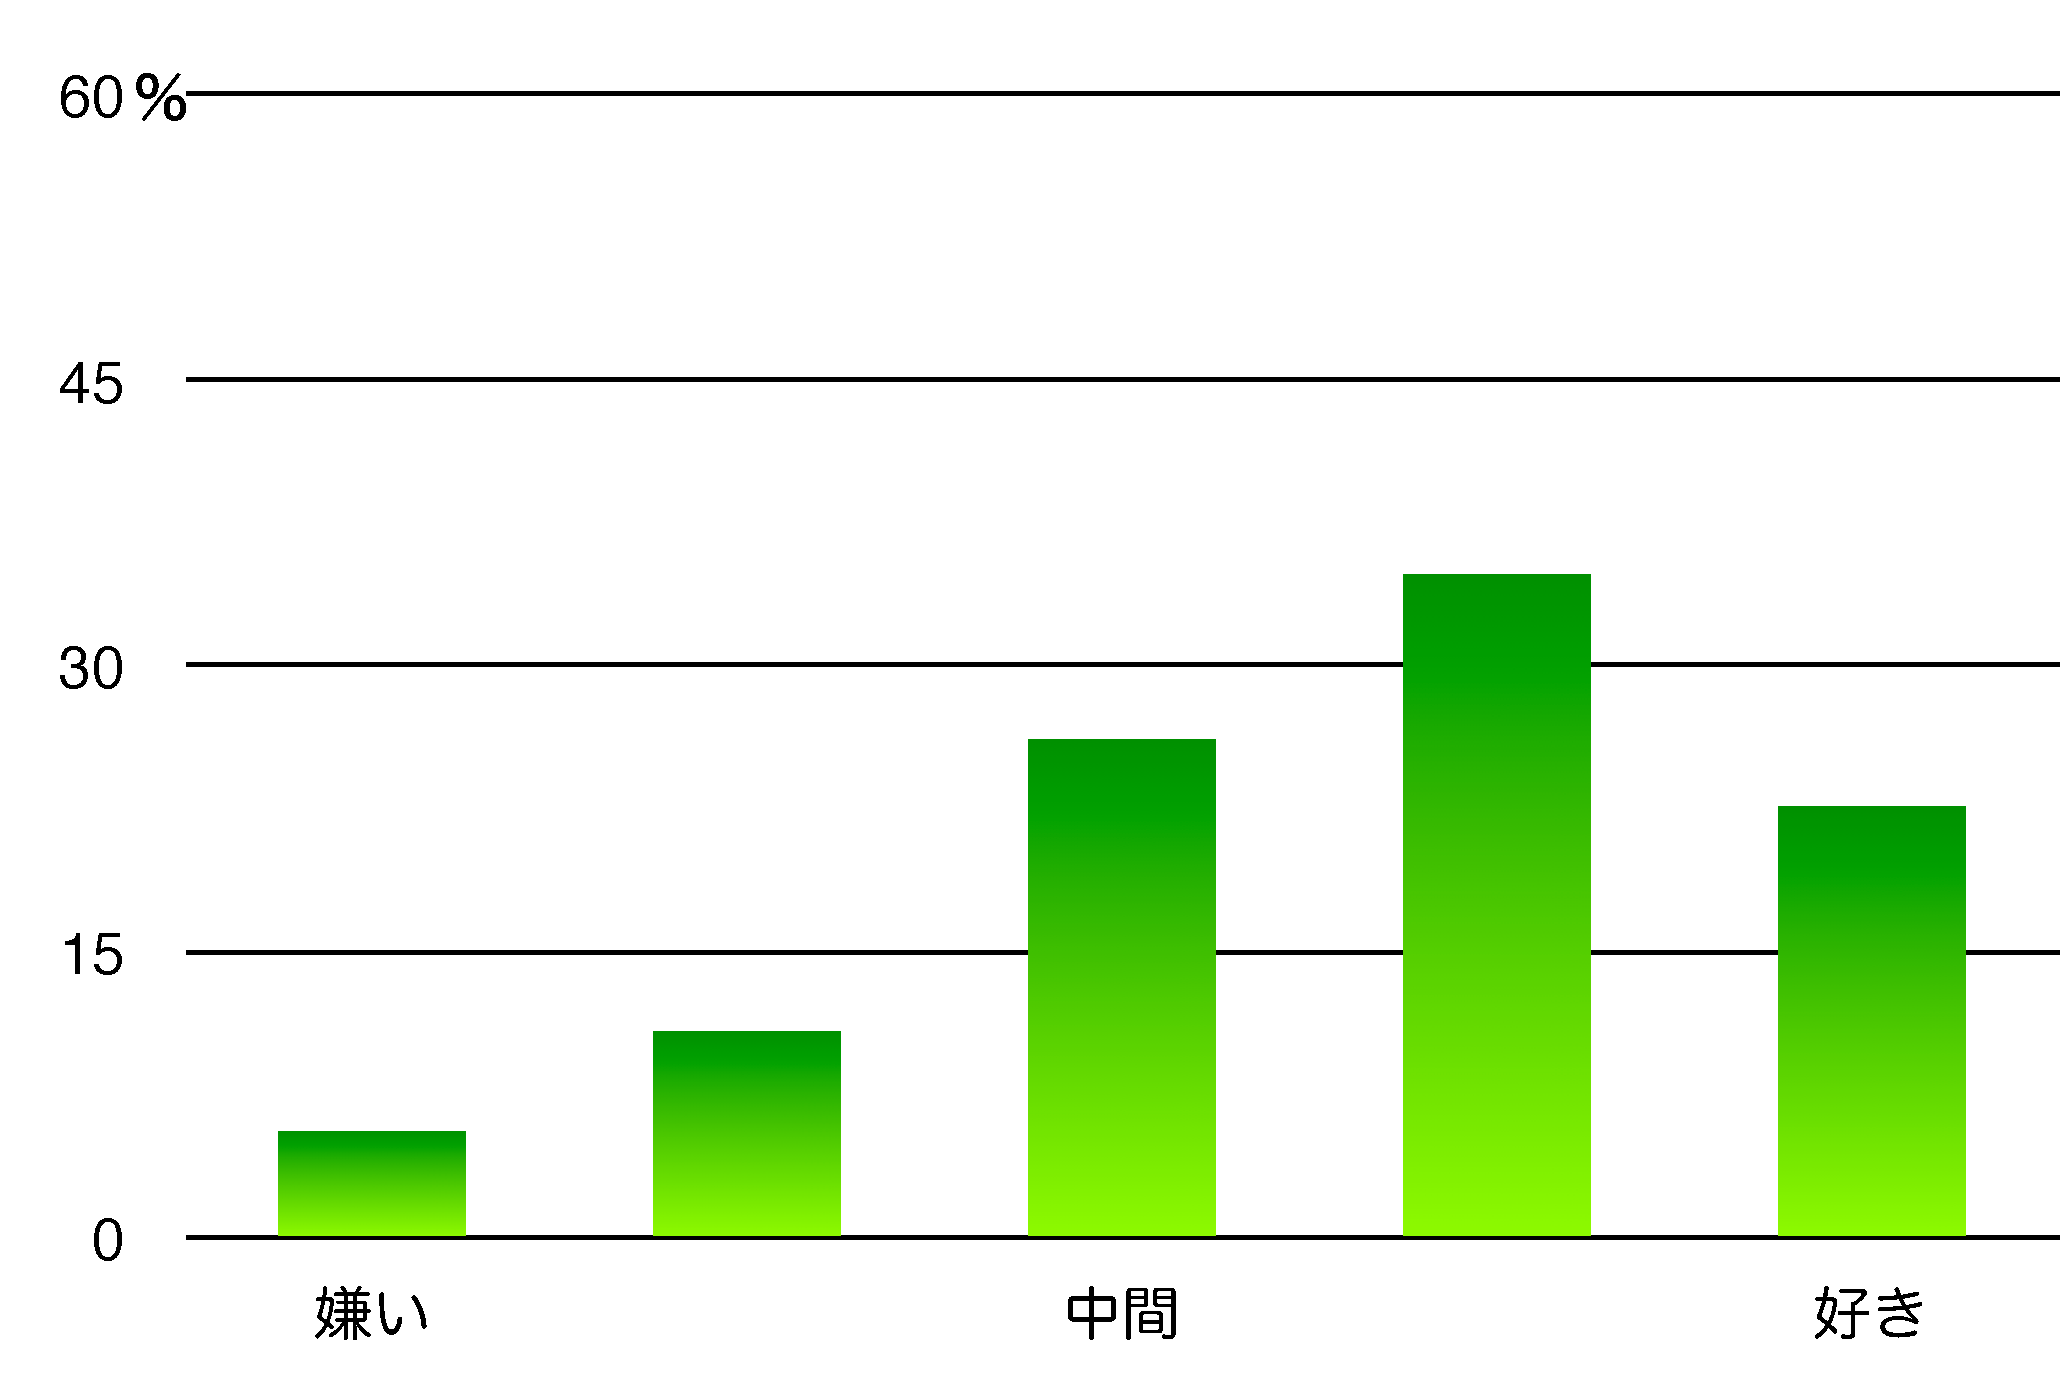
\includegraphics[width=0.6\linewidth]{rating-score1.pdf}}\\\medskip
\subcaptionbox{Amazon.com \cite{misc:007}\label{fig:prefdist:b}}%
{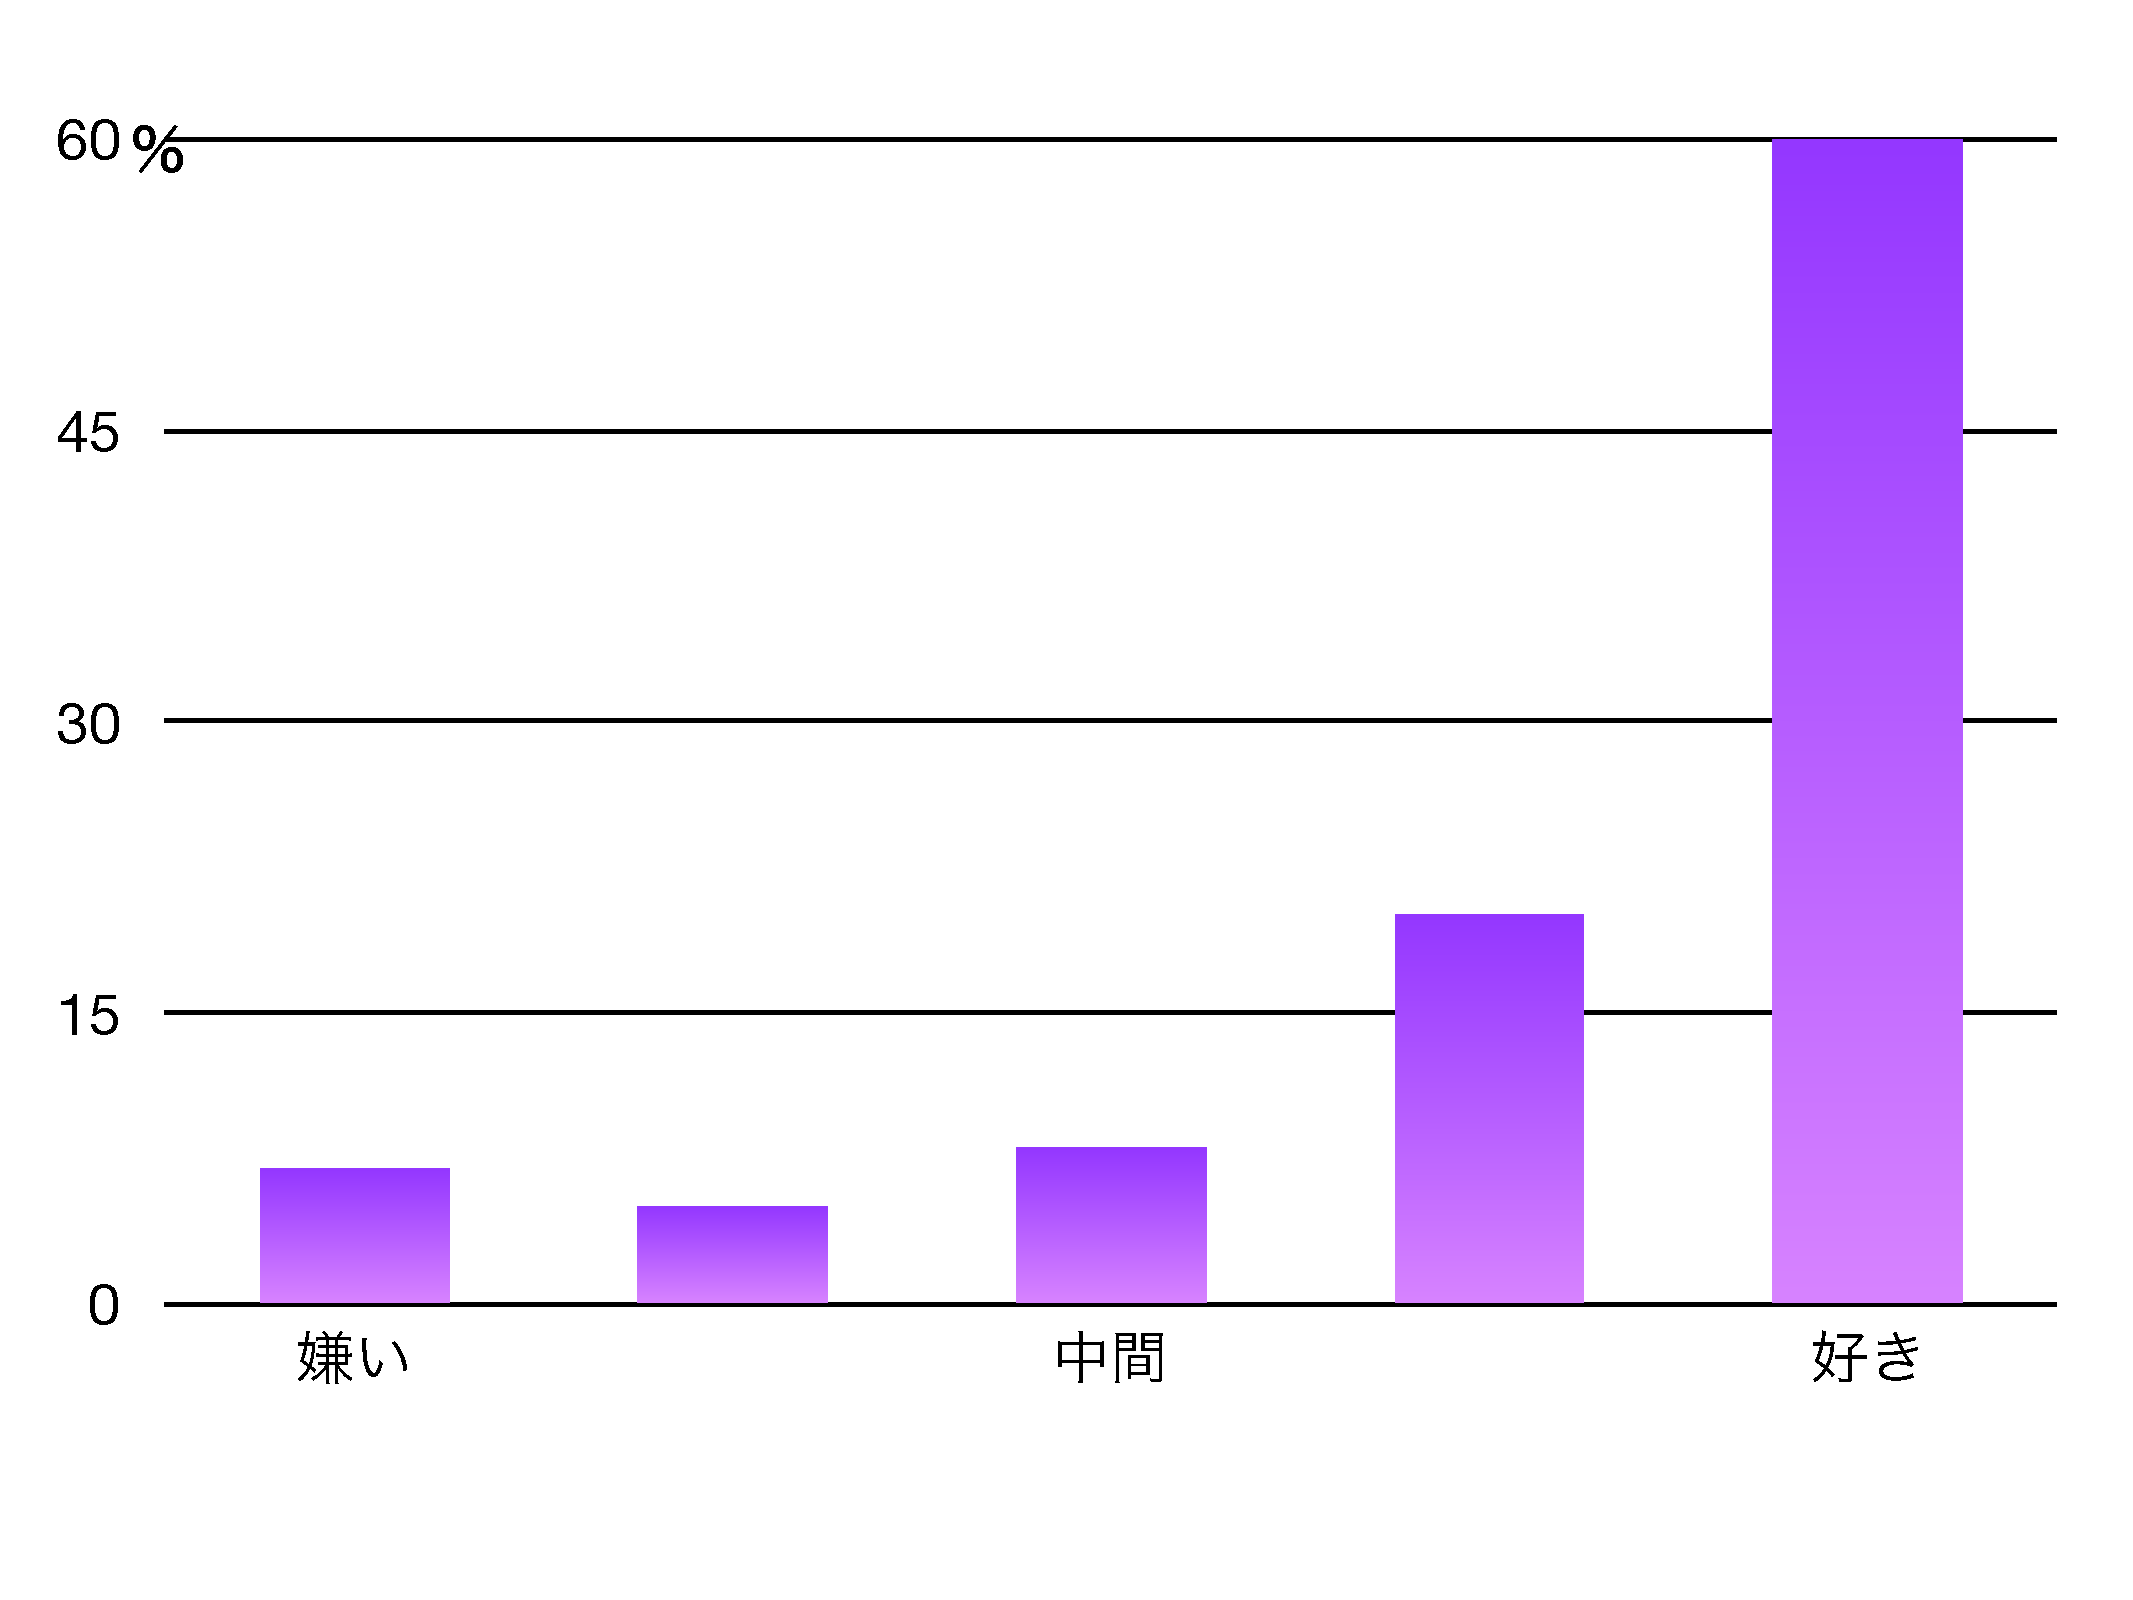
\includegraphics[width=0.6\linewidth]{rating-score2.pdf}}\\\medskip
\subcaptionbox{寿司 \cite{misc:140}\label{fig:prefdist:c}}%
{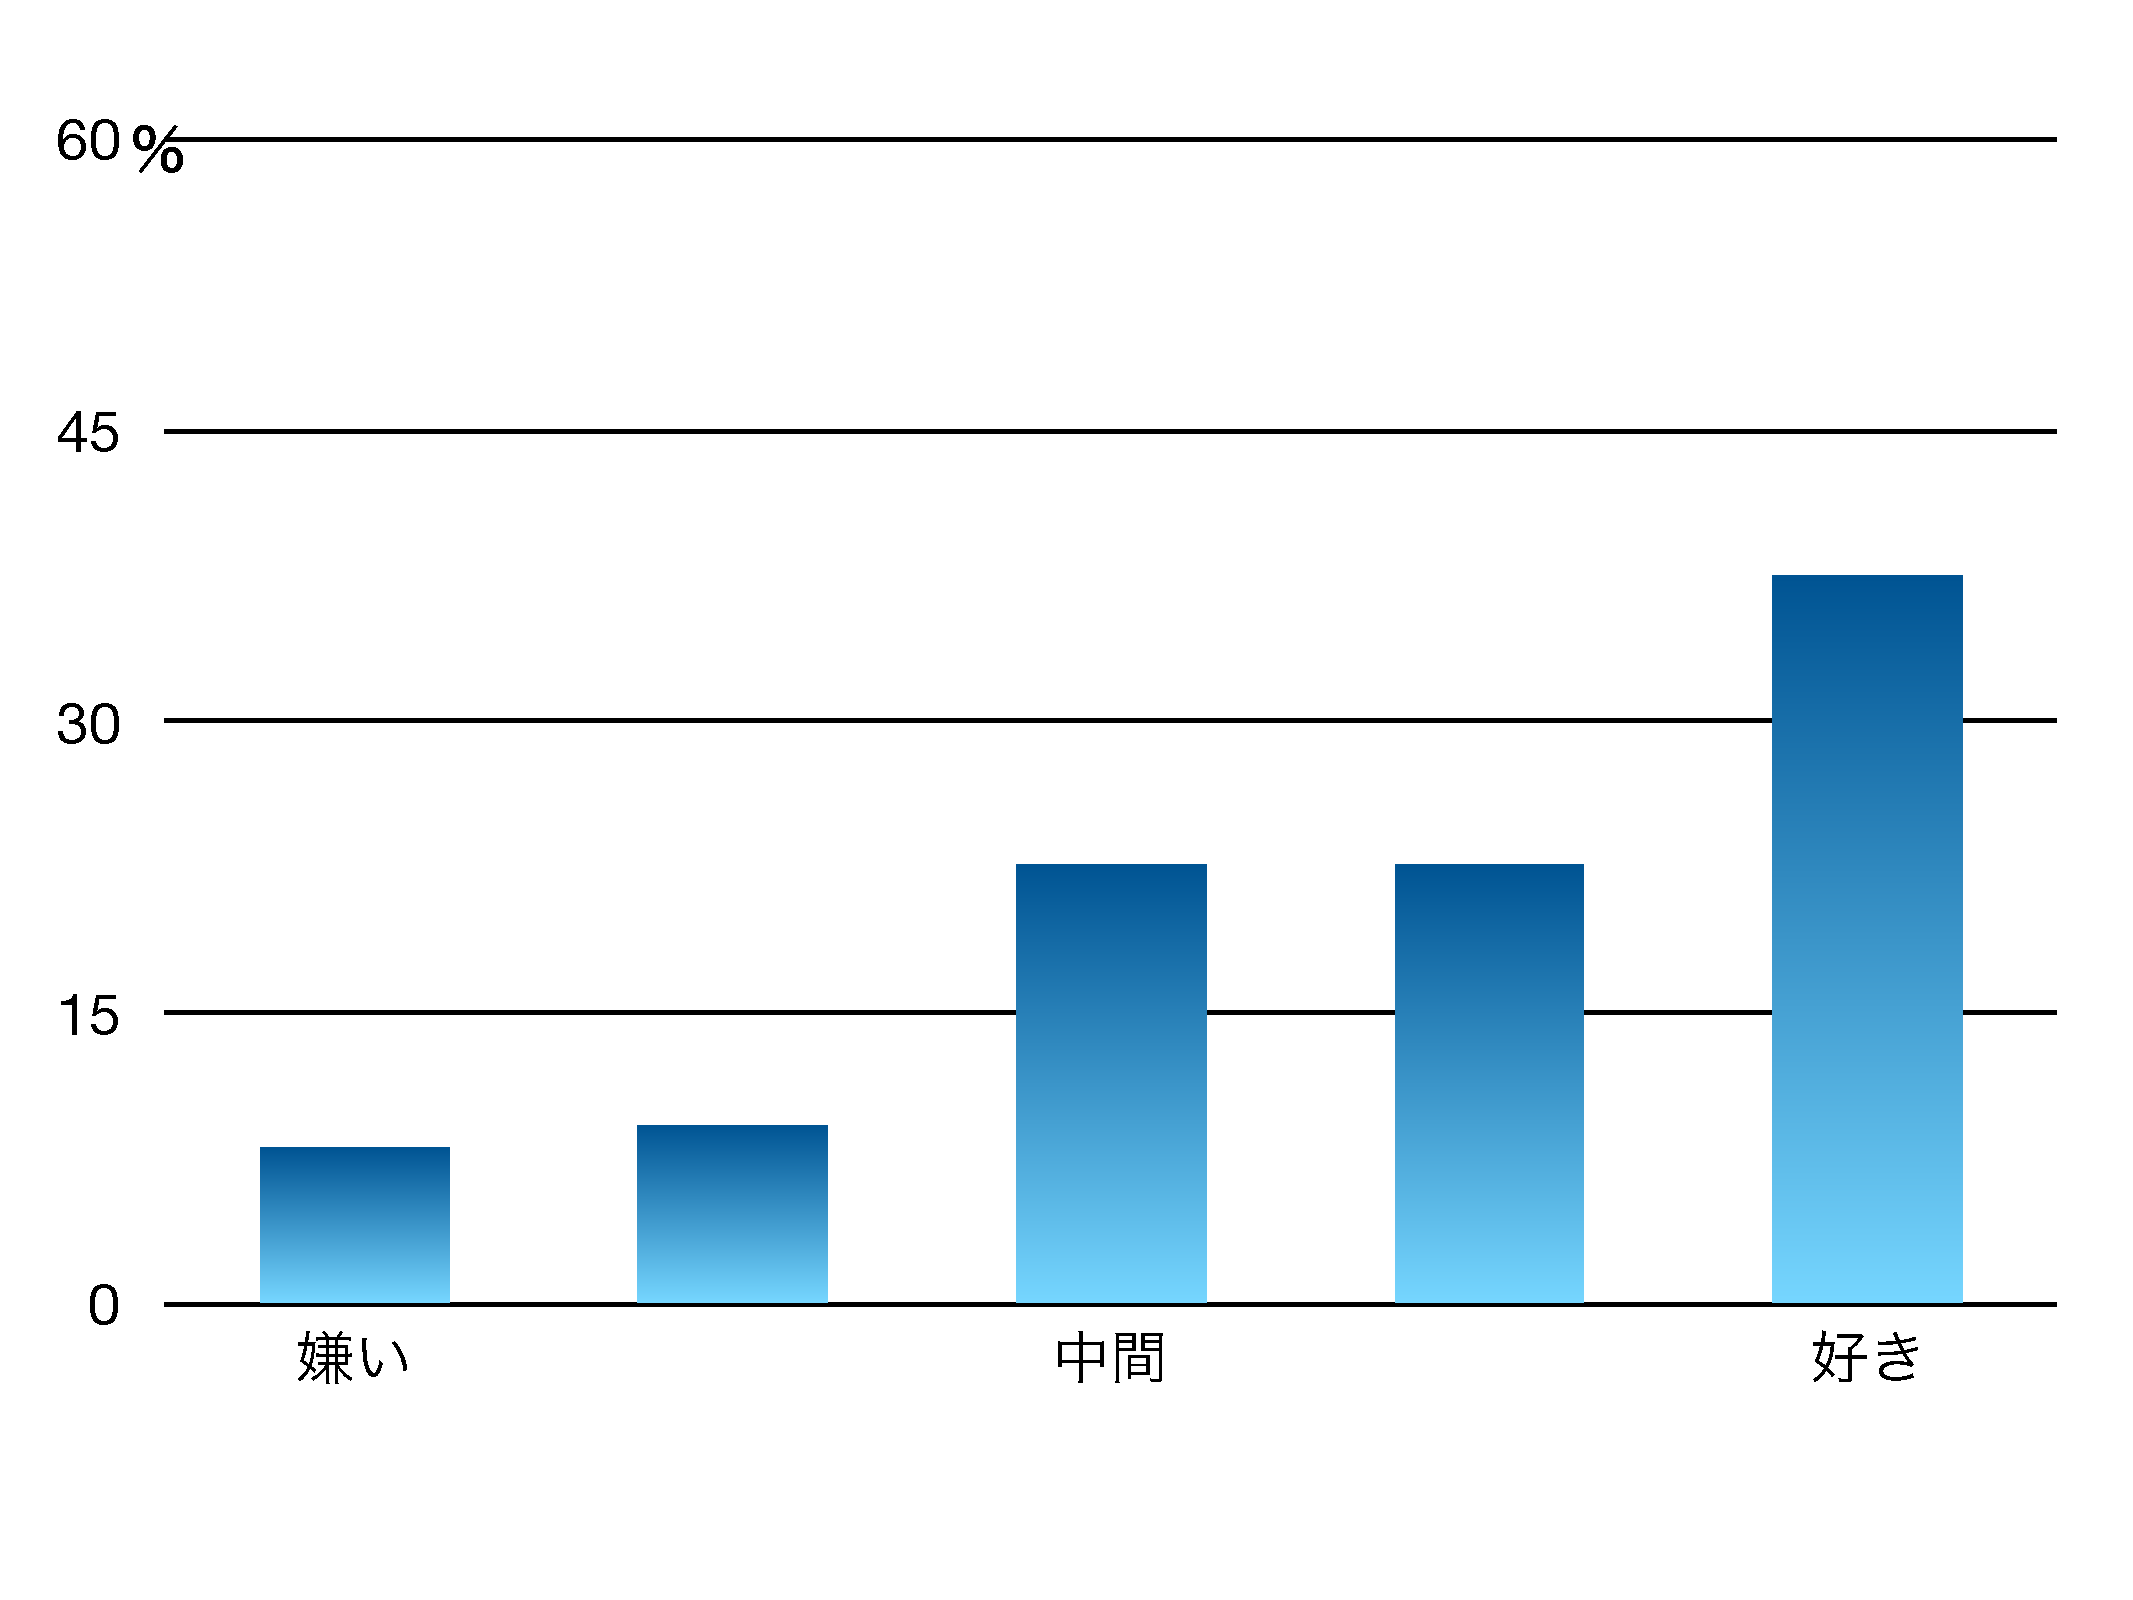
\includegraphics[width=0.6\linewidth]{rating-score3.pdf}}
\caption{アイテムへの評価値の分布}
\label{fig:prefdist}
\end{figure}

次に,評価値の偏りについて述べる.
図\ref{fig:prefdist}に,5段階の採点法を用いた3種類の嗜好データの,評価値の分布を示す.
それぞれ,\subref{fig:prefdist:a}~MovieLensの100万要素のデータ集合\cite{misc:129},\subref{fig:prefdist:b}~電子商取引サイトAmazon.com\cite{misc:007},\subref{fig:prefdist:c}~寿司の嗜好調査\cite{misc:140,epublist:064}での分布である.
どのデータでも,『好き』の方へ明らかに偏っている.
この偏りの原因には,サンプリングと真の嗜好からの乖離の二つが考えられる.
サンプリングの偏りの原因として,図\ref{fig:prefdist:a}や\subref{fig:prefdist:b}では,利用者が,関心がある選択的にアイテムを評価していることや,図\ref{fig:prefdist:b}や\subref{fig:prefdist:c}では,市場の淘汰を受けて人気のあるアイテムのみが評価候補となっていることが挙げられる.
このようなサンプリングの偏りは,\ref{sec:prederr}節で指摘したように,予測誤差の正確な評価を妨げる.
真の嗜好から乖離する理由としては,利用者個人がもつ心理効果の影響が考えられる.
例えば,過剰な酷評は社会的通念的に良くないとの考えをもつ人には,全体的に評価が高くする寛大効果 (leniency effect)が見られ,あいまいな判断や質問では中心のスコアを選びやすい中心化傾向 (central tendency)などが生じる\cite{jb:026:00}.
さらに,質問の仕方による影響も考えられる.
例えば,尺度の一方だけが連続して選ばれるように質問を配列すると偏りが生じる場合がある\cite{jb:022:00}.
%例えば,5を選び続けると,本当は4でも5と答えてしまったりする.
しかし,推薦システムでは,推薦結果の提示と嗜好データの収集を兼ねるため,利用者が好むと予測される順にアイテムを並べ評価付けさせることがよく行われる.
すると,高い評価値が高頻度で連続してしまう.
このように,設計上の制限により,偏りを生じるような質問の仕方をしてしまうという問題もある.

\subsection{順序の利用}

そこで,採点法や格付け法以外の調査方法の利用が考えられる.
文献\cite{sigir:99:02}では,利用者の類似度評価においてスコアの順位関係だけを考慮することや,利用者ごとの平均評価値を0に正規化することで予測精度が向上することを報告している.
このことは,採点法で得た評価値の絶対的な値ではなく,相対的な大小が重要であることを示唆しているといえるだろう.
また,採点法や格付け法で得られる量は,本質的には大小関係にのみ意味がある順序尺度\cite{eb:036:00,jj:015}であると指摘されている
\cite{jb:022:00}.
そこで,好きなものから嫌いなものへ順に,複数の対象を並べるという\term{順位法}{ranking method}を利用する「なんとなく協調フィルタリング」
\cite{epublist:039,epublist:064}を神嶌は提案した.
少なくとも調査したデータにおいて,順位法の採用で予測精度が向上した.
ただし,順位法にも問題点がある.
同時に多数のアイテムを整列するのは難しいので,大量の嗜好データをまとめて得ることは難しい.また,評価は常に相対的で,絶対的な評価は得られない.そのため,相対的に良いものを選ぶような意志決定には役立つが,絶対的な評価が求められる評価閲覧タスクなどには向かない.

官能検査の調査方法としては,取り出したアイテム対のどちらが良いかを指定する一対比較法(paired comparison)や,幾つかの候補の中から最良のものを指定させる択一法 (choice method) などもある.
これらの方法についての研究は著者はまだ知らず,今後の研究が待たれる.

\section{暗黙的な獲得}
\label{sec:implicitrating}
\index{暗黙的評価}\index{implicit rating}

暗黙的な嗜好データの獲得では,アイテムに関連した,利用者の行動に基づいて,そのアイテムについての嗜好を判断する.
利用者があるアイテムを閲覧したり,購入したりすると,これらの行動はそのアイテムへの潜在的な肯定を示していると考えられる.
また,購入は閲覧よりもより強い肯定を示すとも考えられる.
このような行動による潜在的な嗜好の強弱をNicholsは論じている\cite{misc:088,ej:048}.
強い嗜好を表すものから順に次のような行動を挙げている.
\begin{center}
\small
\begin{tabular}{llll}
1. Purchase & 2. Assess & 3. Repeated Use & 4. Save/Print \\
5. Delete & 6. Refer & 7. Reply & 8. Mark \\
9. Terminate Search & 10. Examine/Read & 11. Consider & 12. Glimpse \\
13. Associate & 14. Query & &
\end{tabular}
\end{center}
文献\cite{ieeem:07:01}では,閲覧,ビデオのプレビュー,購入の3種類の
行動それぞれを暗黙的な肯定入力と考え,それぞれの行動別に利用者間の
類似性を計算している.

他の暗黙的な獲得法として次のようなものがある.
推薦リストの上位からA, B, C,…とアイテムを閲覧してCを選んだとき,AやBを見たにも関わらずCを選択したことから,AよりC,BよりCを好むという相対的嗜好順序を得る方法\cite{kdd:02:01}が提案されている.
閲覧するという行為だけでなく,その時間を計測することで,より詳細な情報を得る方法などもある.
また,新たに入力装置を導入して,利用者の行動情報を収集し,そこから暗黙的に嗜好データを獲得する試みもある.例えば,マイクで収集した発話内容\cite{trjsai:07:01}や,アイカメラを使って求めた注視領域\cite{trjsai:07:02}などを利用する試みなどである.

\section{嗜好データのその他の要因}
\label{sec:getprefother}

嗜好データで推薦に影響するその他の要因を挙げておく.
利用者が初めてシステムを利用するときに,特定のアイテム群について明示的に質問して,嗜好データを集めることが考えられる.
全ての利用者が共通に評価しているアイテム群があると,\ref{chap:cf}章の協調フィルタリングでは利用者間の嗜好の類似性を評価しやすくなる利点がある.
しかし,音楽のようにその場で少し聞かせて評価できるようなものならよいが,映画などは見たことがないものは評価しにくい.
よって,こうした共通アイテム集合を利用できるかどうかは推薦するアイテムの種類に依存する.

評価したときの時間情報も利用できる.
服飾品のように流行の影響がある場合には,時間がたった嗜好データはあまり有効ではないだろう.
また時間の前後関係に依存する\ref{sec:timeseries}節のような嗜好の予測方法もある.
単純な好き・嫌いではなく,Zagatのレストランガイドのように,味・サービス・内装といった項目ごとに分けて嗜好データを収集することもできる.
こうしたシステムとしては\cite{ieeem:07:02}がある.

\section{嗜好データ以外のデータ}
\label{sec:featuredata}

嗜好データ以外の,推薦に利用されるデータについてまとめておく.

\subsection{アイテムの特徴}

アイテムを特徴ベクトルで記述したデータで,内容ベースフィルタリングでは必須である.
推薦対象がテキストである場合はBag-of-wordsモデルでtf-idf重み\cite{j:0021}が一般に使われる.この場合多数の特徴量が得られるが,個々の特徴の推薦への寄与は小さい.
一方,推薦システムの設計者が意図的に選択した特徴は,多数は得られないが,個々の特徴はより推薦に寄与する.
こうした特徴には,映画の場合では監督や制作年,ラーメンであればスープや麺の太さといったものが挙げられる.
このように,明確な特徴の他に,アンケート調査などで獲得した印象などを特徴にする場合もある.映画の例では「悲しい」や「楽しい」といった印象語への採点法による評価の平均評価値などを特徴量として利用できる.

\subsection{個人属性の特徴}

利用者の年齢や性別などの\term{個人属性情報}{demographic information}も利用できる\cite{ej:050}.
これらの情報は嗜好と関連があると考えられ,マーケティングにおいてもデータベースマーケティングとして利用されてきた\cite{dmkd:01:01}.
%活動利用者以外の嗜好データも利用するシステムでは,その利用者の推薦
%における重要度\cite{tjsai:04:09}なども利用できる.
個人属性の特徴があれば,新規利用者に対しても推薦が可能になる利点があるが,プライバシー問題の観点から,その収集が困難である問題がある.
この問題に対しては,データの利用目的を説明すること\cite{sigir:01:01}や,\ref{chap:privacy}章のプライバシー協調フィルタリングの導入といった対処がある.

\subsection{利用状況の特徴}

推薦システムを利用する状況の情報である.
レストランを利用する場合などでは人数や場所の情報は推薦の制約になる\cite{tjsai:06:01,trjsai:06:01}.
また,システム側のコンテキストとして,商品の在庫や納期の情報など,推薦時には考慮すべき情報である.

%!TEX root =  main.tex
%!TEX encoding = UTF-8 Unicode
\chapter{嗜好の予測}
\label{chap:process}

嗜好の予測とは,活動利用者の嗜好データや,アイテムの特徴を用いて,活動利用者の各アイテムへの関心や好みの度合いを予測することである.

嗜好の予測段階の実現方法は大きく二つに分類される.
レンタルビデオ店で,顧客が見たい映画を推薦する場合を考えてみよう.
一つは,ファンである監督,好みのジャンルを利用者に尋ねてその条件に合ったものを選ぶ方法である.
これを,検索対象の内容を考慮して推薦をするので\term{内容ベースフィルタリング}{content-based filtering}と呼ぶ.
もう一つは,映画の趣味が似ている知り合いに,面白かった映画を教えてもらう「口コミ」の過程を自動化する方法である.
他の人との協調的な作業によって推薦対象を決めるため,この推薦手法は\term{協調フィルタリング}{collaborative filtering}や社会的フィルタリング (social filtering)と呼ばれている.

\begin{figure}
%(a) GroupLens   5.6  10.8  26.1  34.9  22.6
%(b) Amazon.com  7     5     8    20    60
%(c) 寿司        7.9   9.1  22.6  22.7  37.5
\centering
\subcaptionbox{内容ベースフィルタリング(間接指定型)\label{fig:cfcbf:a}}%
{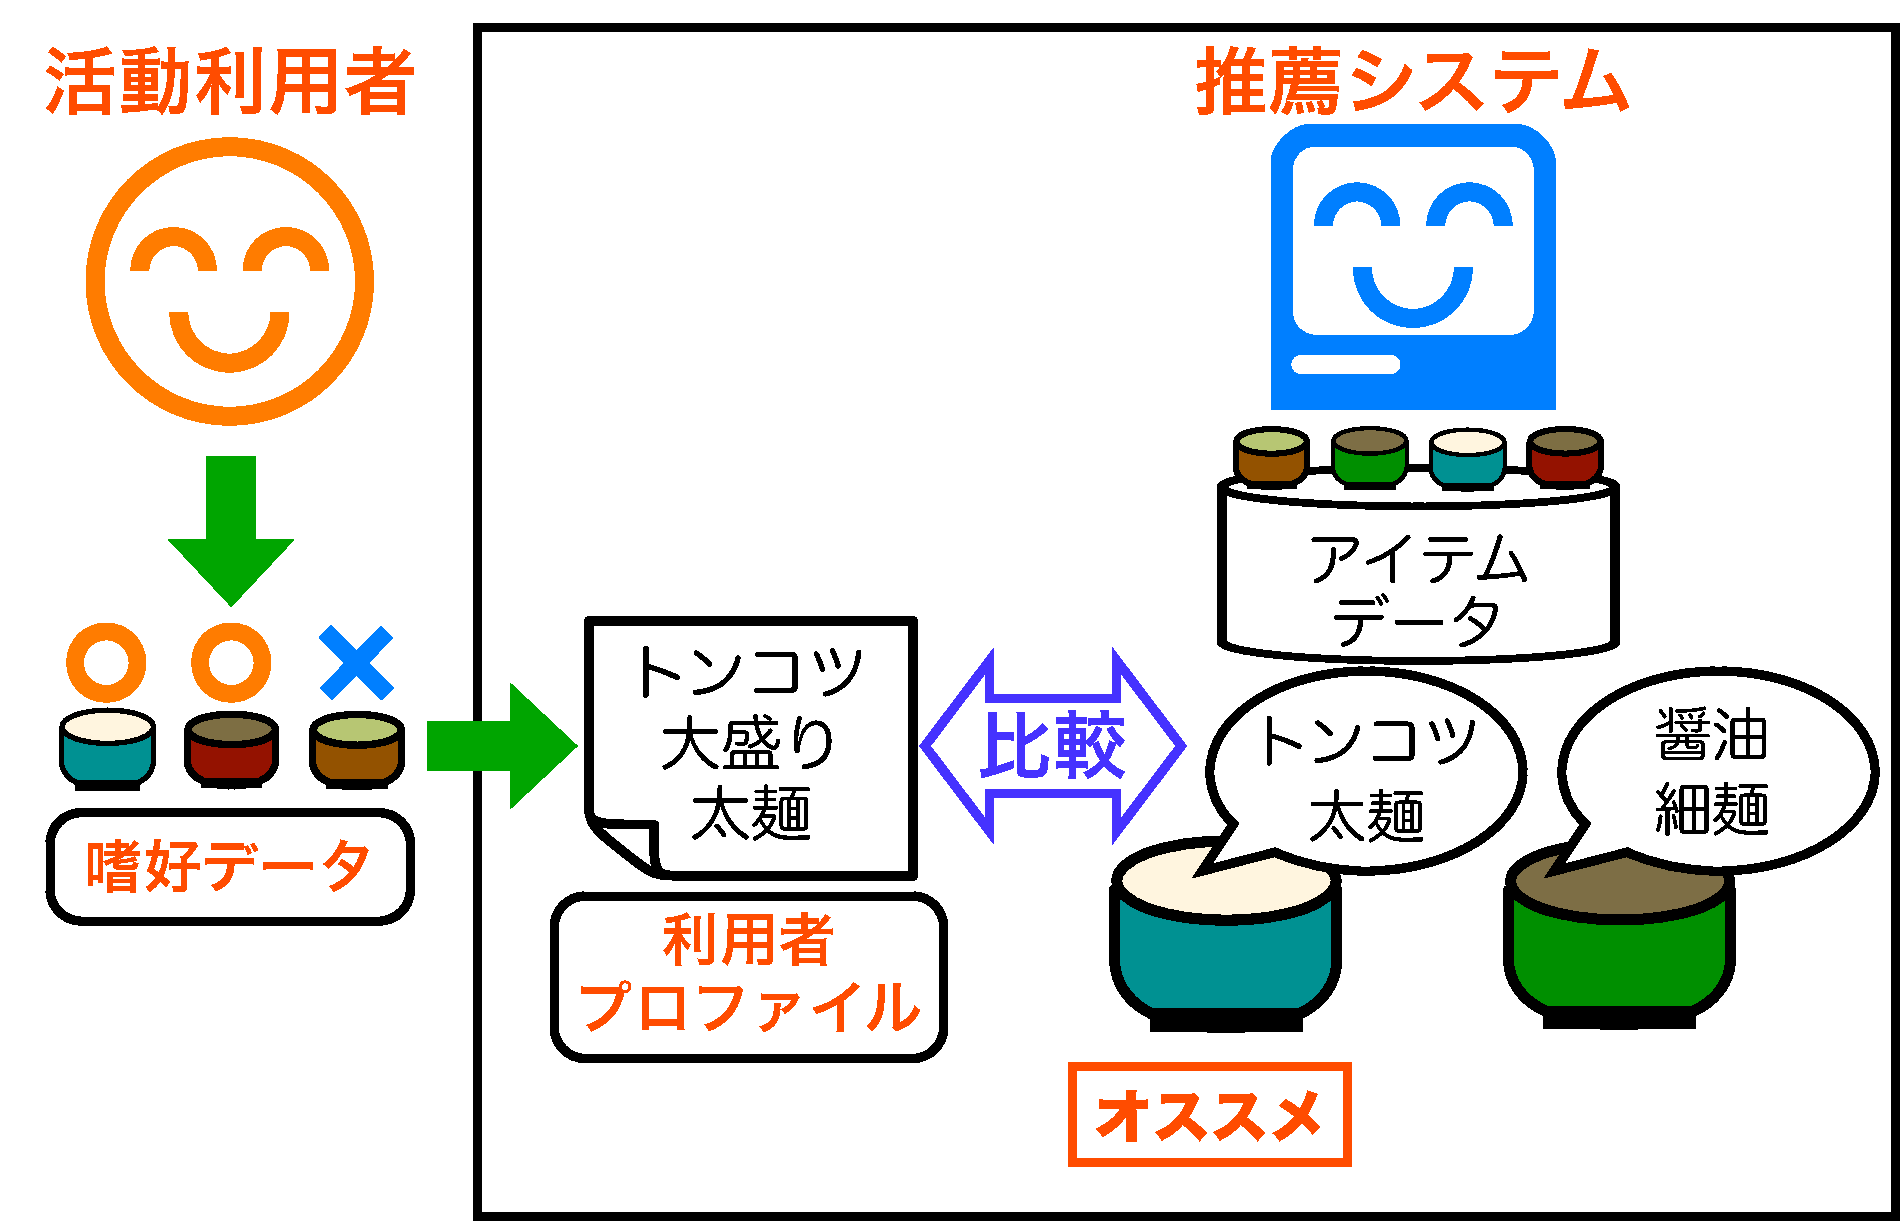
\includegraphics[width=0.6\linewidth]{rsyscategory-icbf.pdf}}\\\medskip
\subcaptionbox{内容ベースフィルタリング(直接指定型)\label{fig:cfcbf:b}}%
{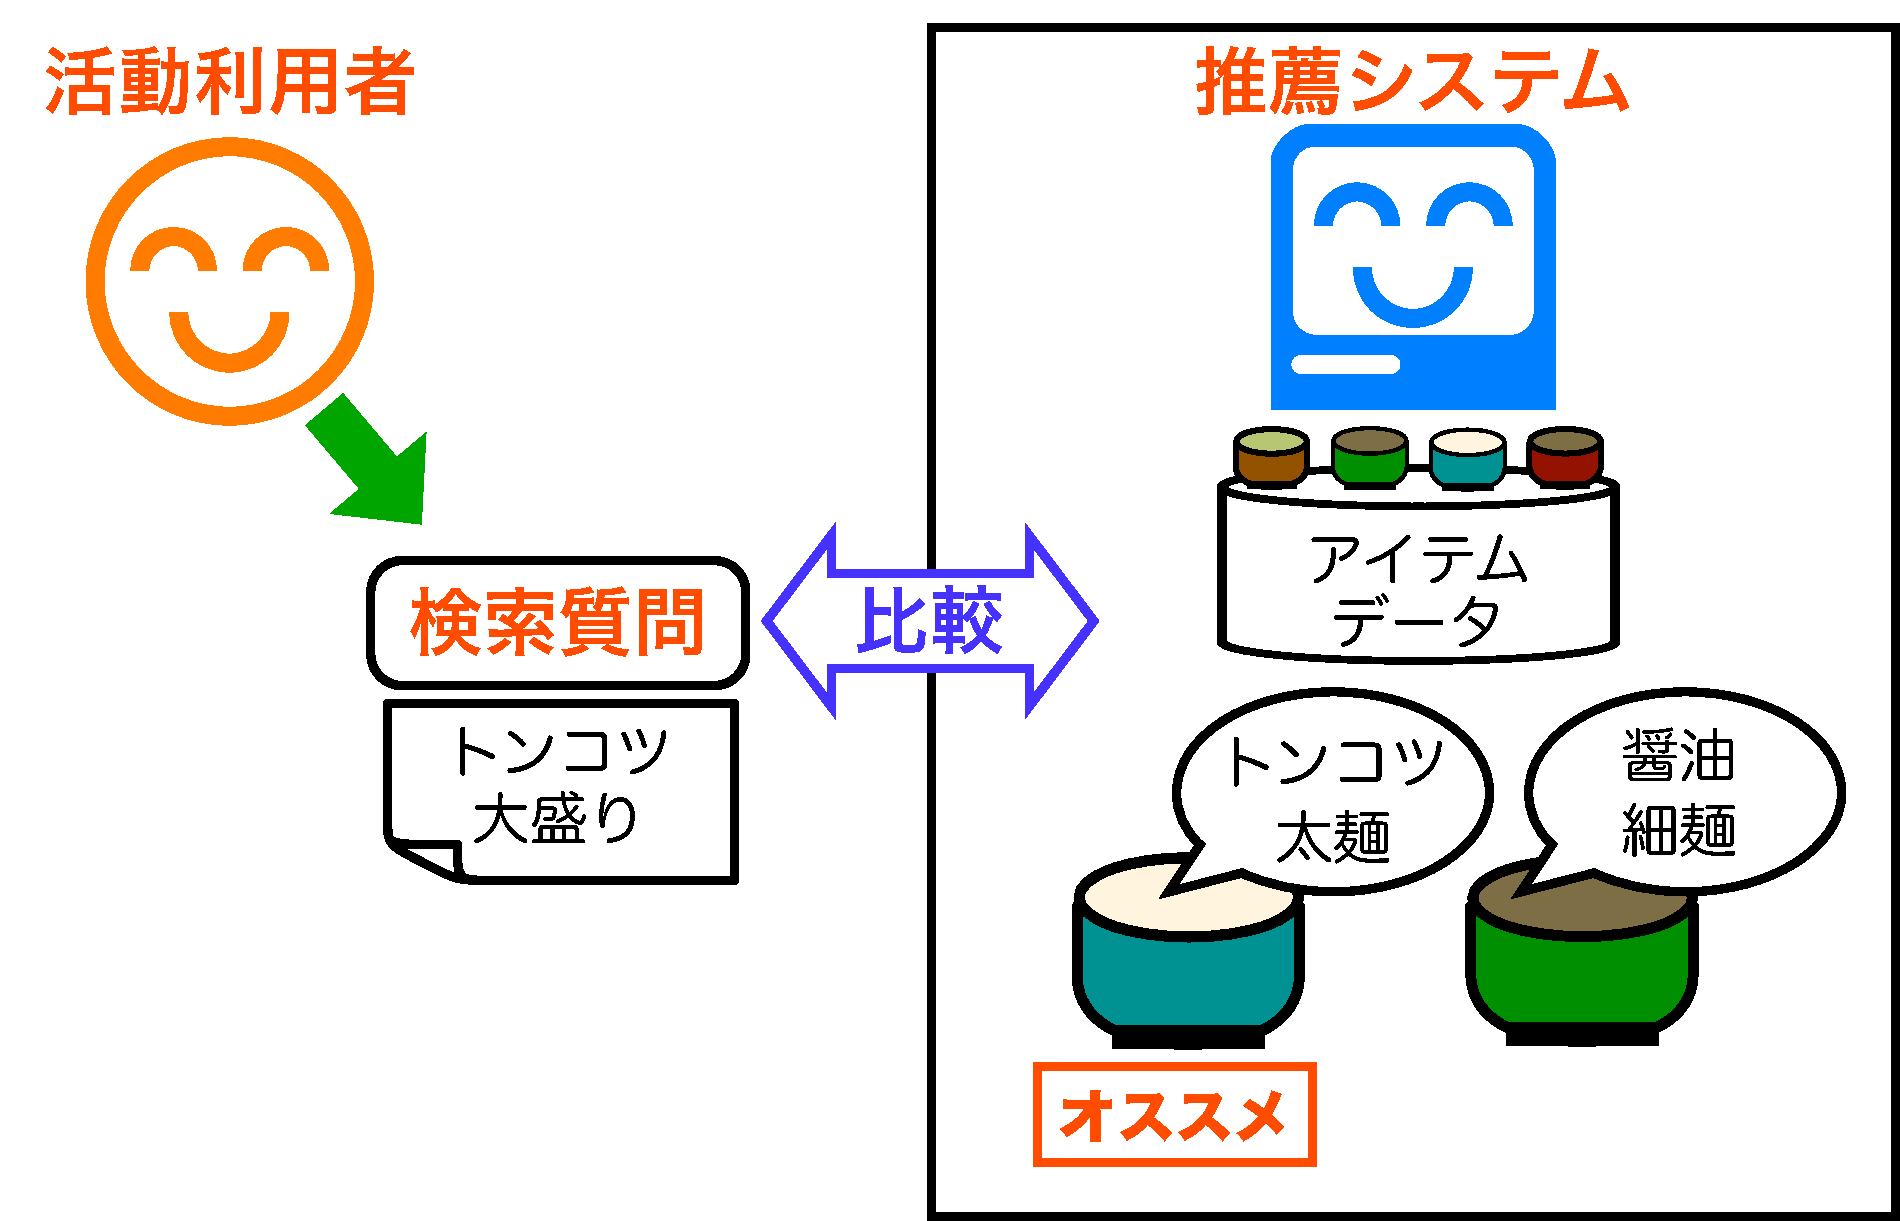
\includegraphics[width=0.6\linewidth]{rsyscategory-dcbf.pdf}}\\\medskip
\subcaptionbox{協調フィルタリング\label{fig:cfcbf:c}}%
{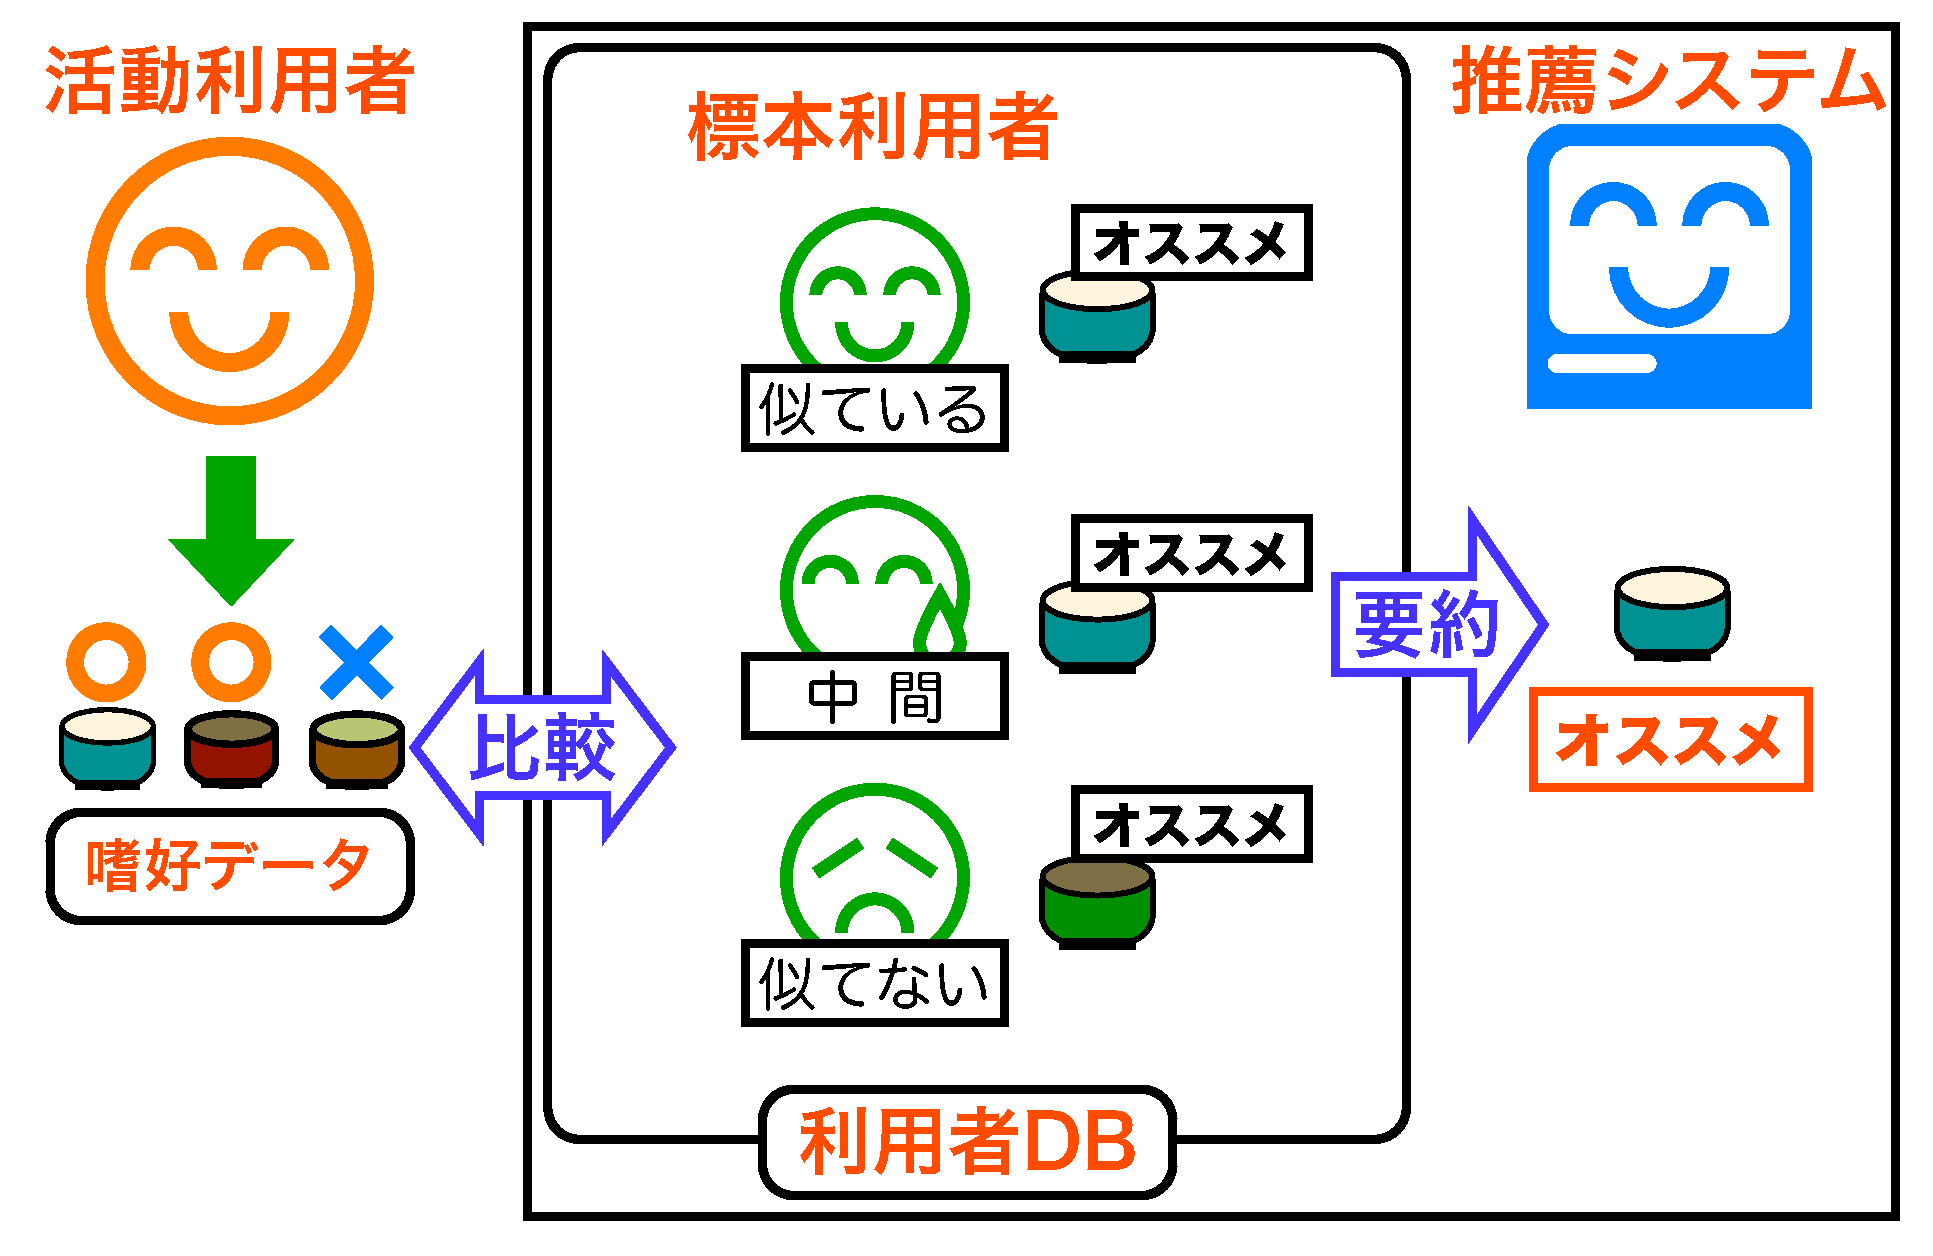
\includegraphics[width=0.6\linewidth]{rsyscategory-cf.pdf}}
\caption{内容ベースフィルタリングと協調フィルタリング}
\label{fig:cfcbf}
\end{figure}

現在では,どちらの方法にもいろいろな派生型が提案されているが,純粋な形では図\ref{fig:cfcbf}のように予測する.
内容ベースフィルタリング(図\ref{fig:cfcbf:a}と\ref{fig:cfcbf:b})では,アイテムの性質と利用者の嗜好パターンを比較して,利用者が好むと判断したものを推薦する.
このアイテムの性質は特徴ベクトルによって記述される.
特徴ベクトルとは,アイテムのいろいろ側面の性質を表す特徴を集めて,ベクトルの形にしたものである.
各特徴は,事前に定めた定義域中の値をとることで,そのアイテムの性質を表現する.
ラーメンの例を示そう.このとき,スープの種類,麺の太さ,価格といった特徴からなるベクトルでラーメンを表現する.
スープの種類という特徴は,トンコツ,醤油,塩のような定義域の値の一つをとり,価格という特徴では自然数がその定義域となる.
そして,ある特定のラーメン『トンちゃん』があるとすると
\begin{center}
\footnotesize
(スープの種類=トンコツ, 麺の太さ=細麺 ,…, 価格=650円)
\end{center}
といったベクトルで表現される.
こうした情報をいろいろなアイテムについて収集したものをアイテムデータと呼んでおく.
一方,利用者の嗜好パターンは\term{利用者プロファイル}{user profile}によって表す.
この利用者プロファイルを間接指定するシステムと,直接指定するものがある.
間接指定型(図\ref{fig:cfcbf:a})では,利用者のいろいろなアイテムに対する嗜好データ,すなわち,好き嫌いの度合いを定量化したデータを集める.
この嗜好データと,アイテムデータに基づいて,その利用者が好むアイテムの特徴のパターンを機械学習の手法でモデル化し,利用者プロファイルとする.
直接指定型(図\ref{fig:cfcbf:b})では,利用者が明示的に,自身が好むアイテムの特徴を表した検索質問(query)(批評(critique)ともいう)を入力する.
一般的な検索質問は「スープの種類は醤油で,価格は500円以下」といった,特徴に対する制約の形式だが,自然言語文などを扱えるものもある.
この検索質問はそのまま利用者プロファイルとして用いられる.
内容ベースフィルタリングでは,アイテムデータ中のアイテムの特徴ベクトルと,利用者プロファイルとを比較し,プロファイルに最も近い特徴ベクトルをもつアイテムを利用者が好むものと判断して推薦をする.

もう一つの協調フィルタリング(図\ref{fig:cfcbf:c})では,アイテムの性質は全く考慮しない.
その代わりに,システムが利用される前に,多くの利用者の,いろいろなアイテム対する嗜好データをデータベースに集積している.
このデータベースを\term{利用者データベース}{user database}(「利用者DB」と略す)と呼び,この利用者DBに嗜好データを登録している利用者を\term{標本利用者}{sample user}と呼ぶ.
さらに,今までの嗜好パターン,すなわち,どのアイテムを好み,どのアイテムを嫌うのかという傾向が類似している利用者は,これからも同じアイテムを好み,同じアイテムを嫌うであろうという仮定を導入する.
この仮定の下,活動利用者と,嗜好パターンが類似している標本利用者を見つけ,これらの標本利用者が好むものを活動利用者に推薦する.

なお,内容ベースフィルタリングは,いろいろな拡張が行われているので,厳密に定義するのは難しい.
文献\cite{ej:048}では,個人属性の特徴(\ref{sec:featuredata}節)などを用いず,アイテムの特徴のみを用いた,間接指定型の手法のみを内容ベースフィルタリングと定義している.
そして,上記の直接指定型にあたる知識ベース型や,デモグラフィックな特徴を使うものも,別の種類として細かく分類している.
しかし,細分化しても多種多様な手法を厳密に分類するのは実際には難しいので,本稿では,広義にとらえて,アイテムやデモグラフィックな特徴を利用するような方法は全て内容ベースフィルタリングとして扱う.
一方,これらの特徴を用いず,標本利用者の嗜好データのみを用いる方法を協調フィルタリングとしておく.

第\ref{part:algorithm}部では,協調フィルタリングと内容ベースフィルタリングの各種手法を順に紹介する.
さらにその後に,これら二つの手法を組み合わせるハイブリッド法について述べたのち,アルゴリズムの選択の指針について述べる.
これらの話題に移る前に,協調フィルタリングと内容ベースフィルタリングの長所と短所をまとめておく.

\section{内容ベースと協調フィルタリングの比較}
\label{sec:cfcbfcomp}

\begin{table}
\centering
\caption{協調フィルタリングと内容ベースフィルタリングの比較}
\label{tab:cfcbfcomp}
\begin{tabular}{l@{\qquad}>{\centering}p{6zw}>{\centering}p{6zw}p{0pt}}\toprule
%\begin{tabular}{l@{\qquad}cc}\toprule
 & 協調 & 内容ベース & \\\midrule
多様性 & ○ & × & \\
ドメイン知識 & ○ & × & \\
%疎なデータ & △ & × & \\
スタートアップ問題 & × & △ & \\
利用者数 & × & ○ & \\
被覆率 & × & ○ & \\
類似アイテム & × & ○ & \\
少数派の利用者 & × & ○ & \\
\bottomrule
\end{tabular}
\end{table}

協調フィルタリングと内容ベースフィルタリングの長所と短所を\cite{macm:97:02,ej:048}などに基づき表\ref{tab:cfcbfcomp}にまとめた.
以下,表中の各項目について詳しく述べる.

\subsection{多様性}
\index{diversity}\index{多様性}

\ref{sec:recomtype}節で述べた多様性・セレンディピティについては,協調フィルタリングが有利と言われている.
内容ベースフィルタリングでは,利用者自身が知っているアイテムの特徴に,推薦対象が制限されてしまうことが多い.
例えば,映画の場合であれば,過去に見たのと同じジャンルや監督の作品が推薦される.
さらに,類似した内容のアイテムを推薦し,それを利用者が受け入れることで,利用者プロファイルの偏りが一層強化される現象も生じる.
それに対して,協調フィルタリングでは,自身が知らないジャンルや監督でも,他の標本利用者の知識を通じて知ることができる場合がある.
そうしたときには意外性のある,すなわち,セレンディピティがある推薦ができるとされている.

\subsection{ドメイン知識}

協調フィルタリングの最も重要な長所は,アイテムの特徴,すなわち,アイテムの\term{ドメイン知識}{domain knowledge}を全く必要としないことである.
アイテムの特徴ベクトルの設計に伴う困難には次のようなことがある.
\begin{itemize}
 \item
アイテムの特徴についてのデータを集める手間やコストが必要になる.
仕様についてのデータベースが整備されている商品分野は書籍,CDなどに限られている.
たとえ整備されていても,食品の成分表などのように推薦という目的にはあまり役立たないものもある.
それ以外の分野ではデータベースの構築・更新コストが必要になる.
 \item
 アイテムのある性質を表す特徴がないために,適切な推薦ができないことがある.
 例えば,映画の推薦で,自分がファンであるカメラマンの撮る映画を見る利用者がいたとしても,映画の特徴ベクトルに『カメラマン』の特徴がなければ,内容ベースでは適切な推薦ができない.
%テキストを対象とするときは語の頻度がよく利用されるが個々の特徴の質
%は低い.その他,映画などでは,特徴を数十〜数百種類利用するこ
%とは一般に困難で,量的に制限される.このように,特徴の設計に
%は困難が伴う.
 \item
 どの特徴を採用するかということが,利用者の判断に影響を与える.
推薦アイテムの決定に利用された特徴は,利用者の意志決定でより重要視され,そうでない特徴は無視されるようになる副作用を生じることがある\cite{ec:029}.
 \item
 違う分野のアイテムを推薦することが困難である.
 例えば,ある映画が好きでも,内容ベース法では,そのサントラのCDを推薦することは難しい.
 なぜなら,映画とCDは,異なる特徴ベクトルで表現されているためである.
\end{itemize}

%\subsubsection{疎なデータ}
%
%\ref{sec:rsyslimit}節で述べたように,推薦システムが扱うデータは疎であ
%る.
%すなわち,推薦対象の数に対する,利用者一人あたりのアイテムに対する
%評価値の数は非常に少ない.
%内容ベースと協調のどちらにとっても疎なデータからの嗜好の予測は困難
%な問題である.
%だが,協調フィルタリングでは,活動利用者の嗜好データの他に,標本利
%用者の嗜好データも利用できる.
%一方,内容ベースでは,活動利用者の嗜好データのみに依存する.
%そのため,データが疎である問題は相対的に内容ベースの方でより一層深刻である.
%さらに
%内容ベースの方法では,推薦時に利用者の嗜好データを新たに要求するな
%どの対処方法がある.

\subsection{スタートアップ問題}

\term{スタートアップ問題}{start-up problem}(コールドスタート問題やランプアップ問題とも呼ぶ)は,2種類に分けられる.
一つは,新たにシステムを利用し始めた利用者(first raterやearly raterともいう)に対して適切な推薦をする難しさであり,もう一つは,推薦対象として新たにシステムに導入されたアイテムを推薦する難しさである.
前者については,協調フィルタリングでは,他の標本利用者との類似性を判定できないため良い推薦をするのは難しい.
間接指定型の内容ベースフィルタリングでも,利用者プロファイルが不完全になるためやはり難しい.
加えて,利用者本人の評価値しか利用できないので,問題がさらに深刻になることがある.
だが,直接指定型の内容ベース法では,自身の利用者プロファイルを直接記述するためこうした問題は生じない.
よって,観光地の案内端末での推薦など,同一利用者の継続的な利用があまりない状況では,直接指定型の内容ベース法を採用すべきである.
一方,継続的な利用がなされるならば,嗜好データの蓄積に伴って予測精度が向上する協調フィルタリングや間接指定型の内容ベースフィルタリングがよいであろう.

一方,後者の新規アイテムに対する問題については,内容ベースフィルタリングが優れている.
内容ベースフィルタリングでは,利用者プロファイルがあれば,新規のアイテムでも,その特徴ベクトルを手がかりに,全く問題なく推薦ができる.
しかし,協調フィルタリングでは,標本利用者の評価を利用するので,まだ誰も評価していない新規のアイテムは,推薦を予測する手がかりがなく,そのアイテムに対する活動利用者の好みを判断できない.
以上のことから,商品が頻繁に入れ替わるような場合は,内容ベースフィルタリングが有利である.

\subsection{利用者数}

内容ベース法の場合は,たとえシステムの利用者が一人であっても推薦は可能である.
一方,協調フィルタリングは,他の利用者の意見を参照するので,利用者数がある程度なければ実行できない.
また,利用者が他にいない状況では,適切な推薦もできないため,新たな利用者の増加も難しい.
そのため,電子商取引サイトでのポイントの配布といったインセンティブや,暗黙的な方法で自動収集するといった手段で,十分な規模の嗜好データ量を維持する必要がある.

\subsection{被覆率}
\index{被覆率}\index{coverage}

\ref{sec:recomtype}節で述べた被覆率は,適合アイテム列挙タスク(\ref{sec:recomtask}節)では特に重視すべき評価規準である.
協調フィルタリングでは,まだ誰も評価していないアイテムは推薦の対象にできないため,被覆率を100\%にはできない.
一方,内容ベースでは,アイテムの特徴を手がかりに,全てのアイテムについて推薦すべきかどうかの判定をすることができる.
よって,特徴に欠損値がなければ,被覆率は100\%となる.

\subsection{類似アイテム}

ドメイン知識の項では,アイテムの特徴を使うことの短所を述べたが,アイテムの特徴を使うことの長所もある.
アイテムの性質を無視する協調フィルタリングでは,同じ商品のサイズや色の違うもの,また,同じ目的の競合商品などは全く異なるものとして扱われる.
例えば,利用者AとBは共に,同じサッカーチームのファンであったとしよう.だが,Aはこのチームのロゴのはいったマグカップを,Bはロゴ入りのタオルを買ったとする.
すると,協調フィルタリングでは,チームロゴという特性を明示的に考慮できないので,そのことを推薦に反映できない.
一方,内容ベースフィルタリングでは,利用者Aが過去にマグカップとタオルを購入していれば,アイテムの特徴から,そのサッカーチームのロゴ入りの他のアイテムを推薦することも可能である.

また,推薦されたアイテムを利用者が拒否した場合,それのサイズや色が違うだけの類似アイテムを推薦されてしまう場合も,協調フィルタ
リングでは生じる.
例えば,ある商品を却下したすぐ後で,その商品の色違いを推薦される場合はよく生じうる.
これを回避するには,どのアイテムとどのアイテムを同じとみなすかが重要になる.
すなわち,JANコードなどの商品IDが異なっていても,協調フィルタリングで扱う場合には,色違いなどの類似アイテムは同じアイテムとして扱うようにする必要がある.
しかし,どのアイテムを同じとみなすかは,アイテムのドメイン依存した難しい問題である.
例えば,服飾などでは色の違いは重視されるだろうが,ティッシュペーパなどは色違いでも同じアイテムとみなして良いだろう.

\subsection{少数派の利用者}

協調フィルタリングでは,非常に少数派の嗜好パターンをもつ利用者は,類似した嗜好パターンをもつ利用者を全く,または,ごく少数しか見つけられないので,適切な推薦を受けられない場合がある.
例えば,ほとんど無名なタレントだが,利用者と出身地が同じであるのでファンである人がいたとしよう.
こうした嗜好を持つ人は非常に希であろう.
さらに,そうした人が同じシステムを利用していることはさらに希である.
すると,協調フィルタリングでは,類似した嗜好の人がいなければ嗜好を予測できないので,こうした観点からの推薦は難しい.一方,内容ベースフィルタリングでは,タレントの出身地情報を用いて適切な推薦をすることも可能である.

%!TEX root =  main.tex
%!TEX encoding = UTF-8 Unicode
\chapter{推薦の提示}
\label{chap:output}

本章では,\ref{chap:oipmodel}章の推薦システムの実行過程の最後の段階である「推薦の提示」についてまとめる.
この段階では,予測した評価を,活動利用者の目的に適した形式で提示する.
なお,推薦システムの利用者へのアンケート調査結果に基づいて,結果の出力に対する設計指針を,定性的な面から論じた文献に\cite{sigir:01:01}がある.
推薦したアイテムに関する情報も提示すべきことや,推薦リストのレイアウトや,これを閲覧するインターフェースの重要性などを指摘している.

\section{推薦の配送}
\label{sec:present:delivery}

利用者に推薦結果を届ける手段は,次のように分類できる.
\begin{description}
 \item[push型]
 利用者が,システムを直接には使っていない場合に,利用者に推薦を届ける.
 個人化していないバナー広告や,個人化したメールマガジンなどが該当する.
 \item[pull型]
 システムを使用中の利用者が要求したときに,それに応じて推薦結果を届ける.
 検索質問を使う直接指定型の内容ベースフィルタリングの推薦は,この方法を用いる.
 \item[passive型]
 利用者がシステムを使用中に,推薦結果を添付しておく.
 例えば,商品と共に推薦の度合いを★印で示したり,関連商品を同時に示したりする.
 利用者に主導権があり,システム側は積極的な推薦はしない.
\end{description}
\ref{sec:systemtarget}節の5種類の運用側の目的のうち「通知サービス」ではpush型を,他の目的ではpull型かpassive型を利用することになる.

その他,配送するかどうかの決定についての工夫もある.
マイクで獲得した発話内容から,視聴中のTV番組への関心の度合いを推定し,関心が低いと推定されたときにのみ積極的に推薦をする方法\cite{trjsai:07:01}などが提案されている.

\section{推薦アイテムの選別}
\label{sec:present:selection}

予測評価の高いアイテムでも,推薦すべきでないアイテムがある.
そういったものを必ず選別し除外しておく必要がある.

利用者が既知であると分かっているアイテムを推薦してもほとんど意味がないので,これらのアイテムを除外する.
例えば,同じセッション中ですでに提示したアイテムや,購買履歴から過去に購入したことがあるものなどを除外する.
また,非個人化推薦である売上げランキングなどを同時に表示する場合は,重複したアイテムを除外しておく方がよいだろう.
文献\cite{trieice:07:03}では,利用者から,アイテムへの好き嫌い評価だけでなく,既知かどうかの情報も得る.
その情報に基づいて,利用者がアイテムを既知かどうかも予測し,未知と予測されるアイテムをより積極的に提示する.

その他,アイテム,個人属性,およびコンテキストの情報に基づいた除外も必要になる.
例えば,アイテムに依存した条件としては,在庫がないとか,利用者が海外在住で発送できない理由で提供できない商品がある.
当然ながら,違法なアイテムも除外すべきである.
また,色違いなど差異がわずかなのものは,代表的なものをひとつだけ残して,残りは提示しないといったことを行う.
個人属性の特徴は,女性専用の旅行プランは男性には推薦しないといったことに利用できる.
また,コンテキストの情報に関しては,利用者の現在位置から遠いレストランは推薦すべきではないし,夏に冬物衣料をすべきではないといった季節商品の問題もある.

\section{推薦の表示形式}
\label{sec:present:style}

推薦すべきアイテム群を表示する形式は,\ref{sec:recomtask}節のタスクの種類に応じて以下のように適切なものを選択すべきである.

\begin{figure}
\centering
\subcaptionbox{適合アイテム発見 (Amazon.co.jp)\label{fig:presentation:a}}%
{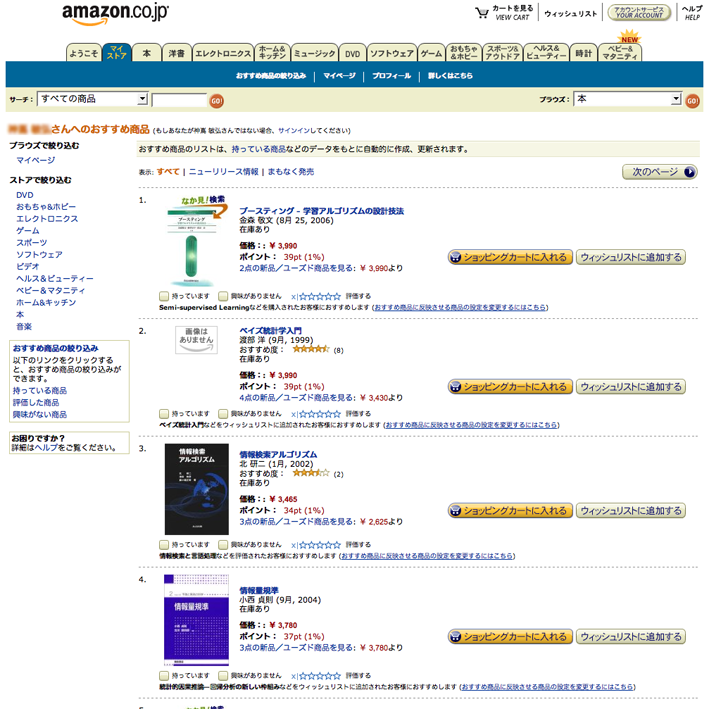
\includegraphics[width=0.48\linewidth]{pstyle1.png}}%
\hspace{0.02\linewidth}%
\subcaptionbox{評価値予測 (MovieLens~\cite{url:008})\label{fig:presentation:b}}%
{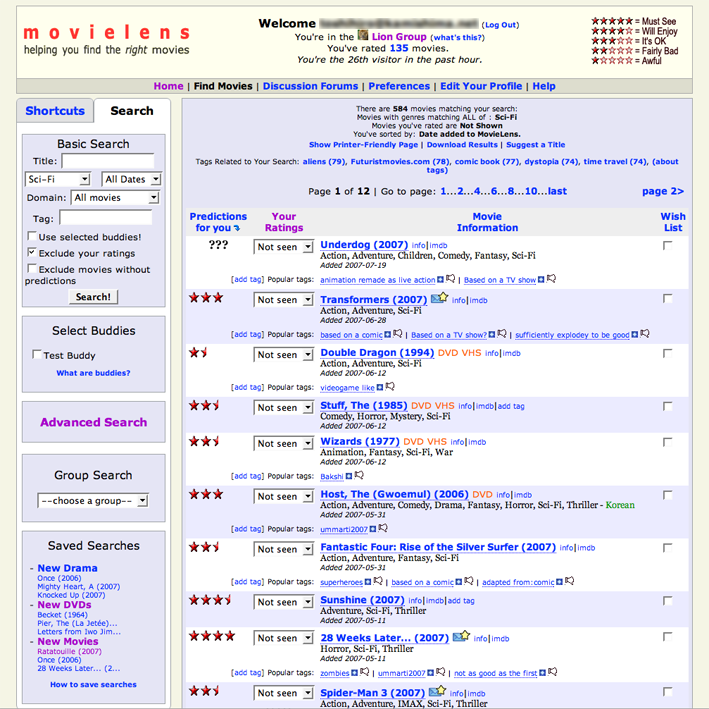
\includegraphics[width=0.48\linewidth]{pstyle2.png}}\\
\caption{推薦結果の表示例}
\label{fig:presentation}
{\footnotesize スクリーンショットは 2007/07/26 に取得した.}
\end{figure}

適合するものを一つ見つけ出す適合アイテム発見を目的とする場合には,予測される評価の高いものから順に整列したリストを利用者に提示するのが一般的である(図\ref{fig:presentation:a}).
%このリストの上位のアイテムほど,利用者の嗜好に適合する確率が高いだろう.
利用者はこのリストを上位から閲覧することで,自分の嗜好に適合したアイテムを素早く見つけることができる.

評価値予測で閲覧中にアイテムの評価を得ることを目的とする利用者は,積極的な決定をする意図をもっていない.
そこで,閲覧中のアイテムに,活動利用者の予測評価値を付随的に提示する.これは,★の数や,アイコン,グラフなどで表す(図\ref{fig:presentation:b}).
このような情報を参照することで,多数の候補の中から,利用者にとって関心のあるものを中心に閲覧できるようになる.

%利用者が自分の嗜好に適合するものを網羅的に見つけ出すことが目的である,適合アイテム列挙では,全ての候補を必ず利用者に提示しなくてはならない.

\section{多様性の向上}
\label{sec:serendipity}
\index{多様性}\index{diversity}
%@@@ 多様性の章に移行

評価値予測(\ref{sec:recomtask}節)を目的とする場合は,利用者の関心の幅を広げるため,多様性(\ref{sec:recomtype}節)の高い推薦が望まれる.
そこで,文献\cite{www:05:01}では多様性を向上させる目的で,予測精度を犠牲にしても,より広範囲の分野のアイテムを推薦する\term{話題多様化}{topic diversification}を提案している.
この多様化の有効性を,同種のアイテムに対しては,1度目より2度目,2度目より3度目に支払いたいと思う対価が減少する経済学における収穫逓減の法則 (law of diminishing marginal returns)との関連付けて論じている.
具体的には,アイテムの階層的な分類を導入し,分類階層の近さによってアイテム間の類似度を測る.
純粋に予測精度を重視したリストの上位から順に,最終推薦リストにアイテムを一つずつ追加するが,このとき,すでに推薦したアイテムと類似しているアイテムは推薦されにくいようにする.
この方法により,予測精度を犠牲にして,アイテムの多様性をより重視するような推薦をする実験を行った.
予測精度を単調に減少させ,徐々に多様性を高めると,最初は利用者は推薦の多様性の高まりを認知できたが,ある程度以上になると認知できなくなった.
よって,推薦リストの多様性を利用者が認知できる程度にとどめれば,予測精度もそれほど低下せず,利用者の満足は高まると報告している.
その他,推薦リストに,新製品やあまり知られていないアイテムを必ず混ぜるといった手法も考えられる\cite{sigir:01:01}.

\section{推薦理由}
\label{sec:explanation}
%@@@ 独立した章に

利用者は,不必要に高価なものを薦められていると疑ったりするため,推薦したアイテムを必ずしも採用するわけではない.
採用されない推薦は無意味なので,推薦ができるだけ採用されるような工夫が必要である.
そうした工夫として,アイテムの\term{推薦理由}{explanation of recommendations}も示すことが有効とされている.

文献\cite{sigchi:02:01}では,推薦の\term{透明性}{transparency}と利用者の推薦結果に与える印象との関係を調査している.
ここでいう透明性とは,利用者の入力した評価やその他の情報と,出力された推薦との間の因果関係が明確に説明されていることである.
この調査では,12人の被験者に5種類の商用音楽推薦システムを利用させた.
そして,推薦されたアイテムを好むか,推薦は信頼できるか,そして推薦に透明性があったかの質問をした.
調査の結果は,透明性があると考えた場合の方が,そうでない場合に比べて,有意に推薦された結果を好み,また,その結果を信頼できると答えた.
さらに,推薦されたアイテムを,(a)知らない場合,(b)知っていてかつそれを好きな場合,および(c)知っていてかつそれを嫌いな場合に分け
た.
推薦されたアイテムを好むかどうかの質問については,(b) (a) (c)の順に好んだ.
さらに,(a)と(b)の推薦については,推薦に透明性があると,ないときよりも,有意に推薦されたアイテムを好んだ.
しかし,(c)の推薦については,有意な差はなかった.
これらのことから,利用者が推薦に透明性があると考えたときには,推薦されたものをより好み,その推薦を信頼する.
また,知っている好きなアイテムを推薦されると,推薦に透明性があると利用者は考えるといえる.
なお,実際がどうであるかにかかわらず,透明性があると考えたかを利用者に質問した結果であること,また,システムがデータをねつ造していない点については,利用者はシステムを信頼していることには注意されたい.
利用者もおそらく知っているであろう,一般に知られたアイテムを推薦して,利用者の推薦への信頼を向上させるといったこともできる\cite{sigir:01:01}.

\begin{figure}
\centering
\subcaptionbox{類似した嗜好の利用者の評価の提示 \cite{cscw:00:01}\label{fig:explanation:a}}%
{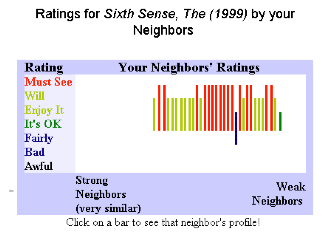
\includegraphics[width=0.48\linewidth]{Herlocker.png}}%
\hspace{0.02\linewidth}%
\subcaptionbox{推薦の根拠となった嗜好データの提示 (Amazon.co.jp)\label{fig:explanation:b}}%
{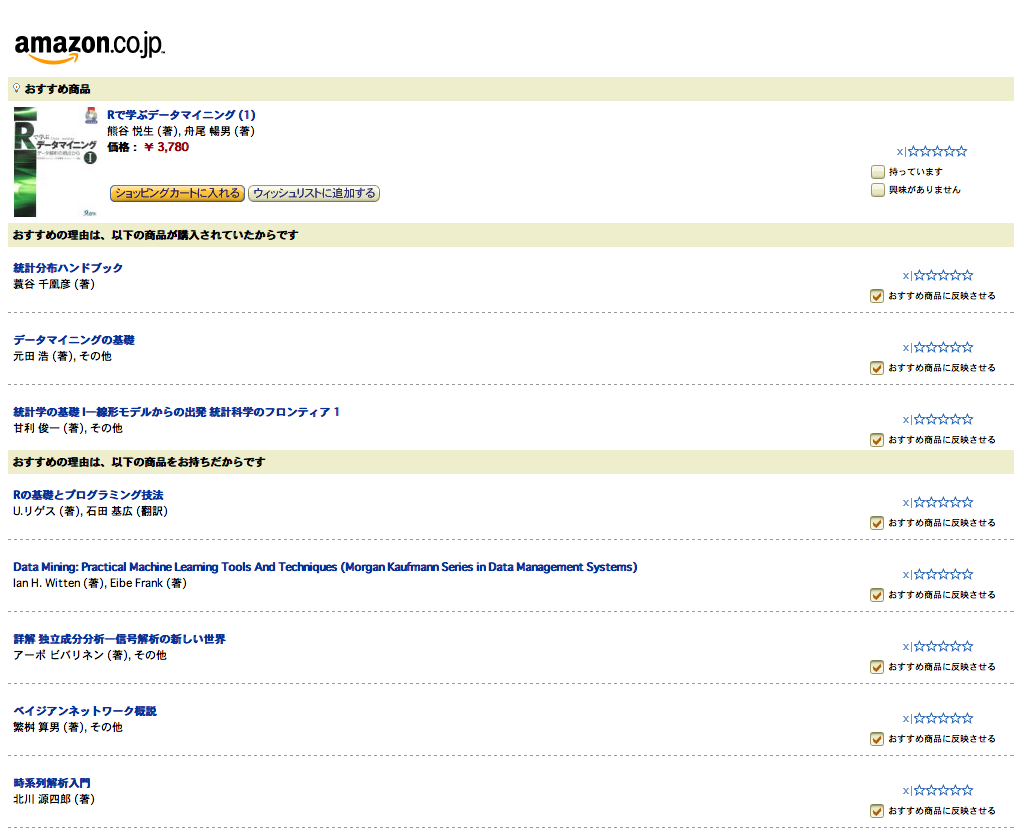
\includegraphics[width=0.48\linewidth]{explanation2.png}}\\
\caption{推薦理由の提示例}
\label{fig:explanation}
{\footnotesize スクリーンショットは 2007/07/26 に取得した.}
\end{figure}

推薦の透明性を高める,すなわち,利用者が入力した嗜好データから,推薦を導いた根拠を明示することで,推薦への信頼を高める試みがある.
文献\cite{cscw:00:01}では,こうした根拠を提示する手法を比較している.
その中で最も有効な方法とされたのが図\ref{fig:explanation:a}の方法である.
これは,活動利用者と類似した嗜好をもつ他の利用者の,推薦した映画についての評価値を棒グラフで示したものである.
この例では,推薦した映画について,嗜好が似ている人たちのほとんどが,最高か,それに次ぐ評価をしていることが,一目で分かる.
このように,推薦の手順の内部を示すアプローチを\term{ホワイトボックス}{whitebox}アプローチと呼ぶ.
その次に有効であったのは,そうした手順を示さない\term{ブラックボックス}{blackbox}アプローチの,推薦の確信度を示すことであった.
ここで,推薦の\term{強度}{strength}と\term{確信度}{confidence}について述べておこう.
推薦の強度とは,どれくらいアイテムを好むと予測しているかということである.
利用者の嗜好を5段階で予測するなら,5と予測したときに強い推薦といえる.
一方の推薦の確信度とは,この推薦をどれくらい確かだと考えているかということである.
\ref{sec:probmodel}節の確率モデルで,適合/不適合の2段階で活動利用者の嗜好を予測したとしよう.
このとき,適合すると予測した確率が$0.6$でも$0.9$でも,予測は「適合」だが,後者のときにより確かな推薦といえる.
さらに,他の方法でも実験したが,利用者の満足を向上させた方法は無かったと報告している.

その他,\ref{sec:item-item}節のようにアイテム間の類似度に基づく推薦では,推薦に関連したアイテムを提示するというホワイトボックスアプローチもある.
図\ref{fig:explanation:b}は,活動利用者自身の,推薦の根拠となった他のアイテムへの評価を提示したものである.
また,暗黙的に嗜好データを獲得した場合,推薦の根拠を利用者が認知できなくなるので,推薦と共に根拠となった嗜好データを示す方法もある.
ただし,予測評価値などを提示して,利用者が嫌いなアイテムが高評価されていると,システムに対する信頼を失う危険性も指摘されている\cite{sigir:01:01}.


\part{推薦システムのアルゴリズム}
\label{part:algorithm}
%!TEX root =  main.tex
%!TEX encoding = UTF-8 Unicode
\chapter{協調フィルタリング}
\label{chap:cf}

ここでは,協調フィルタリングによる嗜好の予測について述べる.
ここでいう予測とは,活動利用者はまだ知らないが,他の標本利用者は知っているアイテムについて,活動利用者の関心の有無や,評価値を推定することである.
このように,与えられたデータの中から,規則性を見つけ出し,その規則性に基づいて予測する問題は,機械学習や統計的予測の枠組みによって解く.
だが,万能な予測手法は理論的にありえないことは,ノーフリーランチ定理として知られている.
よって,\ref{chap:design}章で述べた,利用者数やアイテム数などのデータの特性,望ましい推薦が備えるべき性質を考慮してモデルやアルゴリズムを選択しなくてはならない.
もしこれらが適切でなければ,データがいくらあっても予測精度が向上することはないので,この選択は重要である.
これらの選択に関連した,モデルやアルゴリズムの特徴に留意して述べるので,参考にされたい.

\section{メモリベース法とモデルベース法}
\label{sec:memory-model}


個々のアルゴリズムについて述べる前に,協調フィルタリング手法の分類と,それぞれのグループの長所と短所を述べる.
推薦候補の予測手法は\term{メモリベース法}{memory-based method}(事例ベース法 (instance-based method)ともいう)と
\term{モデルベース法}{model-based method} に分けられる\cite{uai:98:01}.
\index{事例ベース法|see{メモリベース法}}\index{instance-based method|see{memory-based method}}
メモリベース法では,推薦システムが利用される以前には何もせず,ただ利用者DBを保持している.
\index{利用者データベース}\index{user database}
そして,推薦をするときに,利用者DB中の嗜好データそのものと,活動利用者の嗜好データを併せて予測をする.
もう一方のモデルベース法では,推薦システムが利用される以前に,あらかじめモデルを構築する.
このモデルは,「佐藤さんが好むものは,鈴木さんも好むことが多い」といった,利用者とアイテムの嗜好についての規則性を表す.
推薦をするときに,利用者DBは用いずに,このモデルと活動利用者の嗜好データとに基づいて予測する.
すなわち,事前にモデルを構築するかどうかという違いが重要である.

\begin{table}
\centering
\caption{メモリベース法とモデルベース法の比較}
\label{tab:memory-model}
\begin{tabular}{l@{\qquad}>{\centering}p{8zw}>{\centering}p{8zw}p{0pt}}\toprule
 & メモリベース法 & モデルベース法 & \\\midrule
推薦時間 & ×\,:\,遅い & ○\,:\,速い & \\
適応性   & ○\,:\,あり & ×\,:\,なし & \\
\bottomrule
\end{tabular}
\end{table}

これら二つの手法の大まかな長所と短所を表\ref{tab:memory-model}にまとめておく.
推薦時間についてだが,メモリベース法は一般に遅い.
これは,利用者DBには多数の標本利用者や推薦対象が登録されており,これら多数の項目を推薦の度に調べ直すのに時間がかかるためである.
一方のモデルベース法では,夜間などシステムが利用されない間や,毎月や毎週など定期的にモデルをあらかじめ構築・更新しておく.
すると,この時間は推薦の時間からは除外できる.
また,モデルの規模は,利用者DBのそれと比べて小さいので,活動利用者に速く推薦することができる.

表\ref{tab:memory-model}の適応性とは,標本利用者や推薦対象が,削除されたり追加されたりしても,適切な推薦ができるかということである.
このような削除や追加をすると,モデルベース法では,利用者や推薦対象間の規則性に変化が生じるため,モデルを再構築する必要が生じる.
だが,モデルの構築には時間がかかるので,頻繁に行うことは難しい.
そのため,適応性に関してはモデルベース法は不利になる.
一方,メモリベース法では,モデルの構築は行わないためこのような問題は生じない.

%@@@ 協調フィルタリングの形式的な定式化についてまとめる:明示的・暗黙的,ch-memorybased の一部を移してくる

%!TEX root =  main.tex
%!TEX encoding = UTF-8 Unicode
\chapter{メモリベース型協調フィルタリング}
\label{chap:memorybase}

\termmain{メモリベース法}{memory-based method}とは,利用者DBを直接利用して,活動利用者の嗜好を推定する方法である.
機械学習の観点からは$k$近傍法 ($k$-nearest neighbor method)とみなせる.
この方法は,大きく\term{利用者間型メモリベース法}{user-user memory-based method}と\term{アイテム間型メモリベース法}{item-item memory-based method}とに分類できる.
どちらも,類似性を計算する点では共通しているが,利用者間型は,活動利用者と嗜好パターンが似ている利用者をまず見つけ,彼らが好むものを推薦する.
一方,アイテム間型では,活動利用者が好むアイテムと類似したアイテムを推薦する.これらの手法を順に紹介する.

\section{利用者間型メモリベース法}
\label{sec:user-user}
\index{利用者間型メモリベース法}\index{user-user memory-based method}

利用者間型メモリベース法の代表的な手法であるGroupLensの方法\cite{cscw:94:01}について述べる.
これは,協調フィルタリングの手順を自動化した先駆的研究である.
簡潔な手法だが,その予測精度は高く,多くの改良研究もなされている.
GroupLensは,当初は NetNews の記事を推薦するシステムであったが,現在は映画の推薦システム MovieLensとなっている.
この実験システムは,プロジェクトのホームページ\cite{url:008} で公開されているので,推薦システムを体感するため利用してみてるとよいだろう.

レストランを探す場合のことを考えてみよう.
このとき,自分と食べ物の嗜好が似ている何人かの人に尋ねてみて,彼らの意見をもとにどの店で食事をするか決めたりすることがあるだろう.
GroupLensの方法は,こうした人のコミュニティでの「口コミ」による推薦の過程を,次の二段階で実現する.
\begin{description}
 \item[類似度の計算]
 利用者DB中の各標本利用者と活動利用者の嗜好の類似度を求める.
 類似度とは,嗜好パターンがどれくらい似ているかを定量化したものである.
 \item[嗜好の予測]
 活動利用者は知らないアイテムについて,それらのアイテムへの標本利用者の好みと,その標本利用者との間の類似度に基づいて,活動利用者がどれくらいそのアイテムを好むかを予測する.
\end{description}

%@@@ ch-cf  に問題の定式化の節を作成する
これらの段階について詳細に説明する前に,記号を定義する.
$n$人の全利用者の集合を$\calX=\cbr{1,\dotsc,n}$,$m$種類の全アイテムの集合を$\calY=\cbr{1,\dotsc,m}$とする.
評価値行列 $\bfR$ は利用者 $x\in\calX$ の,アイテム $y\in \calY$ への評価値$r_{xy}$ を要素とする行列である.
$r_{xy}$ は,評価済みなら評価値の定義域$\calR$のいずれかの値をとり,未評価なら欠損値「$\nan$」をとる.
例えば,5段階のスコアを用いた採点法(\ref{sec:explicitrating}節を参照)で獲得した嗜好データであれば,評価値の定義域は$\calR=\cbr{1,\dotsc,5}$となる.
活動利用者を添え字 $a$ で表す,すなわち,$r_{ay}$は活動利用者のアイテム$y$への評価値である.
また,利用者$x$が評価済みのアイテムの集合を$\calY_x=\cbr{y| y\in\calY, r_{xy}\ne\nan}$で表す.
活動利用者と利用者$i$の類似度は,共通に評価しているアイテムについてのPearson相関で測る.
\begin{equation}
\rho_{ax}=
\frac{\sum_{y\in\calY_{ax}}(r_{ay}-\bar{r}'_a)(r_{xy}-\bar{r}'_x)}%
{\sqrt{\sum_{y\in\calY_{ax}}(r_{ay}-\bar{r}'_a)^2}\sqrt{\sum_{y\in\calY_{ax}}(r_{xy}-\bar{r}'_x)^2}}
\label{eq:glsim}
\end{equation}
ただし,$\calY_{ax}$ は利用者$a$と$x$が共通に評価したアイテムの集合,すなわち,$\calY_{ax}=\calY_a\cap \calY_x$で,
${\bar{r}'}_x=\sum_{y\in \mathcal{Y}_{ax}}r_{xy}/|\calY_{ax}|$である.
なお,$|\calY_{ax}|\le1$,すなわち,活動利用者$a$と標本利用者$x$が共通に評価したアイテムが一つ以下ならば,Pearson相関は
計算できないので$\rho_{ax}=0$とする.
アイテム$y\notin\calY_a$の評価値は,式\eqref{eq:glsim}の類似度で重み付けした,各標本利用者のアイテム$y$への評価値の加重平均で予測する.
\begin{equation}
\hat{r}_{ay}=
\bar{r}_a+\frac{\sum_{x\in\calX_{y}}\rho_{ax}(r_{xy}{-}\bar{r}'_x)}{\sum_{x\in\calX_{y}}|\rho_{ax}|}
\label{eq:glscr}
\end{equation}
ただし,$\calX_y$はアイテム$j$を評価済みの利用者の集合で,$\bar{r}_{x}$は利用者$x$の全評価アイテムに対する平均評価値 $\bar{r}_x=\sum_{y\in\calY_x}r_{xy}/|\calY_x|$である.
なお,活動利用者がアイテム$y$を評価済みである$a\in\calX_y$である状況では,そもそも$\hat{r}_{ay}$の推定が不要になるので想定しなくてよい.
この式の第1項は,第2項が中間的な評価で0をとるので,それを補正するバイアス項である.
また,第2項の分子は上記の加重平均であり,分母は評価している利用者が多い,すなわち$|\calX_y|$が大きいと加重平均
が大きくなりやすい問題に対する正規化項である.
また,文献\cite{cscw:94:01}では,式\eqref{eq:glscr}の第2項のように,活動利用者と標本利用者が共に評価したアイテム$\calY_{ax}$上での評価値の平均$\bar{r}'_x$を用いている.
だが,現在のGroupLensプロジェクトでは,単純に評価済みアイテムの平均値$\bar{r}_x$を用いているとのことであり%
\footnote{J.~Riedlのメールより},また,筆者の実験でも,どちらを用いても有意な差はみられなかった.
加えて,$\bar{r}_x$の方が,活動利用者が決まる前に事前に計算できる利点があるので,実際に利用するときには$\bar{r}_x$を用いる方が良いだろう.

\begin{table}
\centering
\caption{評価値行列$\bfR$の例}
\label{tab:exrate}
 \begin{tabular}{l@{\qquad}cccc}\toprule
\makebox[5zw]{} &
  \makebox[5zw]{1\,:\,親子丼} & \makebox[5zw]{2\,:\,牛丼} &
  \makebox[5zw]{3\,:\,海鮮丼} & \makebox[5zw]{4\,:\,カツ丼} \\\hline
1\,:\,山田 & 1      & 3      & $\nan$ & 3      \\
2\,:\,田中 & $\nan$ & 1      & 3      & $\nan$ \\
3\,:\,佐藤 & 2      & 1      & 3      & 1      \\
4\,:\,鈴木 & 1      & 3      & 2      & $\nan$ \\
\bottomrule
 \end{tabular}
\end{table}

ここで簡単な例を挙げよう.
表\ref{tab:exrate}はどんぶり専門店『丼兵衛』の評価値行列$\bfR$の例である.
4人の利用者は各行に対応し,4種類のアイテム(=どんぶり)は列に対応する.
評価値は3段階の採点法,すなわち,$\calR=\cbr{1,2,3}$である.
この表は,利用者3の佐藤のアイテム2の牛丼の評価値は1で,嫌いであることを示している.
具体的に,活動利用者を田中,すなわち$a=2$とし,2\,:\,田中の1\,:\,親子丼への推定評価値$\hat{r}_{2,1}$を求めてみよう.

まず,式\eqref{eq:glsim}の相関係数を求める.
親子丼を評価済みの利用者,すなわち$\calX_1$に含まれる各利用者と活動利用者の間の相関係数を求める必要がある.
1\,:\,山田,3\,:\,佐藤,4\,:\,鈴木の3人とも親子丼を評価済みなので$\calX_1=\cbr{1,3,4}$の各利用者との相関係数を求める.
2\,:\,田中と1\,:\,山田の相関係数$\rho_{2,1}$は,共通に評価しているアイテムが2\,:\,牛丼だけで,1個以下なので$\rho_{2,1}=0$となる.
次に,2\,:\,田中と3\,:\,佐藤の間の相関係数を計算する.
この二人が共通に評価しているのアイテムは2\,:\,牛丼と3\,:\,海鮮丼なので$\calY_{2,3}=\cbr{2,3}$となる.
すると,これらのアイテムについての$\calY_{2,3}$上の平均評価値はそれぞれ
\begin{align*}
{\bar{r}'}_2 &=(\sum_{y=2,3}r_{2,y})/2=(1+3)/2=2 \\
{\bar{r}'}_3 &=(\sum_{y=2,3}r_{3,y})/2=(1+3)/2=2
\end{align*}
となり,相関係数は次式になる.
{\small\begin{align*}
\rho_{2,3}&=\frac{\sum_{y=2,3}(r_{2,y}-{\bar{r}'}_2)(r_{3,y}-{\bar{r}'}_3)}%
{\sqrt{\sum_{y=2,3}(r_{2,y}-{\bar{r}'}_2)^2}%
 \sqrt{\sum_{y=2,3}(r_{3,y}-{\bar{r}'}_3)^2}}\\
&=\frac{(1-2)(1-2)+(3-2)(3-2)}{\sqrt{(1-2)^2+(3-2)^2}\sqrt{(1-2)^2+(3-2)^2}}\\
&=1
\end{align*}}
同様に計算すると2\,:\,田中と4\,:\,鈴木の相関は$\rho_{2,4}=-1$となる.

次に推定評価値を計算する.まず,2\,:\,田中の全評価済みアイテム上の平均評価値を求める.
\[
\bar{r}_2=(\sum_{y=2,3}r_{2,y})/2=(1+3)/2=2 
\]
最後に,これまで計算した値を式\eqref{eq:glscr}に代入すると
{\small\begin{align*}
\hat{r}_{2,1}&=\bar{r}_2+
\frac{\sum_{x=1,3,4}\rho_{2,x}(r_{x,1}-{\bar{r}'}_x)}%
{\sum_{x=1,3,4}|\rho_{2,x}|} \\
&=2+\frac{0(1-3)+1(2-2)+(-1)(1-5/2)}{|0|+|1|+|-1|}\\
&=2.75
\end{align*}}
によって,2\,:\,田中の1\,:\,親子丼への推定評価値は$2.75$と計算できる.
この値は,最大値3にかなり近く,2\,:\,田中は1\,:\,親子丼が好きであると予測される.

%@@@ コサインを使った暗黙的評価の場合

\subsection{利用者間型メモリベース法の改良}

GroupLensの方法にはいろいろな改良が試みられている.
文献\cite{sigir:99:02}では,いろいろな改良を実験的に検証している.
全ての計算の前に,評価値 $r_{xy}$ から利用者$x$の平均評価値$\bar{r}_x$を引いて正規化しておくと予測精度は向上する.
これは,\ref{sec:explicitrating}節で述べたように,計測された評価値揺らぎや偏りがある.
肯定的でも否定的でもない評価値を$0$に正規化することで,こうした不整合が緩和されるためであろうと著者は考える.
利用者の近傍を使う改良もある.
ここでの近傍とは,式\eqref{eq:glsim}の相関が大きな,すなわち活動利用者と類似した嗜好をもつ利用者の集合のことである.
式\eqref{eq:glscr}の推定評価値は,アイテム$y$を評価済みの全ての利用者の評価に基づいているが,これを事前に計算した活動利用者の近傍のみに基づいて計算する.
実験によれば,近傍利用者数がある程度以上になると,それ以降は増やしても予測精度は向上しない.
よって,近傍利用者だけに計算を限定することで計算量を減らし,データベースの参照も抑制できるので,効率よく計算できるようになる.
ただし,モデルベース法のモデルほど頻繁にする必要はないが,近傍は定期的に更新しなくてはならないので,純粋なメモリベース法の利点は部分的には失われる.
また,新規の参加者については近傍を新たに計算する必要が生じ,脱退者が他の利用者の近傍利用者であれば予測精度の低下を招く.
以上の,二つの改良は,ほとんどのデータに対して有効なので,適用しておく方がよいだろう.
その他,この文献\cite{sigir:99:02}では,データが疎である問題に対処するため,活動利用者と標本利用者が共通に評価しているアイテムの数に応じて重み付けしたり,式\eqref{eq:glsim}のPearson相関の代わりに順位相関を使ったりすることは予測精度の向上に役立ったと報告している.

文献\cite{uai:98:01}にも,いくつかの改良が示されている.
その一つに,評価値の数が少ない場合に有効な\term{デフォルト投票}{default voting}がある.
利用者間の類似度は,共通に評価しているアイテム$\calY_ax$への評価に基づいて計算する.
しかし,そうしたアイテムが少ないか,全くない場合には,適切に類似度を評価できない.
例えば,利用者1と2の評価済みアイテム集合がそれぞれ$\calY_1=\cbr{1,2,3}$と$\calY_2=\cbr{1,4,5}$とする.
このとき,これら二人の類似度は共通して評価しているアイテム$1$に対する評価値$s_{1,1}$と$s_{2,1}$の二つの値だけに依存する.
このとき類似度は,共通に評価したアイテム数$|\calY_1\cap \calY_2|$は一つだけなので$0$となってしまう.
そのため,これらの利用者間の類似度は全く推薦の精度向上に寄与しない.
そこで,利用者1の$r_{1,2}$,$r_{1,3}$と,利用者2の$r_{2,4}$,$r_{2,5}$の評価値を活用する.
例えば,$r_{1,2}$の評価値は,利用者2の対応する値$r_{2,2}$があれば相関の計算に利用できる.
そこで,アイテム2の中立的な評価値,すなわち,全利用者のアイテム2への評価値の平均$\tilde{r}_y=\sum_{x\in\cal{X}_y} r_{xy}/|\calX_y|$をデフォルト投票値とし,$r_{2,2}$の値をこのデフォルト投票値で置き換える.
他のアイテムについても同様の置き換えをすると,アイテム集合$\calY_1\cup\calY_2=\cbr{1,2,3,4,5}$上でより適切に利用者間の類似度を評価できるようになる.
筆者の実験でも,一人あたりの評価値数が少ない状況でかなりの効果が確認された.
%また,$r_{xy}$の欠損を補うときに,アイテムの平均評価値$\tilde{r}_y$の代わりに,利用者$x$の全アイテム上の平均評価値$\bar{r}_x=\sum_{x\in\calYx_x}r_{xy}/|\calY_x|$も利用する実験も行ったが,あまり良い結果は得られなかった.
%しかし,どちらのデフォルト投票値が良くなるかは,データに依存するので,\ref{sec:recomtype}節の方法で予測精度を評価し,良い方を採用するとよいだろう.
この文献\cite{uai:98:01}では,最低や最高など両端に近い評価値をより重視する改良や,評価している利用者が少ないアイテムへの評価値を重視する改良などを提案している.

\ref{sec:rsyslimit}節で述べたように推薦システムが扱うデータは非常に疎である.
機械学習では,このような場合には,次元削減の前処理を実行することが多い.
代表的な方法に主成分分析\cite{eb:053:00,jpublist:077x,jb:021:00}がある.
GroupLensの方法では,各利用者は$m$個のアイテムへの評価値を要素とするベクトルで表される.
これをデータの分散に関する情報をできるだけ失わないように,$K< m$の$K$要素のベクトルで各利用者を表現するのが主成分分析である.
この$K$要素に情報を圧縮したベクトルで,利用者間の類似度を求める方法もよく用いらている\cite{ec:007,sigir:06:01}.
ただし,主成分分析は欠損値があると実行できないので,上記のデフォルト投票値やEMアルゴリズムなどによって適当に評価値行列$S$を補完する必要がある.

\section{アイテム間型メモリベース法}
\label{sec:item-item}
\index{アイテム間型メモリベース法}\index{item-item memory-based method}

GroupLensなどの利用者間型では,評価値行列$\bfR$の行ベクトル,すなわちある利用者のいろいろなアイテムへの嗜好を表すベクトルの類似度に基づいて,他の利用者の評価値を予測した.
一方,アイテム間型メモリベース法では,アイテムベクトル,すなわち,$\bfR$の列ベクトルの類似度を用いる.
これは,いろいろな人に同じような評価を受けるアイテムは似ていると考え,ある利用者が関心をもっているアイテムの類似アイテムにも,その利用者は関心をもつという仮定に基づいている.
簡単な方法としては,アイテムベクトルのコサイン\cite{ieeem:03:01}や,単純な共起性\cite{www:07:01},Pearson相関などでアイテム間の類似度を測り,利用者が閲覧中や,買い物かごに入れている,もしくは,直近の利用履歴にあるアイテムと類似しているアイテムを推薦する.
これら方法によって,協調フィルタリングの枠組みで,一時的個人化(\ref{sec:plevel}節)\index{一時的個人化}\index{ephemeral personalization}をした推薦ができる.

GroupLensの方法と同様に加重平均を使う方法としては\cite{www:01:02}がある.
この方法では,活動利用者のアイテム$y$への推定評価値を次式で求める.
\begin{equation}
\hat{r}_{ay}=
\frac{\sum_{j\in\calY_a}\rho'_{yj}r_{aj}}{\sum_{j\in\calY_a}|\rho'_{yj}|}
\label{eq:iicf}
\end{equation}
ただし,${\rho'}_{yj}$はアイテム$y$と$j$の類似度である.
この方法は文献\cite{kdd:04:11}でも利用され,アイテム間の類似度行列と活動利用者自身の評価値があれば利用者DBを参照することなく,ローカルマシンだけで推薦を計算できる.
よって,ある程度のプライバシー保護(\ref{chap:privacy}章)も実現できる.
GroupLensの方法と同様に,$\calX_a$に含まれるアイテム全てではなく,${\rho'}_{kj}$がしきい値以上の近傍に計算を限定すると,予測精度を下げることなく,式\eqref{eq:iicf}の計算を高速化できる.
だが,近傍アイテムが重要なので,公開中の映画・コンサートなどのように推薦対象のアイテムが頻繁に入れ替わる\textbf{item churn}\index{item churn}という状況では,頻繁な近傍の更新が必要になってしまう.
この方法は,評価しているアイテム数が少ない利用者には推薦が早くできる.
利用者間型より予測精度はよいとの報告もある.
しかし,理論的根拠はないが,実験的には特定のアイテムに推薦が偏る傾向が強く\cite{sigchi:06:01},多様性についてはアイテム間型は不利であるといわれている.

\section{メモリベース法に関するその他の研究}
\label{sec:other-memory-based}

\ref{sec:explicitrating}節でも述べように,利用者の評価値には一貫性が低い問題がある.
そこで,McLaughlinら\cite{sigir:04:01}は,投票された評価値を隣接した評価値に配分する信念分配 (belief distribution) を利用したGroupLens法の拡張を示した.
利用者が指定した評価値に最も大きな重みを与えると共に,その周囲の評価値にも小さな重みの評価値を与える.
例えば,評価値4を利用者が指定したとき,評価値4には$0.6$の重みで,それに隣接する評価値3や5には$0.2$の重みがあると考える.
すなわち,ファジィ理論でのメンバーシップ関数のようなものである.
しかし,この重みの分配の割合は予測精度に大きく影響するが,この割合は調整は試行錯誤によって行わなければならない問題がある.

\ref{sec:explicitrating}節では,利用者から嗜好データを得るために,採点法や格付け法ではなく順位法を用いるなんとなく協調フィルタリング\cite{epublist:039}について述べた.
ここでは,順位法で得た嗜好順序を使って推薦する方法について述べる.
手法は非常に単純で,嗜好順序中のアイテムの順位をそのまま評価値とする.例えば,利用者$x$がアイテム 1,2,3,4 を好きなものから順に$3{\succ}2{\succ}4{\succ}1$と並べた場合,アイテム4の順位は2であり,$r_{x4}=2$ として扱う.
このとき,$r_{xy}$が小さいほど好きなことを表すので,式\eqref{eq:glscr}の$\hat{r}_{ay}$ が小さいものから順に推薦する.
また,順位法では評価は常に相対的なので,予測評価値も相対的な好みしか示さないことに注意しなくてはならない.
利用者ごとに整列したアイテム数が異なる場合には,嗜好順序の長さが一定ではない.
この場合は,嗜好順序の長さを$L$とし,この嗜好順序中のアイテム$y$の順位を$\mathrm{rank}_y$としたとき,$r_{xy}=\mathrm{rank}_y(L+1)/(m+1)$とする.
これは,嗜好順序に含まれる$L$個の対象が,$m$個の全対象から一様にランダムに選ばれたとしたときの,アイテム$y$の順位の期待値である.
著者の実験\cite{epublist:064}では,採点法で得た評価値を正規化するなどしても,順位法による嗜好データに基づく予測順序の精度の方が良かった.

GroupLensの方法では,利用者間の類似度は式\eqref{eq:glsim}のPearson相関で測っている.
実験的にはこの類似度でかなり良い予測精度が得られているが,理論的な根拠は弱い.
そこで,さらに予測精度を向上させるため,経験損失を最小にするようにこの類似度関数を学習する方法\cite{kdd:07:01}もある.
これにより予測精度は向上するが,\ref{sec:memory-model}節で述べたモデルベース法と同じ適応性の問題を生じてしまう.

純粋に理論的な観点から,Pennockら\cite{aaai:00:02}は,望ましい協調フィルタリングが備えるべき公理的性質について論じた.
\index{不可能性定理}\index{impossibility theorem}
これは,社会全体での意志決定を論じる社会選択の研究で著名なArrowの不可能性定理\cite{eb:040:00}のような考え方である.
四つの公理的性質として,全定義域と最小機能(universal domain and minimal functionality),全員一致(Pareto性,unanimity),無関係な候補からの独立性(independence of irrelevant alternatives),スケール不変性(scale invariance)を挙げている.
これらの,性質を満たす予測手法は最近傍法のみであることを示している.
実際の推薦システムで,これらの公理的性質が厳密に満たされなければならないわけではないが,こうした研究は推薦システムの手法の選択指針について参考になるであろう.

%!TEX root =  main.tex
%!TEX encoding = UTF-8 Unicode
\chapter{協調フィルタリング:モデルベース法}
\label{chap:modelbase}
\indexmain{モデルベース法}\indexmain{model-based method}

モデルベース法では,活動利用者に推薦をする前にモデルを構築する.
\ref{sec:aboutarticle}で述べたように,万能なモデルは存在しないので,多様なモデルが目的に合わせて提案されている.こらを順次紹介する.

\section{クラスタモデル}
\label{sec:clustermodel}

嗜好パターンが類似している利用者が好むものを推薦するという手順を,直観的に実装したのがクラスタモデルである\cite{uai:98:01,epublist:039}.
クラスタとは対象の集合を分割した部分集合で,同じクラスタ内の対象は互いに似ているが,違うクラスタでは似ていないという条件を満たすものである.
こうしたクラスタを得る手法をクラスタリングという\cite{jpublist:034,jb:038:00,jb:020:00}.
この手法を用いて,嗜好パターンが類似している利用者のクラスタに,標本利用者の集合を分割する.
ここで,利用者間の類似度は,\ref{sec:memory-based}の式\eqref{eq:glsim}のPearson相関係数のように,いろいろなアイテムへの評
価値がどれくらい類似しているかによって測る.
活動利用者への推薦は,活動利用者と各クラスタとの類似度を調べ,最も似ているクラスタを見つける.
そして,そのクラスタ中の標本利用者の平均評価値が高いアイテムから順に活動利用者に推薦する.
この方法には,利用者集合とアイテム集合を同時に分割する共クラスタリング(co-clustering)を使う改良\cite{icdm:05:05}などがある.

このモデルでは,利用者DBを何個のクラスタに分けたかによって,推薦の質が大きく変わる.
クラスタ数を小さく設定すると,おおまかであまり個人化されていない推薦がなされる.そのため,cold-start問題に対して比較的強い.
しかし,推薦パターンの種類はたかだかクラスタ数に制限されるので,多数の嗜好データを集めても,ある程度以上に個人化された推薦はできない.
一方,クラスタ数を多くすると,スタートアップ問題\index{スタートアップ問題}\index{start-up problem}に対して弱くなるが,推薦の個人化の度合いは高まる.
また,クラスタ数が多すぎると安定したクラスタを求めるのが難しくなる問題もある.
よって目的に合わせてクラスタ数を調整する必要がある.

この方法には,実現が直観的なことに加え,モデルの構築も比較的高速であり,単純なので実装も容易であるといった利点がある.
推薦時も,各クラスタと活動利用者の類似性を調べるだけなので,計算量はクラスタ数だけに比例し,高速である.
欠点としては\term{灰色の羊問題}{gray sheep problem}~\cite{ej:048}がある.
例えば,映画の推薦を考えた場合,特定のジャンルのものだけを鑑賞する利用者はむしろ少なく,サスペンスとホラーなど複数のジャンルの映画を見るであろう.
クラスタモデルでは,利用者を特定のクラスタに分けてしまうため,こうした白でも黒でもない灰色の羊の利用者に適切な推薦ができない.
%こうした灰色の羊問題を生じない,あるアイテムが好きなら,他のアイテムはあまり好まない排他的な性質がある分野に適応すべきだろう.

\section{関数モデル}
\label{sec:funcmodel}

利用者が好きなものほど大きな値をとる効用関数(utility function)や,評価値そのものを予測する関数を用いるモデルを,本稿ではまとめて関数モデルと呼ぶ.
そして,これらのモデルの獲得を,回帰問題,クラス分類問題,および順序回帰問題に帰着させて解く.これらの手法を順次紹介する.

\subsection{回帰問題に帰着させる方法}

最初に,回帰問題に帰着させる手法から紹介する.
最も簡単な線形関数の場合を考える.
\ref{sec:item-item}の式\eqref{eq:iicf}は,詳細を無視すれば次のような線形モデルとみなせる.
\begin{equation}
\hat{r}_{ay} = \sum_j w_{yj} r_{aj}
\label{eq:itemlinear}
\end{equation}
\ref{sec:item-item}では,パラメータ$w_{yj}$はアイテム$y$と$j$の嗜好パターンの類似性を,相関係数など経験的に選んだ類似度で決めた.
しかし,与えられた評価値の集合を訓練事例として,機械学習の手法を適用すれば,もっと予測精度の高い関数を獲得できるのではないか?
この考えに従い,これらのパラメータを決める問題を\term{回帰}{regression}や\term{あてはめ}{fitting}~\cite{eb:053:00,jpublist:077x}という機械学習や統計的予測の問題に帰着させ解く.

まず,回帰モデルを,評価値行列$\bfR$行列の分解として捉えてみよう.
与えられた行列$\bfR$の未評価アイテムの部分は欠損しているが,欠損していない完全な評価値行列$\bfR^\ast$を考え,この行列を次のように分解する.
\begin{equation}
\bfR^\ast\approx \bfU^\T\bfV
\label{eq:factormodel}
\end{equation}
ここで,$\bfU$と$\bfV$の大きさは,それぞれ$K\times n$と$K\times m$である.
$\bfU$の第$x$列ベクトル$\bfu_x$は利用者$x$の特徴を,$\bfU$の第$y$列ベクトル$\bfu_y$はアイテム$y$の特徴を表している.
すると,利用者$x$へのアイテム$y$への評価値は$r^\ast_{xy}\approx\bfu_x^\T\bfy_y$のようなモデルで表される.
$\bfu_x$の要素を説明変数と,$\bfv_y$の要素をパラメータとみなせば式\eqref{eq:itemlinear}と同等のモデルであり,逆に$\bfv_y$を説明変数にすれば,式\eqref{eq:glscr}と類似したモデルとも解釈できる.
ここでもし$K$が$\max\{m,n\}$なら,近似ではなく厳密に$\bfR^{\ast}=\bfU^\T\bfV$となるように分解できる.
だがこれでは,観測データを書き写しただけで,嗜好パターンを要約したモデルとはいえない.
また,実際に観測できる評価値行列は$\bfR^\ast$ではなく,欠損のある$\bfR$である.
そこで,$K$を$K\ll m,n$に固定し,$\bfR^\ast$との期待的な損失を最小化するように,$\bfR$を$\bfU$と$\bfV$に分解することで,モデルを獲得する.

こうした分解をするには,\term{行列分解}{matrix decomposition}\index{matrix factorization|see{matrix decomposition}}の手法を用いる.
こうした手法の一つ\cite{sigir:02:01}を述べる.
%式\eqref{eq:iicf}は$m$個のアイテムへの評価で利用者を表現した
%が,因子分析では$K$個の因子(factor)で利用者を表す.
%すなわち,映画の場合であれば,個々の作品への評価ではなく,ヒュー
%マンドラマが好きだとか,ある女優が出ているといやだといった,より一
%般的な因子で利用者が記述されているようなものである.
%すると,式\eqref{eq:factormodel}で,$X$の列ベクトルは$K$個の因子で
%記述した利用者を,$Y$の列ベクトルはアイテムの$K$個の因子への関連性
%を表したものと解釈できる.
この方法では,残差$\paren{\bfR-\bfU^\T\bfV}$の各要素が正規分布に従うとしてモデル化し,観測された評価値の生成確率が高くなるように$\bfU$と$\bfV$を計算する.
この行列分解手法を\term{因子分析}{factor analysis}という.
分解ができれば,任意の利用者の任意アイテムに対する推定評価値$\hat{r}_{xy}=\bfu_x^\T \bfv_y$が計算できる.
しかし,実際の$\bfR$には欠損値があるので,文献\cite{sigir:02:01}では,これらの欠損値を潜在変数とみなしてEMアルゴリズム\cite{jrss:77:01}\index{EMアルゴリズム}\index{EM algorithm}を適用して解いている.
欠損値に対処する方法は,潜在変数以外にも,全員が必ず評価するアイテム集合を利用する,欠損値を平均値などで補完する,欠損した要素は無視して損失を計算する\cite{kdd:07:01}といった方法もある.
回帰モデルは単純なので,演算操作が複雑になるプライバシー保護協調フィルタリング(\ref{sec:privacycf})などへの適用や,カーネルを使った非線形回帰を導入して予測の向上を図るといった拡張が可能である.

次に文献\cite{kdd:99:04}の\textbf{Horting}\index{Horting}法を紹介する.
式\eqref{eq:itemlinear}のように全体を一つの線形モデルで表すと,大まかすぎて予測精度が低くなる場合がある.
そこで,嗜好が類似している利用者の間で局所的に線形モデルを構築する.
利用者$a$について,共通に評価したアイテムが十分に多い利用者$x$を見つける.
さらに,これらの利用者$x$の評価値$r_{xy}$から$\hat{r}_{ay}=\theta_{ax}r_{xy} + b_{ax}$の線形関数で,利用者$a$のスコアを高精度で予測できる利用者を選び出す.
このとき,利用者$x$は利用者$a$を予測可能といいう.
なお,$\theta_{ax}$や$b_{ax}$は,両者が共通に評価しているアイテムの評価値から計算可能である.
次に,利用者をノードとし,$x$から$a$への予測可能性を逆向きの$a$から$x$への有向辺でを示すグラフを生成しておく.
このグラフを用いて,利用者$a$のアイテム$y$への評価値を推定する.
利用者$a$から直接リンクしている利用者で,アイテム$y$を評価している利用者の集合を$\calX'_y$とする.
この集合が空でなければ,アイテム$y$への予測評価値は,$\calX'_y$中の利用者それぞれによる予測評価値の平均とする.
\[
 \hat{r}_{ay}=\frac{1}{|\calX'_y|}
\sum_{x\in\calX'_y}\theta_{ax}r_{xy} + b_{ax}
\]
もし,$\calX'_y$が空なら,リンクを2段たどり,アイテム$y$を評価している利用者集合を求め$\calX''_y$とする.この集合が
空でなければ次式で予測評価値を求める.
\[
\textstyle
 \hat{r}_{ay}=\frac{1}{|{\calX''}_y|}\sum_{x\in\calX''_y}\theta_{ax'}(\theta_{x'x}r_{xy} + b_{x'x}) + b_{ax'} 
\]
ただし,$x'$は,各$x$について$x$と$a$を中継する利用者である.
さらに$\calX''_y$も空ならば,3段以上のリンクを考慮する.

\subsection{クラス分類問題に帰着させる方法}

回帰と並ぶ代表的な機械学習の枠組みである\term{クラス分類}{classification}も利用できる.
アイテム$y$への評価値$r_{ax}$は,$\calR$中の値の一つをとるので,その大小関係を無視すれば,クラスと考えることができる.
また,分類するアイテム$y$の特徴量には,このアイテムへの他の利用者による評価値や,活動利用者の他のアイテムへの評価値が利用できる.
あとは,これらの特徴量で表されたアイテムが分類されるべきクラス,すなわち評価値を予測するモデルをクラス分類の学習手法によって獲得すればよい.

このような方法として,\term{逐次型二項関係学習法}{Cross-G-Learn-Relation method}\cite{icml:98:01,jb:032:04}を紹介する.
なお,原論文では評価大小関係を考慮する工夫がさらになされているが,ここでは簡潔に記す.
これは,各クラスごとに,対象の分類されやすさを表す関数を獲得し,その関数の値が最大になるクラスに対象を分類する.
利用者$x$のアイテム$y$の評価値を予測するとき,逐次型二項関係学習法では,アイテム$y$への他の利用者の評価と,利用者$x$のその他のアイテムへの評価を入力とした次の関数を用いる
\begin{equation}
\hat{r}_{xy}=\arg\max_{r\in \calR}
\paren{\sum_{i\st r_{iy}=r}v_{xi}+\sum_{j\st r_{xj}=r}w_{yj}}
\label{eq:cglr}
\end{equation}
利用者$x$が仮にアイテム$y$の評価値を$r$としたとき,
第1項ではアイテム$y$についての評価が同じ$r$である利用者$i$について,利用者間重み$v_{xi}$の総和を求める.
同様に,第2項では利用者$x$が同じ$r$と評価をしているアイテム$j$について,アイテム間重み$w_{yj}$の総和を求める.
すなわち,類似利用者と類似アイテムの評価値の両方を考慮している.
重み$v_{xi}$と$w_{yj}$は\term{オンライン学習}{online learning}\cite{jjsai:99:02}の枠組みで求める.
これは,行列$\bfR$の形式で評価値がまとめて与えられてから学習するのではなく,誰かが何かアイテムを評価して,$r_{xy}$が一つ与えられるごとに重みをより適切なものに更新する方法である.
各評価値を与えられるごとに,予測値とその与えられた値とを比較することを繰り返し,ある時点までの累積の誤りを小さくするようにモデルを学習する.
もう少し詳しく述べると,最初に全ての重み$v_{xi}$と$w_{yj}$を初期化する.
その後,$r_{xy}$が観測されるたびに,利用者$x$以外でアイテム$y$を評価済みの全ての利用者$i$について,$r_{xy}=r_{iy}$なら重み$v_{xi}$を増やし,そうでないなら減らす.
さらに,利用者$x$が評価している$y$以外の全てのアイテム$j$について,評価値が一致すればやはり重み$w_{yj}$を増やし,そうでなければ減らす.
このように評価値が与えられるごとに重みを更新する.
この方法はオンライン学習なので,モデルベースだが,アイテムや利用者が追加されても対応できる特徴がある.
ただし,アイテムや利用者の削除には対応できない.

\subsection{順序回帰問題に帰着させる方法}

\ref{sec:explicitrating}では,採点法や格付け法による評価値は,本来は順序付カテゴリとして扱うべきものであることを述べた.
すなわち,評価値が2のアイテムは,4のアイテムの半分程度好きなのではなく,評価値3のアイテムより,4のアイテムの方がより好きであるということだけを示している.
こうした順序付カテゴリ値を予測する問題は順序回帰と呼ばれる.
この順序回帰を,ブースティング (boosting) \cite{icml:96:02,jjsai:99:01} の枠組みで扱う\textbf{RankBoost}~\cite{icml:98:03,jmlr:03:02} \index{rankboost@RankBoost}で推薦をする研究などがある.
後に,この順序回帰を用いた,内容ベースと協調フィルタリングのハイブリッド法を\ref{sec:combmethod}で紹介する.

\section{確率モデル}
\label{sec:probmodel}

モデル化に用いた関数が確率分布として解釈できるものを本稿では特に確率モデルと呼ぶ.
これら確率モデルを,大きく履歴条件型と共起型の二つに分け,順に説明する.

\subsection{履歴条件型}

履歴条件型の確率モデルでは,活動利用者のアイテム$j$への評価値を次の条件付期待値で予測する\cite{uai:98:01}.
\begin{align}
\hat{r}_{ay} & = \expect\bra{r_{ay}|r_{aj}\st j\in\calY_a}\nonumber\\
& = \sum_{r\in\calR} r\;\pb{r_{ay}=r|r_{aj}\st j\in\calY_a}
\label{eq:escoreg}
\end{align}
これは,活動利用者の過去の嗜好データが与えられたときの,活動利用者のアイテム$y$への評価値の条件付期待値である.
実際には,式\eqref{eq:escoreg}中の確率分布は未知なので,推定した関数を利用する.
式中では他の標本利用者の嗜好データが参照されていないが,確率分布の推定の過程で,これらの嗜好データを利用するため,協調フィルタリングによる推薦といえる.
また,適合/不適合の2値の嗜好データ,すなわち$\calR=\cbr{0,1}$の場合,式
\eqref{eq:escoreg}は単なる条件付確率分布となる.
\begin{equation}
\hat{r}_{ay}=\pb{r_{ay}=1|s_{aj}\st j\in \calY_a}
\label{eq:escore}
\end{equation}
このように簡潔になるので,予測評価値を提示する評価閲覧よりも,適合か不適合かの判定ができればよい適合アイテム発見タスクに適す.
\index{適合アイテム発見}\index{finding some good items}
この履歴条件型モデルでは,条件付確率\eqref{eq:escore}の計算のため,肯定的評価の$r_{xy}=1$と否定的評価の$r_{xy}=0$の両方の場合の訓練事例が必要である.
しかし,\ref{sec:getpref}で述べたように,暗黙的な評価では,購入や閲覧などの行動がなかったことで否定的な評価とみなす.
すると,未評価と否定的評価は混同され,$r_{xy}=0$となる事例にはノイズが多くなる.
そのため,未評価と否定的評価が明確に区別される事例が必要となり,な,この履歴条件型ではこうした暗黙的評価では不利になる.

式\eqref{eq:escoreg}中の条件付確率は,$\calY_a$に依存するため,各利用者について個々にモデルを獲得する必要が生じ,実用的ではない.
そこで実際には,利用者には依存しない,次の全アイテムへの評価の同時分布を求める.
\begin{equation}
\Pr[r_{\cdot y}\st y\in \calY]
\label{eq:jprob}
\end{equation}
そして,式\eqref{eq:escoreg}中の条件付分布は,ベイズ則と不要な変数を周辺化で消去することで計算する.
だが,各$r_{\cdot y}$は$|\calR|$個の値をとることが可能で$|\calY|=m$なので,この分布の定義域は$\calR^{\calY}=\calR_{1}\times\calR_{2}\times\cdots\times\calR_{m}$である.
よって,この分布の飽和モデルのパラメータ数は$|\mathcal{R}|^m-1$となり,$m$に対して指数的に増加する.
しかし,データは疎で$m$は大きいので,単純に評価値の各組み合わせの頻度を数え上げて,この飽和モデルのパラメータを推定することは現実的ではない.
そこで,このような場合の一般的な対策を導入し,変数$r_{\cdot y}$の間に部分的な条件付独立性を仮定し学習すべきパラメータ数を減らす.
このような条件付独立性を導入した確率モデルを,依存関係をグラフで表現して示すため,一般にグラフィカルモデルという.
\index{グラフィカルモデル}\index{graphical model}
その一つである\term{ベイジアンネットワーク}{Bayesian network}\cite{jb:037:00}は\cite{uai:98:01}で利用されている.
ベイジアンネット全般の問題として独立性の構造をうまく設計する難しさがあるが,うまく設計できれば学習も,推薦も効率的に実行できる.
また,式\eqref{eq:escoreg}の条件付確率を直接内部構造としてもつ確率モデルである\textbf{依存性ネットワーク (dependency network) }を使う\cite{jmlr:00:01}などもある.
このモデルでは,同時確率から条件付確率へ変換が不要なので,実行時の推薦は高速に実行できるが,事前のモデル学習の計算量は増える.

\subsection{共起型}

もう一方の共起型の確率モデルについて述べる.
このモデルでは,ある利用者が,あるアイテムを評価したことを,その利用者が$x$であるという事象と,そのアイテムが$y$であるという事象が共起しているととらえる.
そして,この共起確率をモデル化する.
このモデル化には,自然言語処理で文書と語の共起確率を表すために考案された\textbf{確率的潜在意味解析 (probabilistic latent semantic analysis; pLSA)}~\cite{uai:99:01}\indexmain{pLSA}\index{確率的潜在意味分析|see{pLSA}}\index{probabilistic latent semantic analysis|see{pLSA}}を利用する.
この確率モデルは非常に柔軟で,純粋な協調フィルタリングだけでなく,評価の揺らぎ,アイテムの特徴,コンテキスト,デモグラフィックな要因を導入するといった拡張が可能である.

本節では,利用者の嗜好データのみに基づく協調フィルタリングを対象としたモデル\cite{ijcai:99:01}を紹介する.
最初に,利用者とアイテムの共起関係だけを使うモデルについて述べる.
利用者とアイテムに対し,それぞれ$\calX=\cbr{1,\ldots,n}$と$\calY=\cbr{1,\ldots,m}$中のいずれかの値を取る多値の確率変数$X$と$Y$を割り当てる.
嗜好データを,利用者$x$がアイテム$y$を購入するという行為で暗黙的に獲得する場合を考える.
これは,$X=x$という事象と,$Y=y$という事象が共起していることに相当する.
また,$\calR=\cbr{0,1}$であるとき,$r_{xy}=1$となる対$(x,y)$が観測されることとも等価である.
履歴条件型の確率モデルでは$r_{xy}=0$となる事例も必要であったが,共起型では$r_{xy}=1$となる事例だけでモデルが学習できる.
このため,未評価と不支持が区別できない暗黙的評価の場合に,この共起型確率モデルは便利である.

さらに,このモデルで重要な役割をはたす\term{潜在変数}{latent variable} $Z$(\textbf{隠れ変数 (hidden variable)} ともいう)を導入する.
\index{隠れ変数|see{潜在変数}}\index{hidden variable|see{latent variable}}
これも多値変数で$\calZ=\cbr{1,\ldots,K}$中の値をとり,潜在的な嗜好のパターンを表す.
この潜在変数の値はデータとして観測されることはなく,モデルの中でのみその存在を仮定する.
これはクラスタモデルと類似しているので,灰色の羊問題(\ref{sec:clustermodel})\index{灰色の羊問題}\index{gray sheep problem}が生じるように思える.
だが,$K$個のパターンのうちどれか一つに割り当てるのではなく,それらが混ざり合った状態を考慮するので,この問題は生じない.
そして,この潜在変数を用いて,$x$と$y$の同時確率を,次式で表すのがpLSAモデルである.
\begin{align}
 \pb{x,y}& = \sum_{z\in \calZ}\pb{x}\pb{z|x}\pb{y|z}\label{eq:origplsamodel}\\
& = \sum_{z\in \calZ}\pb{x|z}\pb{y|z}\pb{z}
\label{eq:plsamodel}
\end{align}
このモデルでは,$z$が与えられたときに$x$と$y$が条件付独立であることを仮定して,モデルのパラメータの総数を減らしている.
また,$\pb{x|z}$,$\pb{y|z}$,$\pb{z}$はそれぞれカテゴリ分布に従う.

\begin{figure}
\centering
\begin{minipage}{0.3\fullwidth}
\centering
\setlength{\fboxsep}{0pt}
\fbox{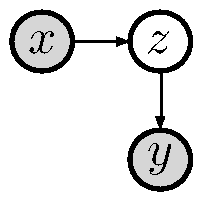
\includegraphics[width=\textwidth]{plsa.pdf}}\\
(a) 評価値なし
\end{minipage}
\hspace{0.02\fullwidth}
\begin{minipage}{0.3\fullwidth}
\centering
\setlength{\fboxsep}{0pt}
\fbox{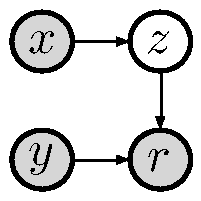
\includegraphics[width=\textwidth]{plsa2.pdf}}\\
(b) 評価値あり
\end{minipage}
\caption{pLSAモデル\cite{ijcai:99:01}}
\label{fig:latentmodel}
\end{figure}

図\ref{fig:latentmodel}(a)は,\termmain{グラフィカルモデル}{graphical model} という表現方法でpLSAモデルを図示したものである.
このグラフで,灰色のノードは値が観測される$X$や$Y$のような\term{観測変数}{observed variable}(\textbf{可視変数 (visible variable)} ともいう)を,白いノードはその値が観測されない潜在変数を表す.
\index{可視変数|see{観測変数}}\index{visible variable|see{observed variable}}
有向辺は確率的な依存関係を表し,辺が出ている変数に,辺が入っている変数が依存することを表す.
また,この図にはないが,値が確定しているパラメータは黒い点で表し,同じ確率変数を複数回サンプリングすることを示すプレートという表現もある.
これらの表現については教科書\cite[8章]{jpublist:077x}などを参考にされたい.

モデルのパラメータは$\bfTheta = \paren{\cbr{\pb{x|z}}, \cbr{\pb{y|z}},\cbr{\pb{z}}}$であるが,これらを最尤推定で求める.
すなわち,いろいろな利用者がいろいろなアイテムを評価した,$N$個のデータ$\calD=\cbr{(x_i,y_i)}_{i=1}^N$に対する次の対数尤度を最大にするように求める.
\[
\pb{\calD; \bfTheta} = \sum_{(x,y)\in \calD} \ln\pb{X=x, Y=y; \bfTheta}
\]
潜在変数があるため,この最尤推定は\termmain{EMアルゴリズム}{EM algorithm}\cite{jrss:77:01,jpublist:077x}によって行う.
具体的には次の二つのステップを交互に反復する.
一つ目のEステップでは,パラメータ$\cbr{\pb{z|x}},\cbr{\pb{y|z}},\cbr{\pb{z}}$が与えられたときの,潜在変数
の分布を求める.
\begin{equation}
\pb{z|x,y}=\frac{\pb{z}\pb{x|z}\pb{y|z}}{\sum_{z'}\pb{z'}\pb{x|z'}\pb{y|z'}}
\label{eq:estep}
\end{equation}
二つ目のMステップでは,前のステップで求めた分布$\pb{z|x,y}$を用いてパラメータを更新する.
\begin{align}
\pb{x|z} & = \frac{\sum_y n\paren{x,y} \pb{z|x,y}}{\sum_{x',y}n(x',y)\pb{z|x',y}}\label{eq:mstepx}\\
\pb{y|z} & = \frac{\sum_x n(x,y) \pb{z|x,y}}{\sum_{x,y'} n(x,y') \pb{z|x,y'}}\label{eq:mstepy}\\
\pb{z} &=\frac{\sum_{x,y}n(x,y)\pb{z|x,y}}{N}\label{eq:mstepz}
\end{align}
ただし,$n(x,y)$は,$x$と$y$が共起している$\calD$中の対の数である.
以上の手続きを収束するまで反復すると,パラメータが計算できる.
そして,次式の$\pb{y|x}$を求めておき,
\begin{equation}
\pb{y|x} = \frac{\sum_z\pb{x|z} \pb{y|z} \pb{z}}{\sum_{y',z}\pb{x|z} \pb{y'|z} \pb{z}}
\end{equation}
活動利用者$a$がアイテム$y$を好む度合いは$\pb{Y=yj|X=a}$の大きさで測る.
活動利用者$a$に対しては,この度合いを最大化する次のアイテム$y^\ast$を推薦すればよい.
\begin{equation}
y^\ast=\arg\max_{y\in\cbr{\calY\backslash\calY_{a}}}\Pr[Y=y|X=a]
\end{equation}
なおpLSAでは訓練データ中に現れない利用者,すなわち,$a\notin\calX$の場合にはこの方法では推薦できない.
このような新規利用者を扱うことを情報検索の文脈ではfolding-in\index{folding-in}という.
このfolding-inを行う方法として,潜在変数とアイテムしか現れないパラメータはそのまま固定し,利用者が関連するパラメータ$\pb{x|z}$のみを更新する手続きが提案されている\cite{misc:089}.

次に,利用者$X$とアイテム$Y$に,評価値を表す確率変数$R$も加えた拡張を考える.
この変数は,評価値の値域$\calR$中の値をとる多値変数である.
このモデル化では$X=x$,$Y=y$,および$R=r$の共起確率$\pb{x,y,r}$を扱う.
そして,利用者$a$のアイテム$y$の推定評価値$\hat{r}_{xy}$は最頻値
\[
\hat{r}_{xy}=\arg\max_{r\in\calR}\Pr[R=r|X=a,Y=y]
\]
や期待値
\[
\hat{r}_{xy}=\frac{1}{\abs{\calR}}\sum_{r\in\calR}r\;\pb{R=r|X=a,Y=y}
\]
で計算する.なお,$\pb{r|x,y}$は$\pb{x,y,r}$から計算できる.
図\ref{fig:latentmodel}(b)は$\Pr[x,y,r]$のモデル化の一例である.
このモデルでは,利用者$x$は$z$で表されるグループに分類され,そのグループ$z$とアイテム$y$に依存して評価値$r$が決まると解釈できる.
モデルを決めれば,あとは対数尤度を最大化するパラメータをEMアルゴリズムで求めればよい.
文献\cite{ijcai:99:01}では他にもいくつかのモデルを挙げている.
これらのモデルは評価値を離散変数で表し,カテゴリ分布に従うと考えているので,評価値の大小関係を無視している.
そこで離散の評価値を実数値として扱うことで大小関係を考慮し,それがガウス分布に従うとするモデルもある\cite{sigir:03:01}.
どのモデルが適切かだが,一般には\ref{sec:recomtype}で述べた交差確認法で,予測精度を最大にするようなものを選ぶ.

\begin{figure}
\centering
\begin{minipage}[t]{0.3\fullwidth}
\centering
\setlength{\fboxsep}{0pt}
\fbox{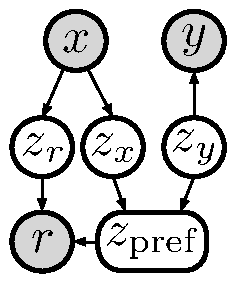
\includegraphics[width=\textwidth]{decoupled.pdf}}\\
(a) decoupled
\end{minipage}
\hspace{0.02\fullwidth}
\begin{minipage}[t]{0.3\fullwidth}
\centering
\setlength{\fboxsep}{0pt}
\fbox{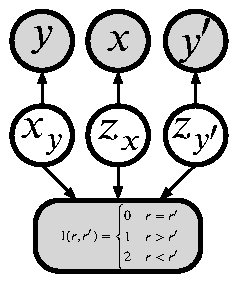
\includegraphics[width=\textwidth]{preford.pdf}}\\
(b) preferred ordering
\end{minipage}
\caption{評価値の揺らぎを考慮したモデル\cite{uai:03:01}}
\label{fig:decoupledmodel}
\end{figure}

この共起型の確率モデルは自由に設計できる余地が多く,いろいろな拡張が可能である.
\ref{sec:explicitrating}では,利用者の評価値に一貫性はなく揺らぎがあるとを述べた.
こうした揺らぎを考慮する2種類の方法を,文献\cite{uai:03:01}では提案している.
\ref{fig:decoupledmodel}(a)のdecoupledは,まず揺らぎのない真の評価値は分からないので,これを潜在変数$z_\mathrm{pref}$で表す.
\index{decoupled model}
この真の評価値は,同じ嗜好の利用者のグループを示す$z_x$と,類似したアイテムのグループを表す$z_y$に依存して決まる.
さらに,評価値がどのように揺らぐのかというパターンに利用者は分けられ,そのパターンを潜在変数$z_r$で表す.
観測される評価値$r$は真の嗜好$z_\mathrm{pref}$と揺らぎのパターン$z_r$に依存して決まる.
推薦は,予測した真の評価値$z_\mathrm{pref}$によって行う.
もう一つのpreferred orderingモデル(\ref{fig:decoupledmodel}(b))は,評価値を順序尺度と考える方法である.
\index{preferred ordering model}
同じ利用者$x$が二つのアイテム$y$と$y'$のそれぞれに$r$と$r'$の評価値を与えた場合を考える.
このとき,$r$と$r'$の順序関係だけを取り出す関数$\ind(r,r')$を導入し,この関数$\ind$の値が,利用者とアイテムのグループを表す潜在変数$z_x$と$z_y$に依存するというモデル化である.
このようにモデルを決めれば,あとはEMアルゴリズムでパラメータを学習できる.
これらのモデルでは揺らぎを扱うことができるが,パラメータの総数は増えるので,それに応じた十分な嗜好データが必要になる.

\begin{figure}
\centering
\fbox{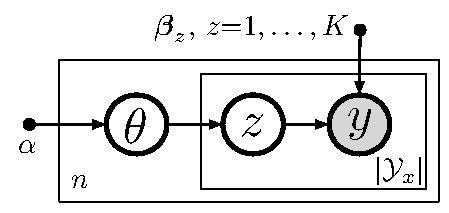
\includegraphics[width=0.6\fullwidth]{lda.pdf}}\\
\caption{潜在的ディリクレ配分法 (LDA) のモデル\cite{jmlr:03:05}}
\label{fig:lda}
\end{figure}

pLSAでは新規の利用者に対応できない問題があったが,これにベイズの枠組に拡張することで対応する\textbf{潜在的ディリクレ配分法 (latent Dirichlet allocation; LDA)}~\cite{jmlr:03:05}がある.
\index{LDA}\index{潜在的ディリクレ配分法|see{LDA}}\index{latent Dirichlet allocation|see{LDA}}
式\eqref{eq:origplsamodel}のpLSAモデルでは,最初に既知の利用者を$\calX$の中から$\pb{x}$に従って選択し,その利用者の嗜好パターンの分布$\pb{z|x}$に基づいて選んだ嗜好パターンに基づいてアイテムを選択する.
そのため,訓練データに表れない利用者については,その嗜好パターンが不明であり,pLSAでは対応できない.
そこで,嗜好パターン$\bftheta$自体をディリクレ分布に従って生成するように拡張することで,新規利用者に対応できるようにしたのがこのLDAである.
このLDAでは,訓練データ中の利用者$x$は,
しかし,変分ベイズやMCMCを用いた近似計算が必要になり,pLSAより計算量は増大する.
このLDAと類似したモデルとして\cite{icml:04:07}などもある.
%@@@ LDAについてもっと詳しく

%@@@ www:07:01 のMapReduceを用いた実装について

\section{時系列モデル}
\label{sec:timeseries}
\index{時系列}\index{time series}

時間に伴う変化を嗜好の予測に利用する方法を紹介する.
\ref{sec:getprefother}で述べたように,標本利用者の時間順の行動や評価の履歴情報を,利用者DBに蓄積している場合がある.
この情報から,利用者の行動の時間的推移を表すモデルを構築し,活動利用者の現在にいたる行動や評価とこのモデルから,嗜好を予測する手法を紹介する.

\subsection{基本的な時系列モデル}

レンタルビデオ店で,先々週はあるドラマの第1話を,先週はこのドラマの第2話を借りていった顧客がいたとする.
このとき,今週はこのドラマの第3話を借りるだろうことは容易に予測できる.
この購入履歴に基づくモデルを利用した文献\cite{nips:03:03}の方法を紹介する.
利用者が$t$回目に購入したアイテムを$y^{(t)}$で表すと,購入履歴の系列は$\ang{Y^{(t)}}=\ang{y^{(1)},y^{(2)},\ldots,y^{(t)}}$となる.
例えば,上記の連続ドラマの例であれば$y^{(1)}$〜$y^{(3)}$は,それぞれドラマの第1〜3回に相当する.
この購入履歴が与えられたときの,次に購入するアイテムの条件付確率$\pb{y^{(t+1)}|\ang{Y^{(t)}}}$を求めておき,この確率を最大にするアイテムを推薦する手法を考える.
これは,標本利用者の購入履歴を数え上げれば原理的には計算可能である.
しかし,\ref{sec:rsyslimit}で述べたようにデータが疎であるので,いたるところで確率が$0$となり,実際にはこの方法では計算できない.
このような場合には,$K$回前までの状態,すなわち購入アイテムに基づく$K$重マルコフモデルを用いることが多い.
しかし,推薦の場合にはかなり過去の情報も次の状態に影響するため,単純にこのモデルを適用してもあまり有効ではない.

そこで,自然言語処理の言語モデルでよく利用される\textbf{最大エントロピーモデル (maximum entropy model; MaxEnt model)}を導入する.
\indexmain{最大エントロピーモデル}\index{MaxEntモデル|see{最大エントロピーモデル}}
\indexmain{maximum entropy model}\index{Maxent model}
\begin{equation}
\pb{y^{(t+1)}|\ang{Y^{(t)}}}=
\frac{1}{Z}
\exp\bra{\sum_{k=1}^K\lambda_k f_k\paren{y^{(t+1)},\ang{Y^{(t)}}}}
\label{eq:maxent}
\end{equation}
ただし,$Z$は正規化定数,$\lambda_k$は重みパラメータである.
ここで\term{素性関数}{feature function} $f_k\paren{y^{(t+1)},\ang{Y^{(t)}}}$が重要になる.
素性関数は購入履歴$\ang{Y^{(t)}}$にある特徴があるとき,次回に購入するアイテムがある特定のものになるなら$1$をとり,それ以外
では$0$となるような関数である.
例えば,上記のドラマの場合,購入履歴にドラマの第2回が含まれていて,次回購入がドラマの第3回なら$1$になる関数である.
このような素性関数をtriggerと呼ぶ.
このtriggerには,購入履歴中にアイテム$y$があるときに,次回にアイテム$y'$を購入する確率
$\pb{y^{(t+1)}=y'|y\in \ang{Y^{(t)}}}$と$\pb{y^{(t+1)}=y'}$との差が大きなものを選ぶ.
こうして素数関数を選択すれば,式\eqref{eq:maxent}のモデルのパラメータ$\lambda_k$は最大エントロピー原理\cite{jb:031:00}に基づいて推定できる.
素性関数には,trigger以外にも,いろいろなものが利用できる.
次に購入するアイテムが,$s\in{0,1,2,\ldots}$個前に購入したアイテムに依存して決まるgapマルコフモデルを素性として利用する方法\cite{trieice:07:01}.
利用者自身のデモグラフィックな特徴を考慮するのも有効であろう.
系列パターンマイニング\cite{eb:044:00,icde:01:02}などと組み合わせれば,triggerよりも複雑なパターンも素性関数として利用できるだろう.

\subsection{マルコフ決定過程モデル}

\begin{figure}
\centering
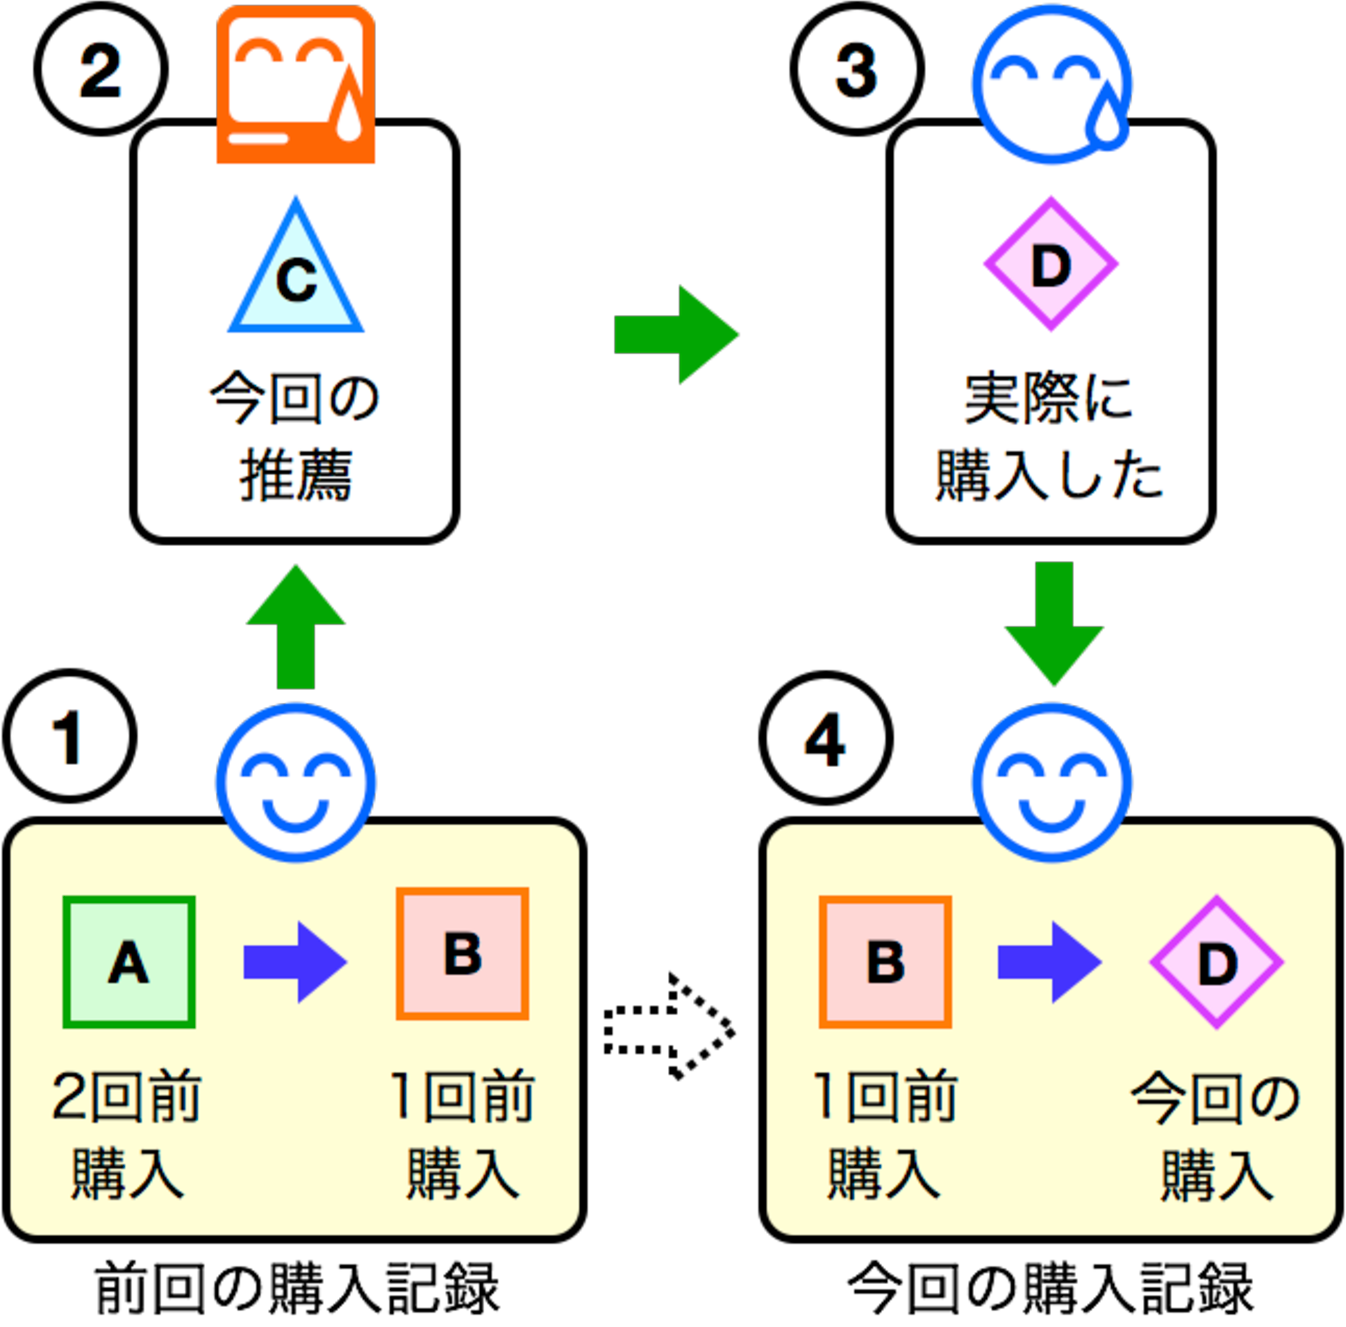
\includegraphics[width=0.6\fullwidth]{mdp.pdf}
\caption{マルコフ決定過程によるモデル}
\label{fig:mdpmodel}
\end{figure}

前節のモデルでは,過去の履歴に基づいて,次に利用者が選択する確率が最も高いアイテムを推薦する.
だが,推薦がなければそのアイテムを買ったかもしれないが,推薦の影響によってそのアイテムを選ばないという場合もある.
加えて,1年間全体で見て,選択したアイテムの価格の総和を最大化するとか,選択したアイテムへの利用者の評価の総和を最大にするような推薦をしたいとする.
これらの目的を達成するため,\term{マルコフ決定過程}{Markov decision process}を使う手法が提案されている\cite{uai:02:02,jmlr:05:03}.

マルコフ決定過程の前に\term{マルコフ過程}{Markov process}について述べる.
この過程では,次に選択するアイテム$y^{(t+1)}$は,直前の$K$個のアイテム系列$\ang{Y^{(t)}}=\ang{y^{(t-K+1)},\ldots,y^{(t)}}$に依存する.
このアイテム系列で状態を表し,状態の遷移確率は$\mathrm{tr}_\mathrm{MC}(\langle Y^{(t)}\rangle,\langle Y^{(t+1)}\rangle)$と記す.
この確率は,十分なデータがあれば,利用者の購買履歴を数え上げれば計算できる.
しかし,データは疎なので,文献\cite{uai:02:02,jmlr:05:03}ではskippingや,アイテムのクラスタリングなどの手法を用いて対処している.

次にマルコフ決定過程を図\ref{fig:mdpmodel}を用いて説明する.
図中\ajMaru{1}は現在の状態$\ang{Y^{(t)}}=\ang{y^{(t-1)}=A,y^{(t)}=B}$で,この時刻$t$にアイテムDを購入
して,図中\ajMaru{4}の次の状態$\ang{Y^{(t+1)}}=\ang{y^{(t)}=B,y^{(t+1)}=D}$に移る.
ここで,単に$\ang{Y^{(t)}}$のみに依存して$\ang{Y^{(t+1)}}$が決まる(図の点線矢印)ならマルコフ過程である.
それとは異なり,マルコフ決定過程では,状態$\ang{Y^{(t)}}$で行う推薦という行動(action)を明示的に考慮する.
これにより,推薦という行動によって,利用者の選択が変わることをモデル化できる.
この時刻$t$での行動$A^{(t)}$は図中\ajMaru{2}にあたり,アイテム$C$を推薦した.
利用者は$\ang{Y^{(t)}}$と$A^{(t)}$に依存して,アイテム$y^{(t+1)}$を選択し,次の状態$\ang{Y^{(t+1)}}$に遷移する.
図の例では,推薦を受け入れず利用者は\ajMaru{3}でアイテムDを購入したので,遷移した状態は\textcircled{\small 4}の$\ang{Y^{(t+1)}}=\ang{B,D}$となった.
この状態遷移を$\paren{\ang{Y^{(t)}},A^{(t)},\ang{Y^{(t+1)}}}$と,この遷移確率を$\Pr_\mathrm{MDP}\bra{\ang{Y^{(t)}},A^{(t)},\ang{Y^{(t+1)}}}$と記す.
また,状態$\ang{Y^{(t)}}$で行動$A^{(t)}$を決定する手続きを方策 (policy) と呼ぶ.
さらに,図の\ajMaru{3}にてアイテムDを選択したが,これに依存して報酬 (reward) が発生する.
この報酬は,アイテムへの代金や,利用者のアイテムへの評価値などである.
報酬の導入により,個別の推薦ごとの効用を最大化するのではなく,複数の推薦を含む長期間の効用の最大化を考慮できるようになる.
この報酬を最大化するような政策を決める学習問題は\term{強化学習}{reinforcement learning}\cite{eb:058:00,jb:019:00}と呼ばれる.
既存の強化学習の方法を用いて,適切な政策が獲得できれば,推薦は政策に従うことで実行可能になる.
ただし,データが疎である問題に対処するため,マルコフ決定過程の遷移確率$\Pr_\mathrm{MDP}\bra{\ang{Y^{(t)}}, A^{(t)},\ang{Y^{(t+1)}}}$を,マルコフ過程の遷移確率$\Pr_\mathrm{MC}\bra{\ang{Y^{(t)}}, \ang{Y^{(t+1)}}}$によって初期
化するなどのヒューリスティックを用いている.

\subsection{定期購入サービス}

時系列を扱う手法の最後に\term{定期購入}{subscription}というサービスを対象とした手法を紹介する\cite{kdd:06:02}.
定期購入サービスとは音楽配信などのサービスの販売形式の一つで,契約すると,解約するまでの期間,任意の曲を任意の回数試聴できる.
そのため,個々の購入での満足ではなく,サービス全体への顧客満足度を向上させて,解約を防ぐことが目標になる.
上記の強化学習の枠組みでは,各購入行動ごとに時間$t$が経過する.
一方,サブスクリプションでは,各行動が何回目であるかを示す$t$に加え,実時間と共に推移する契約期間$T$もモデル化する必要がある.

利用者$x$に$t$回目にアイテム$y^{(t)}$を推薦したとき,現在の契約期間中に解約しない事象$e$が生じる確率を最大化するようなアイテムを推薦する.
\[
 \hat{y}^{(t)}=\arg\max_{y^{(t)}\in\calY}\pb{e|x,y^{(t)}}
\]
推薦の結果,実際に購入したアイテムを${y'}^{(t)}$で表し,この確率を次のように分解する.
\[
\pb{e|x,y^{(t)}}=
\sum_{{y'}^{(t)}\in\calY}
\pb{e|x,{y'}^{(t)}} \pb{{y'}^{(t)}|x,y^{(t)}}
\]
利用者$x$がアイテム${y'}^{(t)}$を選択したとき解約しない確率が$\pb{e|x,{y'}^{(t)}}$で,$y^{(t)}$を推薦したときに${y'}^{(t)}$を選
択する確率が$\pb{{y'}^{(t)}|x,y^{(t)}}$である.
前者の確率は,\term{ハザード関数}{hazard function} $h\paren{T|\ang{Y^{(t)}}}$で表す.
これは購入履歴が$\ang{Y^{(t)}}=\ang{y^{(1)},\ldots,y^{(t)}}$である利用者のうち,期間$T$まで契約を継続し,かつ,この時点で契約をやめる割合を示す.
この関数は生存時間分析 (survival analysis) の\term{Cox比例ハザードモデル}{Cox proportional hazards model}でモデル化する.
$\ang{Y^{(t-1)}}$のあとに${y'}^{(t)}$を購入した系列を$\ang{Y^{(t-1)},{y'}^{(t)}}$で表すと$\pb{e|x,{y'}^{(t)}}$は,適当な仮定の下,次式となる.
\[
\pb{e|x,{y'}^{(t)}}=
\frac{h(T|\ang{Y^{(t-1)}})}{h\paren{T|\ang{Y^{(t-1)}}}+h\paren{T|\ang{Y^{(t-1)},{y'}^{(t)}}}}
\]
一方の$\pb{{y'}^{(t)}|x,y^{(t)}}$は,アイテムを推薦することにより選択確率が定数倍されると仮定して,利用者$x$の選択確率$\pb{{y'}^{(t)}|x}$から求める.
この$\pb{{y'}^{(t)}|x}$は,購入履歴に基づく素性関数を用いた最大エントロピーモデルでモデル化する.
\index{最大エントロピーモデル}\index{maximum entropy model}
このようにモデル化すれば,あとは購入履歴からパラメータを学習すればよい.

%!TEX root =  main.tex
%!TEX encoding = UTF-8 Unicode
\chapter{協調フィルタリング:ハイブリッド}
\label{sec:cfsummary}

協調フィルタリングはメモリとモデルベースとに分類できると述べたが,これらの中間的な手法も存在する.

personality diagnosis法\cite{uai:00:01}は,メモリベースのように利用者間の類似度を用いる.
\index{personality diagnosis method}
そして,この類似度を重みとした,各利用者の評価値の重み付平均を推定評価値とする.
これだけであれば,メモリベース法だが,類似度計算にモデルベースの要素がある.
各利用者に個人モデルを作成し,活動利用者と標本利用者の個人モデルが一致する確率を類似度としている.
%@@@ モデルベース法の最後に移動

クラスタリングをしたあとに,メモリベース法を適用する方法は,メモリベース法に,モデルベースの要素を加えた手法と解釈できる.
クラスタリングする対象が,利用者集合のもの\cite{sigir:05:01}と,アイテム集合のものと\cite{misc:090}とがある.
前者の方法では,アイテムへの嗜好パターンが類似した利用者のクラスタを生成する.
活動利用者と嗜好パターンが近いクラスタを見つけ,そのクラスタ内の利用者を対象に利用者間型メモリベース法を適用する.
利用者間型メモリベース法で近傍利用者を利用した場合と同様に,推薦の高速化と,場合によっては予測精度の向上が見込めるが,適応性の
面では不利になる.
後者のアイテム集合をクラスタリングする方法では,
\ref{sec:item-item}のように,$S$の列ベクトルの類似性に基づいてクラスタを作る.
その後,各クラスタごとに個別にメモリベース手法を適用する.
これは,特定のアイテムカテゴリ内に推薦対象を限定すると,そのアイテム群に特に関心のある利用者に対する予測精度が向上するとの考えに基づくが,実験ではその有効性は確認できなかったと報告している.
%@@@ モデルベースのクラスタリングに入れる

%Google News\cite{www:07:01}では,モデルベースとメモリベースの結果を\ref{sec:combmethod}のメタ推薦のように,重み付線形和でスコアを統合して最終結果を得ている.

%!TEX root =  main.tex
%!TEX encoding = UTF-8 Unicode
\chapter{内容ベースフィルタリング}
\label{chap:cbf}

\ref{chap:process}章で述べたように,内容ベースフィルタリングを,やや広義にとらえ,アイテムや利用者自身の特徴に基づく推薦手法とした.
この内容ベースフィルタリングについて,次の三つの観点から述べる.
\begin{description}
 \item[特徴の種類] アイテムの特徴,個人属性特徴,コンテキストの特徴
 \item[入力の形式] 嗜好データと検索質問
 \item[推薦規則の獲得] 学習による獲得と人手による定義
\end{description}
これらのうち,特徴の種類については\ref{sec:featuredata}節で述べたので,残り二つについて述べる.

%@@@ 知識ベースを導入したら合わせて変更する

\section{入力の形式}
\label{sec:cbfinput}

入力の形式には嗜好データと検索質問とがある.
嗜好データは,利用者の好の度合いを示したデータで,間接指定型内容ベースフィルタリング\cite{misc:091,tjsai:05:05,trjsai:06:01}で用いられる.
個々のデータの推薦への寄与は小さいので,継続的にデータを集積する必要がある.
そのため,永続的個人化(\ref{sec:plevel}節)のために主に利用する.

もう一方の検索質問とは,\ref{chap:process}章の冒頭で述べたような,アイテムの特徴に対する制約であり,直接指定型の内容ベース
\cite{ec:024,ijcai:03:04,jair:04:01,ieeem:07:06}で利用される.
特に,候補アイテムがテキストで,検索質問に索引語が利用される場合には情報検索\cite{jb:012:00}そのものとなる.
こうしたシステムは対話的に動作し,徐々に制約を強くして候補を絞り込むものが多い(\ref{sec:interactive}節).
このような明示的な検索質問の他に,暗黙的なものもある.
例えば,論文の推薦システムであるCiteSeer\cite{ieeem:99:02}では,現在閲覧している論文を検索質問とみなし,その論文と本文テキストや引用文献リストが類似している文献を推薦する.
検索質問は,継続的に蓄積しなくても利用者の嗜好に関する情報を得られるので,一時的個人化(\ref{sec:plevel}節)のために主に利用する.

%対話的なシステムでは,両方の種類の入力が使われる場合もある.
%例えば,最初に検索質問を入力し,制約を満たす推薦リストを提示する.
%その後,利用者の情報要求に適合するものを選択させることで,利用者から嗜好データを獲得する.
%その後は,この嗜好データを利用者適合フィードバック(user relevance feedback)として,情報検索の技術を用いて推薦リスト中の順位付けを洗練する.

\section{推薦規則の獲得}
\label{sec:cbfrule}

推薦するアイテムを決定する規則は,機械学習によって獲得する場合と,人手によって定義する場合がある.
学習による獲得は,永続的な推薦を嗜好データを用いて行う場合に採用する場合が多い.
機械学習問題としては,\term{クラス分類}{classification}問題\cite{eb:053:00,jpublist:077x,jb:033:00,jb:035:00,trieice:06:04}
に該当する問題である.
嗜好データの好き・嫌いをクラスとみなす.
一方,特徴ベクトルは,嗜好データを獲得したときのアイテム,個人属性,コンテキストの特徴で構成する.
これらのクラスと特徴ベクトルの対を訓練事例とし,機械学習アルゴリズムを適用すれば,アイテム,個人属性,コンテキストの特徴から,利用者のアイテムへの嗜好を予測できるようになる.
嗜好データを順序付カテゴリとみなす場合は,順序回帰問題\cite{jb:025:00}としてとらえることもできる.
検索質問入力を採用した場合にも機械学習によって推薦規則を洗練する方法もある\cite{jair:04:01}.
この方法では,検索質問で頻繁に利用される特徴や属性値について,類似度判定の際の重みを増やして,将来の検索で重視するようにしている.

もう一方の人手による定義とは,利用者が与えた効用関数,IF-THEN型ルール,または類似度関数などに基づいて,推薦するアイテムを決める方法で
ある.文献\cite{ej:048}では,効用ベース(utility-based)と知識ベース(knowledge-based)とに分類されている方法である.
入力が検索質問の場合には,類似度関数を用いて検索質問の近傍を推薦する手法が多用されされている.
こうした規則は,人間がヒューリスティックに作成するため,複雑で予測精度の高いものを作るのは難しい.
だが,純粋に手作業で定義するのではなく,学習により獲得した評価値をヒューリスティックな規則で修正することは比較的容易で,有用である.
例えば,特売品の予測評価値を増加させたり,在庫がない商品の予測評価値を下げたりといったように,システム管理者側の意図を反映させる場合などである.

%!TEX root =  main.tex
%!TEX encoding = UTF-8 Unicode
\chapter{嗜好の予測:まとめ}
\label{chap:hybrid}

%@@@ ハイブリッドの中の完全結合はトピックモデルや行列分解に移動
%@@@ ハイブリッドだけで単独の章にする

ここでは,協調フィルタリングと内容ベースの二つの予測手法を組み合わせたハイブリッド法について述べたあと,アルゴリズムの選択の指針について述べる.

\section{ハイブリッド法}
\label{sec:combmethod}
\index{ハイブリッド推薦システム}\index{hybrid recommender system}

\ref{chap:process}章では,協調フィルタリングと内容ベースフィルタリングの2種類の推薦手法を紹介し,それぞれの長所と短所を述べた.
簡単にまとめると,協調フィルタリングは他の利用者の意見に基づいて推薦する方法で,アイテム特徴のデータベースが不要であることや,多様性の高い推薦ができるなどの利点がある.
一方,内容ベースフィルタリングは,アイテムや利用者の特徴に基づいて推薦する方法で,新規のアイテムでも推薦できるなどの利点がある.
ここで,他の利用者の意見とアイテムの特徴は相反する情報ではなく,同時に獲得できる.
そこで,互いの長所を生かすように,二つの手法を組み合わせたハイブリッド法について述べる.
このハイブリッド法の分類を,文献\cite{ej:048}の分類に,最近の研究含めて再編した分類を示す.
なお,結合が疎なものから,より密接なものへ順に並べた.
研究の動向も,より密接な結合方法へ展開しているといえるだろう.

\subsection{混合 (mixed)}

これは,協調と内容ベースの両方の手法による推薦結果を同時に混合させて提示する方法である.
どちらを採用するかは利用者に任されている.

論文の適切な査読者を探すシステム\cite{jair:01:01}は,内容ベースと協調フィルタリングの二通りの推薦機能を備える.どちらを使うかは,利用者が決める.

%PTV システム:テレビ番組の推薦.番組紹介テキストに基づく内容ベースと,他の利用者の評価を協調とのハイブリッド.新アイテムに対するcold-start問題は内容ベースでは回避できるが,利用者の評価付けが不足しているので新規利用者は内容ベースと協調のどちらも対処できない.
%協調推薦は,ニッチな番組を推薦出来る.
%PTVはスケジュールを埋める特殊な推薦なので,推薦結果の混合が可能.
%時間帯が重なったら,調停が必要だが,PTVでは内容ベース優先.
% B.Smyth and P.Cotter ``A personalized TV Listensings Service for the Digital TV Age''Knowledge-Based systems, vol.13, pp.53-59 (2000)

% ProfBuilderやPickAFlick:単純に結果を並列に示す.
% ProfBuilder
% A.M.Wasfi ``Collecting User Access Patterns for Building User Profiles and collaborative Filtering'' IUI 1999
% PickAFlick
% R.Burke, K.Hammond B.Young ``The FindMe Approach to Assisted Browsing'' IEEE Expert, vol.12, no.4, pp.32-40 (1997)

\subsection{切り替え (switching)}

何らかの規準に基づいて,内容ベースと協調の推薦手法を切り替える方法である.
嗜好データが少ないときは,比較的,疎なデータに強い協調フィルタリングを利用し,十分なデータが蓄積されれば内容ベースに切り替えるという規準がある.
また,新規アイテムに対しては,協調フィルタリングは利用できないので,内容ベースで推薦を行うが,そのアイテムへの嗜好データが蓄積されれば協調フィルタリングを使うという規準も考えられる.

%DailyLearnerは,最初は内容ベースを利用し,信頼性のある推薦ができなければ,協調推薦に切り替える.
%最近隣法による内容ベース手法を用いているためramp-up問題を回避でき,ジャンルにわたる推薦も可能になる.
% Adaptive Personalization for the Mobile Web -- Michael J. Pazzani WWW2000 Workshop: Devday: Mobile Web Track

% Tran\&Cohenの方法では,過去の評価と各推薦手法との一致によって切り替える.
% T.Tran & R.Cohen "Hybrid Recommender Systems for Electronic Commerce" AAAI workshop, 2000

\subsection{メタ推薦 (meta-recommendation)}

メタ推薦とは個別に得られた各推薦手法の推薦結果を統合する方法である.
情報検索で,複数の検索結果を統合するメタ検索エンジン\cite{www:01:01}と同様の手法である.
この方法には,各手法を改造する必要がないため実装が容易である利点がある.
%評価値を予測し易いアイテムとそうでないものとが,各手法ごとに一般には異なるが,全てのアイテムが同様に扱われる問題がある.

P-Tango\cite{misc:092}では,内容ベースと協調のスコアの重み付線形和を,全体のスコアとする.
内容ベースと協調のスコアの重みは初期的には同じである.
その後,推薦結果を利用者が受け入れたかどうかのフィードバックに基づいて,それぞれの手法の重みを変化させている.

Pazzaniの方法\cite{ej:050}では,各手法による推薦リストの1〜5位に,それぞれ5〜1点を与え,各アイテムの総点数に基づいて最終的な推薦順位を決定するBorda count法\cite{eb:042:05}によって統合する.

TiVo\cite{kdd:04:11}では,基本的には予測評価値で整列してアイテムを提示するが,評価値が同じなら協調フィルタリングの方を内容ベースより上位に表示する.

\subsection{縦続 (cascade)}

この手法では,最初の段階で候補集合を生成し,次段階でその候補集合から詳細な推薦をする.候補を限定することで,推薦を高速化し,また,条件から大きくかけ離れたアイテムを推薦することを回避できる.

EntreeC\cite{ej:048}はレストランの推薦システムである.
最初の段階では,価格帯や和洋中など,希望するレストランの特徴を示した検索質問を用いて,内容ベースの手法で候補となるレストランを選び出す.
その後,協調フィルタリングによって,候補の順位付けをする.

Google News\cite{www:07:01}では,利用者が指定した言語やジャンルや,記事の新しさなどので候補記事を絞り込んだのち,協調フィルタリングでより個人化した推薦を行う.
逆に,推薦リストを提示した後に,具体的な条件でフィルタリングする手法\cite{sigir:01:01}も論じられている.
こうした簡単な条件による推薦候補の絞り込みは,実装が容易な割に利用者の満足を高めるとされているので\cite{sigir:01:01},ぜひ導入しておくべきであろう.

\subsection{特徴拡張 (feature augmentation)}

特徴拡張とは,一方の手法が出力する評価値や分類結果を,もう一方の手法の入力とするアプローチである.
上記の縦続接続では,二つの推薦器の出力を優先度をつけるが,特徴拡張では,一方の出力がもう一方の入力となる点が異なる.

Libra\cite{sigir:99:01}は書籍の推薦システムで,Amazon.comから取得した書籍情報の特徴に基づいて内容ベースの推薦を実行する.
このとき,Amazon.com内の協調フィルタリングによって抽出された関連書籍を,書籍の特徴に含めることで協調フィルタリングの要素を加えている.
協調フィルタリングにより求めた類似アイテムを,アイテムの特徴に反映させる手法はSmartPad\cite{dmkd:01:02}にも見られる.

Goodらの方法\cite{aaai:99:01}は,人間の標本利用者の他に,アイテムの特徴に基づいて嗜好を判断する仮想エージェント利用者も参加させて協調フィルタリングをする.
仮想エージェント利用者には,特定のジャンルの映画に高い評価値を与えるものなどがある.こうして,内容ベースの推薦の要素を加える.

%\subsubsection{特徴結合}
%協調情報を各事例の特徴として,元のデータに追加して内容ベースをする方法
%Basuらの方法:利用者の評価値と内容の特徴の両方を用いる.精度は向上しないが,再現率は向上.また,両方の手法を同時に利用することで,アイテムを評価付けしている利用者数の少なさに影響されにくい.
% Basu@AAAI1998
% C.Basu H.Hirsh W.Cohen ``Recommendation as Classification: Using Social and Content-Based Information in Recommendation'' 15thAAAI (1998)

\subsection{抽象情報 (abstraction)}

これは,他の利用者の嗜好データや各種の内容データを,ベクトルや確率分布の形式の,メタレベルの抽象的な情報に変換し,別の推薦器に入力する方法である.
特徴拡張とは,推薦結果そのものを受け渡さない点が異なる.
%特徴拡張は出力をそのまま他の推薦器への入力とするが,メタレベルでは生成されたモデルや特徴を別の推薦器への入力とする.
%内容ベースで利用者の関心を表す情報を生成し,この情報の類似性に基づいて協調フィルタリングを実行する.

Fab\cite{macm:97:02}は,各利用者ごとに,内容ベースの手法で利用者プロファイル,すなわち,利用者が好むアイテムの特徴を生成する.
利用者の類似性をこの利用者プロファイルの類似性で測り,類似した利用者が好むアイテムを活動利用者に推薦する.
同様の手法は\cite{ej:050}でも利用されている.

Leeの方法\cite{icml:01:01}は,\ref{sec:clustermodel}節のクラスタモデルの協調フィルタリングで,各クラスタ内のモデルを内容ベースで生成する.
%なお,一人の利用者が複数のクラスタに部分的に所属するソフトなクラスタリングにより灰色の羊問題(\ref{sec:clustermodel}節)を避けている.
%また,アイテムの特徴の線形モデルにオンライン学習を適用することで内容ベースの予測をしている.

文献\cite{uai:03:03}では階層ベイズに基づく手法が提案されている.活動利用者の嗜好はアイテムの特徴ベクトル$\bff$が与えられたときの評価値の事後分布$\pb{r_{ay}|\bff_y,\bfTheta}$で予測する.
すなわち,内容ベースの枠組みに基づく推薦である.
しかし,ここではパラメータ$\bfTheta$の事前分布に無情報事前分布を用いないことでハイブリッド化をする.
この事前分布には,利用者DBの嗜好に依存した分布 $\pb{\bfTheta|\bfR}$,
すなわち,他の利用者の嗜好データに基づく協調フィルタリングの要素をもつものを用いる.

%利用者とアイテム両方の特徴\cite{misc:091}を使っているので協調と内容ベースの両方を使っているとはいえないと思う -- 神嶌
%Condliffの方法:内容ベースを単純ベイズで実現し,その分類器のパラメータを回帰によって利用者間で連結する.

% LaboUr:事例ベースの内容ベース手法で利用者プロファイルを作り,これらを協調推薦の枠組みで比較.
% I.Schwab A.Kobsa I.Koychev ``Learning User Interests through Positive Examples Using ContentAnalysis and Collaborotive Filtering'' UserModeling and User Adapted Interaction

\subsection{完全結合 (total integration)}

完全結合では,結合される手法に前後関係がなく,他の利用者の情報と内容情報とを同等のレベルでモデル化する.

\ref{sec:probmodel}節の共起型確率モデルでは,アイテムの特徴などを容易に導入できる柔軟性があると述べた.
こうした拡張には\cite{uai:01:01,ijcai:05:01,trieice:06:04,tripsj:06:02,tieice:07:02}などがある.
一例を挙げよう.
図\ref{fig:latentmodel:a}の利用者$x$とアイテム$y$だけを考慮するモデルに,アイテムの特徴ベクトル$\bff=\paren{f_1,\ldots,f_p}$を
導入する場合を述べる.
これは式\eqref{eq:plsamodel}に新たな項$\pb{\bff|z}$を追加して行う.
そして,次の同時確率に対する尤度を最大化することでパラメータは学習できる.
\[
 \pb{x,y,\bff} = \sum_{z\in\calZ} \pb{z|x} \pb{y|z}\pb{\bff|z}\pb{z}
\]
特徴ベクトル$\bff$の要素数が一つであれば,離散値なら多項分布で,連続値ならガウス分布などでモデル化できる.
もし要素数が二つ以上であれば,多変量ガウス分布などが利用できる.
また,$z$が与えられたときに$\bff$の各要素は独立との単純ベイズの仮定のもとで,$\pb{\bff|z}=\prod_i\pb{f_i|z}$などとモデル化してもよい.

\begin{figure}
\centering
\fbox{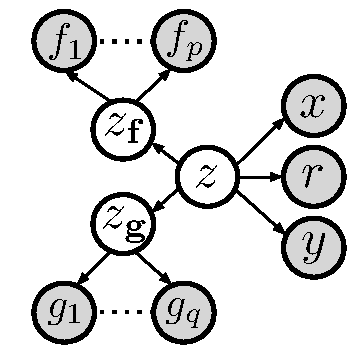
\includegraphics[width=0.6\fullwidth]{combined-topicmodel}}
\caption{ハイブリッド型のトピックモデル\cite{trieice:06:04}}
\label{fig:combined-topicmodel}
\end{figure}

文献\cite{trieice:06:04}では,アイテムの特徴$\bff$に加え,利用者の個人属性特徴や,利用意図などの特徴$\bfg=\paren{g_1,\ldots,g_q}$を加えた図\ref{fig:combined-topicmodel}のようなモデルを提案している.
これをまとめると次式のようになる.
\begin{multline*}
\pb{x,y,r,\bff,\bfg} =
 \pb{z}\pb{x|z}\pb{y|z}\pb{r|z}\\
\paren{\pb{z_\bff|z}\prod_i^p\pb{f_i|z_\bff}}
\paren{\pb{z_\bfg|z}\prod_j^q\pb{g_j|z_\bfg}}
\end{multline*}
%
このように,潜在変数を用いたトピックモデルには,推薦に関係するさまざまな要素を自在に導入できる柔軟性がある.
モデルを与えれば,EMアルゴリズムなどによりパラメータを学習できる.
いろいろなモデルの中から,集めたテストデータに,機械学習でのモデル選択の手法を適用して,最終的に利用するモデルを最終的に選べばよい.

もう一つの完全結合の手法として,関数モデルにカーネルを導入する\cite{icml:04:06}の方法を紹介する.
この方法では,順序回帰問題に帰着させてモデルを獲得する.利用者$x$がアイテム$y$を好む度合いを次の関数でモデル化する.
\[
f(x,y)=\sum_{(i,j)}w(i,j)K\paren{(x,y),(i,j)}
\]
ただし,$w(i,j)$は重みである.そして,しきい値$\theta_k$について$f(x,y)\in[\theta_{r-1},\theta_r)$を満たすなら,利用者$x$のアイテム$y$に与えた評価値は$r$と予測する.
この重み$w(x,y)$としきい値$\theta_k$は,順序回帰問題のためのパーセプトロン型の学習則であるPRankアルゴリズム\cite{nips:02:01}で獲得する.
そして,$K\paren{(x,y),(i,j)}$はカーネル\cite{jb:036:00}であり,協調と内容ベースフィルタリングを結合するときに中心的な役割を果たす.
この利用者$x$とアイテム$y$の対についてのカーネルは,適当な仮定のもと,利用者とアイテムそれぞれのカーネルの積となる.
\[
 K((x,y),(i,j))=K_X(x,i)K_Y(y,j)
\]
利用者については,$x=x'$なら$1$,でなければ$0$をとるカーネル,利用者の個人属性情報の特徴量$\bfg(x)$に基づくカーネル,利用者
$x$と$i$の間の\ref{sec:user-user}節の式\eqref{eq:glsim}の相関をとるカーネルなどを個々に求め,これらのカーネルの和を$K_X(x,x')$とする.
アイテムについても同様にカーネルを定義できる.
この方法では,カーネルを自由に設計できるので,いろいろな要因を考慮した推薦が可能である.
さらに,カーネルトリックが適用できるどのような関数モデルにも適用できるので,多様な応用が可能でもある.

\section{嗜好の予測手法の選択}
\label{sec:rsselect}
%@@@ アルゴリズムの最初のまとめの章に移動

嗜好の予測手法のまとめとして,予測手法の選択指針を,私見をまじえつつ列挙しておく.

最初に,協調フィルタリングか内容ベースフィルタリングかの選択について述べる.
\ref{sec:cfcbfcomp}節では,両方の手法の長所と短所について論じた.
これらのうち,内容ベースにとってはアイテム特徴のデータベースを構築し,維持できるかどうかが最大の制約である.
この構築・維持コストは,人手を要するため,一般に非常に高い.
もう一方の協調フィルタリングでは,嗜好データを収集できるかが大きな制約である.
利用者に負担をかけずにその嗜好パターンを巧妙に捉える暗黙的な収集方法か,利用者に評価付けしてもらうよい動機付けが必要になる.
これらの両方の制約を満たせるならば,それぞれの長所を生かしたハイブリッドがよいだろう.

\ref{sec:systemtarget}節の運用目的別では,概要推薦であれば,非個人化推薦である人気リストや,直接指定型の内容ベースとなり,利用者評価では,システム側は基本的に場を提供するだけで,予測手法は不要である.
関連アイテム推薦では,アイテム間型メモリベースの協調フィルタリングや,アイテムの特徴を用いて関連アイテムを見つけるのが一般的である.
通知サービスや緊密な個人化では,個人情報を蓄積していることが前提なので,協調フィルタリングや間接指定型の内容ベースが利用され,予測手法の役割が重要になる.

ここで,searchとexperienceいう推薦対象アイテムの種別\cite{ej:053}についてふれておこう.
searchアイテムとは,カタログの規格からの洞察によって,どれを購入するかを選択できるもので,実用品に多い.こうしたものには,基本的には直接指定型の内容ベースを利用する.
協調フィルタリングや間接指定型の内容ベースは,順位付けなどのために補助的に利用される.
後者のexperienceアイテムは,実際に試さないと判断できないもので,嗜好品などに多い.こうしたものでは,協調フィルタリングでセレンディピティを重視した推薦が有利となる.

次に,協調フィルタリング手法の中での選択について論じる.
まず最初に,どの手法も背後にいろいろな前提がある.
例えば,\ref{sec:timeseries}節の定期購読を対象とした方法は,推薦ごとに利用者が決定をする通常の推薦には適用できない.
各手法の前提に,推薦システムを適用しようとする対象が合っているかどうかは定性的に検証すべきである.
\ref{sec:memory-model}節で述べたように,データの更新が頻繁ならメモリベースが有利だが,そうでなければモデルベースが高速な推薦が可能である.
%文献\cite{uai:98:01}では,明示的な多段階評価ではメモリベースが,適合/不適合の二段階評価ではモデルベースが全般的に有利である.
%明確な証拠はないが,こうした傾向は一般に見られると考えを著者も支持する.
%二段階評価は,暗黙的に獲得した嗜好データが多く,未評価と不支持の区別ができない.
%これらを区別せずに不支持として処理するため,メモリベースは不利になる.
%一方,多段階評価ではモデルベースは推定すべきパラメータ数が増えるため,二段階評価に適している.
%もちろん,十分なサンプルが準備できるならば,モデルベースでも高精度な推定が可能である.

メモリベース法には,利用者間型とアイテム間があるが,予測精度よりも他の規準でどちらかを選択すべきだろう.
アイテムの更新が頻繁である場合や,セレンディピティなどについては利用者間型が有利だろう.
一方,一時的個人化をしたい場合や,利用者の入れ替わりが頻繁な場合にはアイテム間型が有利だろう.
%新規利用者に,特定のアイテム群について評価値を入力させる方法は,アイテム間型では無意味である.
%改良手法の中で,評価値平均を0にする正規化と,デフォルト投票は有効な場合が多いようなので,検証してみるとよいだろう.

%@@@ 履歴条件型・共起型のモデルの変更
次にモデルベース法について述べる.クラスタリングモデルは,非常におおまかな推薦しかできない.新規利用者を対象としたおおまかな推薦が主な利用法だろう.
他の要因を無視して,予測精度だけを重視するならば,行列分解を用いる関数モデルが,近年の研究では有利であるように著者は思う.
確率モデルは,多様な方法が提案されており,いろいろな状況に適応できる.
確率モデルの履歴条件型と共起型を比較すると,飽和モデルのパラメータ数はそれぞれ${|\calR|}^m-1$と$nm\abs{\calR}-1$となる.
よって履歴条件型は,評価値が多段階だったりアイテム数が増えたりすると極端に不利になりやすいが,利用者数には依存しないので,利用者は多いほど高精度のモデルが学習できる.
一方,共起型は評価値の段階数,アイテム数,および利用者数のいずれに対しても線形で,破綻しにくいといえる.
また,暗黙的な評価値で,未評価と否定的評価が区別できないときには共起型が有利である.
%実際には,飽和モデルではなく,グラフィカルモデルなどの手法でよりパラメータ数の少ない確率モデルを利用する.
時系列モデルは,成長に合わせて購入する製品が変わる子供用品など,時間に大きく依存する場合には有効である.ただし,時刻を考慮する分だけモデルは複雑なので,十分なデータは必要になる.
嗜好の揺らぎを考慮する手法も幾つか紹介した.嗜好データに揺らぎがあるかどうかは,\ref{sec:explicitrating}節で述べたように,時間をあけて同じ被験者から嗜好データを集め,整合性が低いかどうかで調べる.

%@@@ 推薦アルゴリズムの検証方法の章
あらゆる状況でうまく予測できるアルゴリズムは存在しないので,サンプルデータを収集して交差確認法で汎化誤差を実験的に求め,手法を比較したり,パラメータを調整する手続きは不可欠である.
調整パラメータ数が増えるアルゴリズムを使ったときには,予測精度の向上がわずかならば,パラメータ数の少ない方法を使っておくか,
\ref{sec:recomtype}節で述べたように,データを訓練・確認・テストに3分割した厳密な方法で検証することを薦める.


\part{推薦システムのその他の話題}
\label{part:topic}
%!TEX root =  main.tex
%!TEX encoding = UTF-8 Unicode
\chapter{プライバシー保護協調フィルタリング}
\label{sec:privacycf}

協調フィルタリングでは,標本利用者の嗜好データを収集する.このデータが,商品の購入履歴などであった場合は,これらの情報は利用者が秘匿したい個人情報となるであろう.
さらに,断片的な情報を集積することで,より重大な個人情報を得ることもできるようになってきている.
例えば,Sweeneyは,87\%のUS在住者が,性別,5桁郵便番号,生年月日の情報だけで一意に特定できることを示した\cite{misc:079}.
映画の評価について,掲示板発言と,これとはまた,独立した推薦システムの評価データのパターンの類似性から,匿名の利用者のIDの対応付けがかなりの割合でできるとの報告もある\cite{sigir:06:05}.
現在では,プライバシーは「個人が自らの情報を自分でコントロールできる権利」\cite{jjsai:06:05}を意味するようになり,ますます重視されるようになってきている.
一方,協調フィルタリングはこうした個人情報なしには実現できないので,これらの情報を収集する必要がある.

現状では,この個人情報の収集に伴う問題には,プライバシー・ポリシーを公開し,それを遵守することを誓約することで,社会的手段によって対処している.
これに対し,技術的手段によってこの問題に対処するのが\term{プライバシー保護協調フィルタリング}{privacy-preserving collaborative filtering}である.
プライバシー保護協調フィルタリングの技術は,\term{プライバシー保護データマイニング}{privacy-preserving data mining}\cite{eb:056:00,jjsai:09:01}と関連が深い.
これは,分散環境の各サイトに分割されて保持されているデータがあるとき,それら全てを集めたデータ集合に対するデータマイニング結果を,各サイト内のデータの内容を自分以外のサイトは秘密にしたまま計算する技術である.
この計算を実現するアプローチとしては暗号化\cite{lncs:00:04}とランダム化\cite{sigmod:00:03}とを使う方法がある.
プライバシー保護協調フィルタリングにおいても,この二つのアプローチがある.
これらを順に説明する.


\begin{figure}
\centering
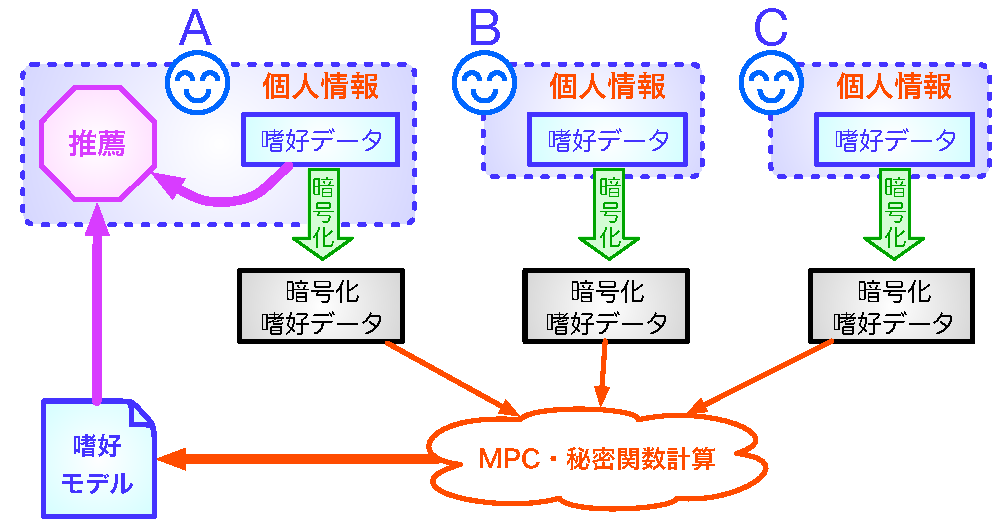
\includegraphics[width=0.96\fullwidth]{privacycf1.pdf}\\\smallskip
(a)~暗号化による方法\\\bigskip
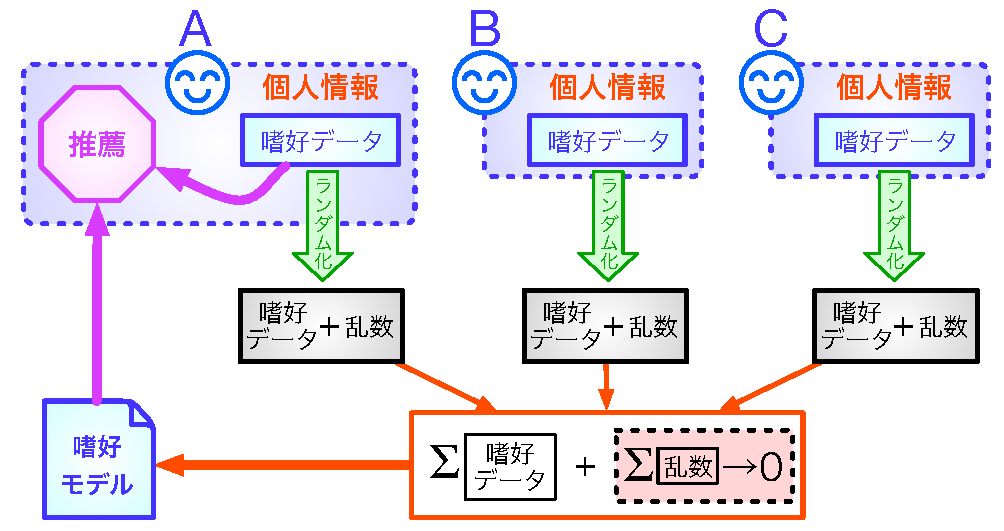
\includegraphics[width=0.96\fullwidth]{privacycf2.pdf}\\\smallskip
(b)ランダム化による方法
\caption{プライバシー保護協調フィルタリング}
\label{fig:privacycf}
\end{figure}

\section{暗号化による方法}

モデルベースの協調フィルタリングでは,標本利用者の嗜好データではなく,それらの規則性を表したモデルさえあれば推薦が可能である.
よって,嗜好データそのものを知らせることなくモデルが構築できれば,各利用者がどのような評価をしたかは秘匿できる.
また,メモリベースの協調フィルタリングでも,評価値行列を次元削減したものを公開すれば,個々のアイテムへの評価値は秘匿できる.
これを,データを暗号化したまま計算するという技術によって実現する.
この技術としては,ほとんどの計算が可能だが計算量は多い multiparty secure computation~\cite{misc:010}や,計算の種類ごとに専用の方法が必要だが高速に計算できる\term{秘密関数計算}{secure function evaluation}~\cite{kdde:02:03}がある.
\index{secure multiparty computation}

このアイデアに基づく枠組みを\ref{fig:privacycf}(a)に示す.
まず,標本利用者は自身の嗜好データを暗号化して推薦システムに渡す.
ここで,渡されたデータは暗号化されているため,個人情報は外部には漏れない.
これらの暗号化嗜好データに,秘密関数計算などの技術を適用して,暗号化された状態のモデルを獲得する.
最後に暗号化モデルを復号して目的の嗜好モデルを得る.
ここで,この嗜好モデルは標本利用者全般の嗜好の規則性の情報を表してはいるが,このモデルから個々の標本利用者の嗜好データ自体を復元することはできない.
よって,個人の評価情報は漏洩しない.
活動利用者は,自身の計算機上で,このモデルと自身の嗜好データから推薦を得ることができる.
モデルには,利用者間型メモリベースで次元縮約を使うもの\cite{ec:007}や,\ref{sec:funcmodel}の行列分解を使うもの\cite{sigir:02:01}などがある.

しかし,現状のプライバシー保護協調フィルタリングでは,社会的手段が補助的に必要となる.
計算結果が改竄されていないかを検証するには,半数以上の参加者は,個人情報を明かすほど信頼はできないが,計算の手続きは遵守する程度には信頼できるという semi-honest という前提が必要である.
しかし,この前提の技術的手段による保証は難しく,社会的手段によって保証しなければならない.
そのため,匿名で参加できるpeer-to-peerネットワークなどでの実現は難しい.
ソーシャル・ネットワークなど個人認証がなされるサービスでの推薦や,複数の企業が自身の顧客の情報を秘匿しつつ,共同して推薦をしたい場合などを想定すべきである.

\section{ランダム化による方法}

安全な計算は,暗号化はしているが,個人情報の真の値を外部に出している.
そうではなく,真の値ではない値を外部に出す方法が\term{ランダム化}{randomization}による方法(\ref{fig:privacycf}(b))である.

原理は単純で,平均値が0の正規分布や一様分布に従う乱数を加えてから,自分のデータを外部に出力する.
このとき,全参加者は同じ確率分布から独立にサンプリングした乱数を用いることが重要である.
ここで,全参加者の出力した値の総和や内積を求める.この値は,真の値の総和に,乱数の総和を加えたものになっている.
ここで乱数の総和は,元の分布の平均である$0$に漸近的に近づく.
よって,十分な数のデータがあれば,総和や内積が近似的に計算できる.
この手法によるプライバシー保護協調フィルタリングは\cite{icdm:03:01}などで提案されている.
この方法は,真の値は外部に出さなくて済む利点があるが,加える乱数の標準偏差が小さいと,真の値が近似的に予測できてしまうとか,厳密な値ではなく,近似値しか計算できないといった欠点がある.

%!TEX root =  main.tex
%!TEX encoding = UTF-8 Unicode
\chapter{サクラ攻撃}
\label{chap:shilling}

\begin{figure}
\centering
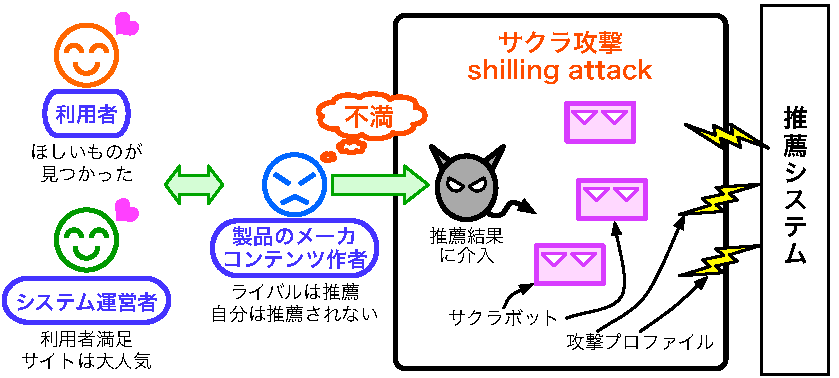
\includegraphics[width=0.96\linewidth]{shillingattack.pdf}
\caption{サクラ攻撃を行う動機}
\label{fig:shilling-motivation}
\end{figure}

推薦システムの効用について考えてみよう(図\ref{fig:shilling-motivation}).
利用者は知りたい情報を入手できるようになり,システムに満足するだろう.これにより,システムの運営者には,システムが利用が促進されるという利点がある.
では,利用者に推薦される製品や情報の提供者にとってはどうであろうか?
自身の製品の代わりに競合他社の製品が推薦されて欲しくないとか,たとえ自社の製品が推薦されいても,さらに推薦されるよう望んだりするだろう.
これらの要求は必ずしも満たされるとは限らないため,推薦結果を自身に有利にする目的で推薦システムに干渉することが行われ始めている.
具体的な事例は\cite{www:04:01}を参照されたい.

こうした行為の一つに\term{サクラ攻撃}{shilling attack}がある.
これは,\term{サクラボット}{shilling bot} と呼ばれるエージェントプログラムや,雇った人間に,自身に有利な推薦が他の利用者になされるように,推薦システムへ嗜好データを入力させるものである.
サクラ攻撃は,利用者にとっては不適切な推薦がなされるため望ましくない.運営者にとってもシステムへの信頼を失わせる行為であるため,サクラ攻撃は排除すべきものである.
サクラ攻撃の有効性の検証や,攻撃検出などの対策は,文献\cite{jacm:04:02,www:04:01}などによって研究が始められた.
サクラ攻撃全般についてのよいまとめとしては文献\cite{ieeem:07:07}がある.
以下,サクラ攻撃の構成要素,攻撃戦略の体系的な分類,攻撃への対策を紹介する.

\section{サクラ攻撃の基本}
\label{sec:shilling:basics}

サクラ攻撃の基本事項をまとめる.
攻撃意図とは,攻撃の実行者が推薦をどのように変化させたいかという目的である.
\begin{description}
 \item[販促攻撃 (push attack)] 本来なら推薦されないはずの,自社の製品などのアイテムを推薦されるようにする.
 \item[排除攻撃 (nuke attack)] 本来なら推薦されるはずの,他社の競合製品などのアイテムを推薦されないようにする.
 \item[攪乱攻撃 (random attack)] 予測精度を下げさせて,システムへの信頼を失わせる.
\end{description}
このうち前者二つの攻撃目的について研究がなされている.
こうした攻撃は,一部の限定された利用者やアイテムに対して集中的に行われる.

一般に,大量の情報,またシステムに密接な情報を利用した攻撃ほど効果的な攻撃が可能になる.
特に,利用者の嗜好データに完全にアクセスできると,検出はほぼ不可能である.
しかし,この種の情報は,プライバシー保護の観点からも秘匿されて管理されているため,攻撃者が合法的に入手するのは困難である.
比較的容易に合法的に入手できるデータとして,アイテムへの平均評価値がある.
これらのデータを公開しているシステムや,利用者そのものでなくても,コメントを付けている編集者や利用者の評価の平均値を出しているものは多い.
さらに映画におけるIMDB~\cite{url:021}のように,アイテムの評価サイトから,代替情報を別途入手できる場合もある.
また,推薦アルゴリズムごとに効果的な攻撃の作戦があるので,推薦に用いているアルゴリズムの情報も重要である.
一時的な推薦を,協調フィルタリングで行うには,アイテム間型のメモリベース手法が多用されるといったことを用いて,この情報もある程度推定できる.

サクラ攻撃の効果は次のような指標によって測る.
\begin{description}
\item[予測シフト (Prediction Shift)] 攻撃の前後での,予測評価値の変化の全標的アイテム(後述)と全利用者についての平均.予測評価値自体がどれくらい攪乱されたかを測るための指標である.
\item[ExpTopN(Expected Top-N Occupancy)] 上位N個の推薦アイテムに標的アイテムが含まれる個数の,全利用者についての期待値.評価値が変化しても,アイテムの順位に影響するとは限らないので,実際の推薦リストの変化を測るための指標である.
\end{description}

\section{サクラ攻撃の種類}
\label{sec:shilling:tactics}

\begin{figure}
\centering
\subcaptionbox{標的アイテムのみ\label{fig:attackprofile:a}}%
{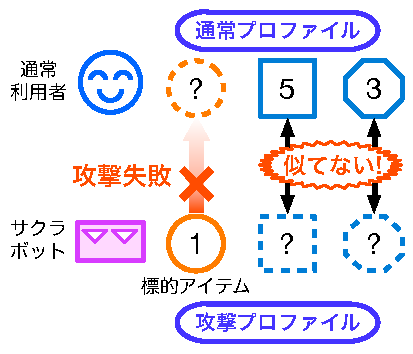
\includegraphics[width=0.6\fullwidth]{attackprofile1.pdf}}\\\bigskip
\subcaptionbox{標的アイテム+詰め物アイテム\label{fig:attackprofile:b}}%
{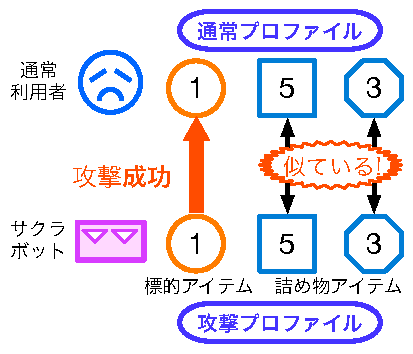
\includegraphics[width=0.6\fullwidth]{attackprofile2.pdf}}
\caption{攻撃プロファイル}
\label{fig:attackprofile}
\end{figure}

サクラ攻撃をどのように行うかについて述べる\cite{www:04:01}.
図\ref{fig:attackprofile}は,排除攻撃の様子を示した.
まず,図\ref{fig:attackprofile:a}に注目されたい.
上側は,通常利用者の嗜好データ(通常プロファイル)を示した.
この通常利用者に推薦されるアイテムを,サクラ攻撃によって変えたいとする.
一方,下側は,仮想利用者であるサクラボットが推薦システムに入力する嗜好データで,攻撃プロファイル (attack profile) と呼ぶ.
図中には,丸,四角,八角で示した三つのアイテムがあり,各プロファイル中では,これらのアイテムは5段階で評価されている.
「5」が最高評価,「1」が最低評価,そして「?」が未評価を示している.
この中で,丸で示したアイテムは,排除したい競合製品を表し,これを標的アイテム (target item) と呼ぶ.
通常利用者はこの標的アイテムを未評価で,今からこの利用者の標的アイテムへの評価値を予測するとしよう.

このとき,標的アイテムを推薦されないようにするには図\ref{fig:attackprofile:a}のように,サクラボットは標的アイテムに最低の評価「1」を与えさえすれば良さそうである.
しかし,この攻撃は失敗する.多くのサクラボットが悪い評価を与えることで,このアイテムへの平均的な評価は確かに低下する.
だが,協調フィルタリングでは,嗜好パターンが似ている利用者を参考に推薦することを思いだされたい.
この利用者の通常プロファイルでは,標的アイテム以外の四角や八角のアイテムも評価されている.
一方,攻撃プロファイルでは,丸の標的アイテムのみが評価され,それ以外の四角や八角のアイテムは全て未評価である.
そのため,通常プロファイルと攻撃プロファイルは似ていないと判定され,サクラボットとこの利用者の嗜好パターンは違うとみなされる.そのため,標的アイテムの評価は通常利用者の推薦には反映されず,攻撃は失敗する.

そこで,他の利用者の嗜好パターンに攻撃プロファイルを似せるため,図\ref{fig:attackprofile:b}のように,標的アイテム以外の四角や八角のアイテム群にも評価値を与える.
これらのアイテムを詰め物アイテム (filler item) と呼ぶ.
これらの,詰め物アイテムへの評価が通常利用者のそれと類似していれば,通常プロファイルと攻撃プロファイルとは類似していると判断される.
すると,攻撃プロファイルの標的アイテムへの評価は,通常利用者の推薦に影響し,攻撃は成功する.
しかし,通常利用者の嗜好データは入手できない.
よって,詰め物アイテムの評価値は,通常利用者の,一般的な評価の傾向に基づいて与える.
この与え方の違いによって,次のような攻撃方法がある.
\begin{description}
\item[サンプリング攻撃 (sampling attack)]
詰め物アイテムに,システムのデータベースからサンプリングしてきた評価値を与える.統計的手法では検出は不可能と言って良いが,システム内のデータベースの情報の入手は非常に困難である.
\item[ランダム攻撃 (random attack)]
ランダムな評価値を,詰め物アイテムに与える\cite{www:04:01}.必要な情報はないが,あまり効果はなく発覚し易い.
\item[人気商品攻撃 (bandwagon attack)]
良く売れている人気商品の評価は高いことが多く,また多くの利用者が評価している.
のことを利用し,人気商品に高い評価値を与えて,攻撃プロファイルの他の利用者への類似性を高める\cite{jacm:04:02}.
\item[平均攻撃 (average attack)]
詰め物アイテムに,それらのアイテムへの評価値の平均値を与える\cite{www:04:01}.
アイテムへの平均評価値は入手が比較的容易だが,利用者間型のメモリベース手法には効果的である.
一方,アイテム間型では,予測シフトで評価すると確かに評価値には影響するが,推薦リスト中でのアイテムの順位を変えるまでにはいたらず, ExpTopNへの影響は限定的である.
\item[探査攻撃 (probe attack)]
ダミー利用者を作り,その利用者に推薦されたアイテムの予測評価値を詰め物アイテムへの評価値とする\cite{ieeem:07:07}.
ダミー利用者と類似した嗜好の利用者にのみ有効な攻撃である.
\item[セグメント攻撃 (segment attack)]
映画のジャンルなど,アイテムの分類情報が利用できる場合の販促攻撃に用いる\cite{icdm:05:06}.
標的アイテムと同じセグメント(分類カテゴリ)のアイテムには,高い評価を与える.
同じセグメントのアイテムには,同じような評価がなされやすいという傾向を使う.
アイテム間型のメモリベースに対して有効な攻撃である.
\item[愛憎攻撃 (love/hate attack)]
排除攻撃専用の手法.標的アイテムには最低の評価を,詰め物アイテムには最高の評価を与える\cite{kdd:06:01}.
単純な攻撃だがアイテム間型と利用者間型のどちらのメモリベース手法についても効果がある.
\end{description}
%他の利用者がまだあまり評価していない,新規のアイテムについては,サクラ攻撃には特に脆弱である.
%現在のところ,モデルベース型の協調フィルタリングについては,まだこれらの攻撃の効果は研究が進んでいない.

\section{サクラ攻撃に対する防御}
\label{sec:shilling:defence}

作為的な利用者の評価に影響されて,協調フィルタリングが不適切な推薦をしたとしよう.
そして,他の利用者がその推薦に従ったとしても,その後,作為のない評価をするので,自律的にこうした攻撃は無力化されるとも考えられていた.
しかし,Cosleyら\cite{sigchi:03:02}はこれに対して否定的な調査結果を報告している.
以前に評価したことのあるアイテムについて,以前と同じ,1段階良い,1段階悪いの3種類のものを「予測評価」と偽って利用者に提示した.
すると,作為的にずらした方向に,アイテムへの利用者の評価が変化した.
さらに,未評価のアイテムについて,アルゴリズムができるだけ正確に予測した評価,それより1段階良い/悪い評価を利用者に提示すると,やはり,同様の傾向がみられた.
このように,心理学における同調 (conformity)~\cite{jb:026:00}と類似した,周りの意見に利用者の意見が『引きずられる』現象が報告されている.
そのため,サクラ攻撃に対して推薦システムは自律的に回復することはできず,攻撃を検出して排除する必要がある.

サクラ攻撃は,サンプリング攻撃以外は,真のデータベースの評価値分布と,攻撃プロファイルとの統計的な分布の差をはずれ値検出の技術によって見つけることで検出する.
文献\cite{sigir:06:01}の方法は,最も基本的なもので,モデルから予測される評価値と,実際の評価値の差が標準偏差に対して十分に大きければ攻撃とみなす.
ランダム攻撃は比較的に容易に検出できるが,平均攻撃では失敗することも多い.
また,サクラボットが評価するアイテム数が少ない場合や,標的アイテムが多い場合は検出が困難になると報告している.
文献\cite{kdd:06:01}では,アイテムに対する平均的な評価からの乖離を,被評価数などで加重した統計量や,ボットの攻撃は多数のアイテムに対して行われることを利用した統計量を提案している.
加えて,平均攻撃など特定の攻撃に対する検出方法も検討している.
その他,攻撃が特定の時期にまとまって行われることが多いことを利用し,時系列中での検出を試みる研究\cite{kdd:06:03}もある.
これは,あるアイテムについての評価値を,一定間隔の期間ごとに分ける.
そして,各期間内の評価値の平均やエントロピーが異常値になることを検定により検出する.
文献\cite{sigir:08:04}はサクラ攻撃に対して頑健な,行列分解を用いた推薦アルゴリズムを提案している.
この方法では,評価値行列を因子に分解するときに,利用者側の因子はそのまま計算するが,評価パターンが他の利用者と大きく異なっている疑わしい利用者の因子を利用せずにアイテム側の因子を計算する.

%!TEX root =  main.tex
%!TEX encoding = UTF-8 Unicode
\chapter{推薦システムのその他の問題や視点}
\label{chap:othertopic}

その他の視点に関する研究をまとめて述べる.

\section{対話型システム}
\label{sec:interactive}

これまでの推薦システムは,過去に入力された嗜好データに基づいて利用者の嗜好を予測し,一度だけ推薦の提示を行う.
だが,利用者がその推薦に満足できない場合がある.
そうした場合に,活動利用者からフィードバックを得て,その情報用いてより適切な推薦をする対話的な推薦も研究されている.
フィードバックは,アイテムへの評価値を返すアイテムレベルと,アイテムの特徴を指定する特徴レベルとに分けられる.これらを順に紹介する.

\subsection{アイテムレベルのフィードバック}

機械学習のクラス分類の訓練事例では,ラベル付けされている事例の特徴ベクトルは受動的に決められているのが一般的である.
そうではなく,能動的に都合のよい特徴ベクトルをもつような事例を指定すると,それに対するラベル情報が得られる状況を扱うのが能動学習\cite{jb:035:00}である.
この枠組みを導入し,推薦の予測精度が不十分だった場合に,推薦を改善するのに役立つであろうアイテムを利用者に評価してもらうことが考えられる.
ではどのアイテムを評価させるのがよいだろうか?
直観的に,利用者によって評価にばらつきがあり,好みの分かれるアイテムを評価してもらうのはよいだろう.
このように,教師情報を得るデータを能動的に選択する機械学習の枠組みを\term{能動学習}{active learning}という.
この枠組みに基づいて,他の利用者の評価値の分散やエントロピーが大きなアイテムを選ぶ方法が提案されている\cite{ec:033}.
文献\cite{uai:03:02}では,アイテム選択の尺度として,期待情報価値 (expected value of information; EVOI) を提案している.
まず,現在の嗜好データで予測したとき,期待的に最も良い評価値は,全未評価アイテム上での,期待評価値の最大値である.
ここで,未評価アイテムの一つ$x_q$に対する評価値を利用者から得ると,この最大期待評価値は変化するはずである.
だが,どのような評価値を利用者が返すかは分からないので,評価後の最大期待評価値の,評価値定義域$\calR$上の期待値を考える.
この期待値から,評価前の最大期待評価値を引いた値をEVOIとする.
すると,EVOIは,利用者からアイテム$x_q$に対する評価値を得たことによる,最大期待評価値が改善する量を表す.
よって,このEVOIを最大にする未評価アイテムを活動利用者に評価してもらえばよい.
だが,実際には計算量が多いため,このEVOIの値の代わりにその上限を計算して代用する.
その他,候補アイテムの評価値が予測どおりであったときと,それとは若干ずれた値であったときの,他の未評価アイテムの予測評価値の変化の大きさが大きいアイテムを選ぶ方法も提案されている\cite{trjsai:07:06}.
この能動的評価の問題点は,利用者が任意のアイテムをすぐに評価でなければ適用できないことである.
例えば,音楽であればその場で聞かせて評価させることができるが,映画や書籍の場合では難しい.

純粋な協調フィルタリングでは,コンテキストの情報(\ref{sec:featuredata})を利用できない.
また,コンテキスト自体を特徴として明示することが困難な場合がある.
そこで,文献\cite{ej:051}は嗜好データを長期と短期のプロファイルに分けて考える手法を提案している.
長期プロファイルとは,現在の推薦のセッションより以前に入力された嗜好データで,利用者の基礎となる嗜好パターンを表しているとみなす.
一方,現在のセッションで提示した推薦リスト中のアイテムに対する嗜好データが短期プロファイルで,現在のコンテキストでの嗜好を示しているとみなす.
フィードバックは,目的のアイテムに近いものや,全く当てはまらないものを利用者に指定させる.
予測には利用者間型のメモリベース法(\ref{sec:user-user})に基づく.
長期プロファイルに基づいて活動利用者と標本利用者の間の類似度を計算する点は同じである.
しかし,フィードバックで肯定的だったアイテムを好み,そうでないものを嫌うような標本利用者を重視するように,標本利用者を重み付けする.
このようにして,短期プロファイルに暗黙的に示されたコンテキストを反映する推薦が実現される.

文献\cite{ijcai:03:04}は,対話的な推薦で,候補アイテムが適切に絞り込まれているかを検証する方法を提案している.
アイデアは非常に簡潔で,前回の推薦で肯定的なフィードバックが与えられたアイテムを,次回の推薦リストに混ぜておく.
もし,その混ぜておいたそのアイテムが再び選択されるようならば,絞り込みは適切でなかったと判断し,他の方向からの絞り込みに変える.
そうでなければ,同じ方向で絞り込みを続ける.

\subsection{特徴レベルのフィードバック}

特徴レベルのフィードバックは,アイテムの特徴を扱うため,内容ベースフィルタリングが対象となる.
この種のフィードバックでは,推薦されたアイテムを見て,アイテムの望ましい性質を利用者が示す.
例えば,パソコンではメモリが1GB以上といった,アイテムの特徴に対する条件の精細化をする.
\ref{sec:cbf}で述べたように,内容ベースの推薦は情報検索と類似しているので,情報検索でフィードバッ
クを扱う手法が,内容ベースの推薦に応用できる.
情報検索では,検索質問と関連する語を利用者に提示し,利用者がそれを選択することで,検索質問拡張を実現するものがある.
これと同様の手法が,推薦システムでも利用されている\cite{ec:024}.

その他,文献\cite{ej:049}では,\ref{sec:explanation}のように,説明を導入してより円滑に対話的な推薦を行うことを提案している.
ある特徴レベルフィードバックを利用者が返すと,次の推薦で候補の数や内容がどのように変わるのかを簡潔に説明し,より適切なフィードバックを得られるようにしている.

\section{標本利用者の選別}
\label{sec:sampleselection}

協調フィルタリングでは,他の標本利用者の意見を参照する.
このとき,嗜好が似ているだけでなく,該当分野に詳しい利用者の意見を参照する方がよいだろう.
こうした試みは,協調フィルタリングが自動化される以前からある\cite{macm:97:04}.

自動化された協調フィルタリングで,標本利用者を目的に応じて選別するアイデアには次のようなものがある.
%
ある標本利用者の嗜好データから,いろいろな活動利用者の評価値を予測する.
このとき,より多くの活動利用者の評価値を正確に予測できたとすれば,その標本利用者は他の活動利用者の評価値予測にも有用だろう.
文献\cite{ec:027}は,このアイデアに基づいた標本利用者の重み付けを提案している.
%
文献\cite{tjsai:04:09}では,各利用者が個別に文書レポジトリを所有しており,そのレポジトリは公開されている状況を想定する.
各文献を特徴ベクトルで表現し,活動利用者の評価とある標本利用者のそれが類似しているとき,その文献に関連した特徴に関して,その標本利用者は信頼できると考える.
そして,それと同じ特徴をもつ文献に対する評価では,その標本利用者の意見を重視する.
%
あるカテゴリのアイテムを,より多く評価している利用者は,そのカテゴリのアイテムについて詳しいと仮定してよいだろう.
このアイデアに基づき,文献\cite{ieeem:07:01}では,評価値を予測しようとしている目標アイテムと同じカテゴリのアイテムを多数評価している標本利用者の意見を重視することを提案している.

\section{推薦システムの運用}
\label{sec:rsysmanagement}

その他,推薦システムの運用に関係する問題についてまとめておく.
推薦システムを含めたフィルタリング技術の法的側面からの問題点を述べた解説としては\cite{jj:020}がある.
著名な推薦システムの内部アルゴリズムを概説した文献を挙げておく:オンライン小売りサイトAmazon.com\cite{ieeem:03:01},ニュースの要約サイトGoogle News\cite{www:07:01},学術文献検索サイトCiteSeer\cite{ieeem:99:02},推薦機能付きセットトップボックスTiVo\cite{kdd:04:01}.
稼働中のシステムの運用に関する情報として,書籍販売サイトbk1での推薦エンジンAwarenessNet\cite{jipsj:07:02}や,携帯向け映画推薦システムのストリートキャッチ方式によるアンケート調査\cite{trjsai:07:05}の結果などがある.

次に,推薦システムに関連の,マーケティング分野の研究について述べる.
まず,簡単な市場モデルを示した研究を挙げる.
文献\cite{ec:030}では,推薦システムが顧客の購入行動に影響を与え,市場の寡占化が生じるかを2個のアイテムがある市場の数理モデルで論じた.
購入したことを肯定的,購入しないことを否定的な評価としたとき,購入されたアイテムは推薦されやすくなり,寡占化がすすむ場合が多い.
そうならないのは,顧客が推薦を受ける以前は一方のアイテムを強く好んでいるが,推薦にも影響されやすいという状況だけに限られる.
文献\cite{ec:031}では,1回目に一方の店で購入すると推薦を受けられるが,他方の店で購入すると受けられないモデルの均衡状態を求めている.
このモデルで,推薦を受けられることの付加的な価値が,二つの店舗のシェアや顧客が購入するアイテムに与える影響を論じている.
推薦の正確さと,好みの方の商品を選択することが顧客にとってどれくらい重要であるかによって,4種類の異なる均衡状態があることを示している.

次に,推薦が顧客の意志決定に与える影響をアンケート調査した研究を示す.
文献\cite{ej:053}では,仕様だけで好みの判断ができるsearch型の商品群と,試さないと判断できないexperience型の違いについて調査し,experience型の商品群の方がより推薦に従うと報告している.
他の顧客の推薦より,推薦システムは信頼されていないにもかかわらず,実際の影響は推薦システムの方が強かったとも報告している.
また,販売業者から独立した組織の推薦であるかどうかは,信頼性や意志決定に影響しないことを報告している.
顧客はまだ知らないアイテムを推薦するとき,同時に提示する情報の影響について\cite{ej:054}は報告している.
顧客が好きなアイテムを同じ画面で共に示すと,知らないアイテムも同様にみなされて,好まれる.だが,この効果は,別画面に表示するだけで失われてしまう.
知らないアイテムに固有の情報与える(サンプル曲を聴かせるなど)と,差異が意識され,知らない推薦への魅力が下がるとも報告している.
なお,これらは,実際のシステムの推薦ではなく,推薦システムからの出力であることにして被験者に示した場合の調査結果である.

推薦システムによって,利用者の嗜好を逆転さえできることは,上記のような研究に加え\cite{sigchi:03:02}でも指摘されている.
だが,こうした行為を長期的に継続したときの影響は調査されていない.
著者は,推薦システムは\cite{dmkd:01:01}にもあるように販売側ではなく,顧客側に立つことは必要な条件だと考えている.
なぜなら,こうした利用者の嗜好のねじ曲げは,長期的には,推薦システムへの信頼を損なう危険が多いだろう.
こうしたことをせず,利用者の意向に沿うことに徹しても\cite{dmkd:01:01}にあるような三つの効用があるだろう.
第1に,顧客が真に好むものを積極的に提示することで,閲覧者を購入者に変える.
第2に関連商品を推薦してcross-sellを増加させる.最後に,顧客側の推薦を続けることによって長期的な顧客ロイヤリティを構築する.
推薦システムは,どんなに売れない商品を売ってしまう魔法の杖ではなく,逆に売れ筋商品の寡占を加速する場合もあることは意識しておくべきだろう.

\subsection{推薦の品質}
\label{sec:openproblem:quality}

予測精度以外の規準も考慮した推薦の品質\cite{sigchi:06:01}に関する研究を紹介する.

予測精度以外の評価指標の多様な規準の必要性は\cite{sigchi:06:02}などで指摘されている.
こうした基準には,アイテムの特徴\cite{www:05:01}や,単純な予測器\cite{trjsai:07:03} を用いた意外性の規準がある.
また,全利用者について推薦されるアイテムの種類の分布のGini係数を用いて推薦の多様性の評価する\cite{ec:030}も,アイテム集合全体を評価する点で興味深い.
現在は推薦するアイテムを個々に判断しているが,推薦リスト全体で最適化することを今後は重視してゆくべきだろう\cite{sigchi:06:01}.

データ入力段階では,利用者の要求をうまく獲得することが重要だろう.
まず,好きかどうかだけではなく,複数の評価項目について質問することで,どういう点で良かったのかを知る方法がある.
例えば,映画について,全体評価の他,脚本や配役などの評価も利用する\cite{ieeem:07:02}や,好みに加えて知っているかどうかも尋ねる\cite{trieice:07:03}などの研究がある.
暗黙的な獲得でも,閲覧,サンプル視聴,購入の行動を区別する\cite{ieeem:07:01}などの研究もある.
効果的な評価項目について検討する余地は広い.

嗜好の予測段階について述べる.
個人ではなく複数の利用者から構成されるグループに対する\term{グループ推薦}{group recommendation}がある\cite{ec:032,jc:011,misc:014,misc:015,misc:016}.
全利用者に対して平均的によい推薦や,だれにもあまり嫌われないような推薦など,いろいろな選択肢が考えられる.


\part{まとめ}
\label{part:conclusion}
%!TEX root =  main.tex
%!TEX encoding = UTF-8 Unicode
\chapter{参考資料の紹介}
\label{chap:reference}

推薦システムについてさらに知るには以下のような資料がある.

\section{代表的な文献,解説記事,および書籍}
\label{sec:reference-paper}

\subsection{英語}

\begin{description}[style=nextline]
\singlespacing
\item[Using Collaborative Filtering to Weave an Information Tapestry (1992)]
手動での検索ではあるが,初めて ``collaborative filtering'' の概念を提案した\cite{macm:92:01}
\item[GroupLens: An Open Architecture for Collaborative Filtering of Netnews (1994) と Social Information Filtering: Algorithms for Automating ``Word of Mouth'' (1995)]
現在の推薦システムに繋がる,最初の自動化した協調フィルタリングによる推薦システムであるGroupLens\cite{cscw:94:01}とRingo\cite{sigchi:95:02}
\item[Recommender Systems (1997)]
『推薦システム』という用語を定着させたCommunications of ACMの特集記事\cite{macm:97:01}
\item[Empirical Analysis of Predictive Algorithms for Collaborative Filtering (1998)]
初期の推薦アルゴリズムのサーベイと予測精度の比較\cite{uai:98:01}
\item[E-Commerce Recommendation Applications (2001)]
電子商取引サイトでの推薦システムの運用について述べた初期の文献ではあるが,ここで指摘された多くの考えは現在においても示唆に富んでいる\cite{dmkd:01:01}
\item[Evaluating Collaborative Filtering Recommender Systems (2004)]
推薦システムの評価について「良い推薦とは」ということに深い考察がなされている\cite{jacm:04:01}
\item[Toward the Next Generation of Recommender Systems: A Survey of the State-of-the-Art and Possible Extensions (2005)]
推薦システムの基本的なアルゴリズムを俯瞰し,拡張的な推薦タスクに言及\cite{ieeet:05:01}
\item[Attacks and Remedies in Collaborative Recommendation (2007)]
サクラ攻撃全般について概要を知るのによい\cite{ieeem:07:07}
\item[A Survey of Accuracy Evaluation Metrics of Recommendation Tasks (2009)]
推薦のタスクごとに適切な評価尺度を選ぶべきことを実験的に示した\cite{jmlr:09:01}
\end{description}

\subsection{日本語}

\begin{description}[style=nextline]
\singlespacing
\item[情報推薦・情報フィルタリングのためのユーザプロファイリング技術 (2004)]
嗜好データの収集全般についてまとめている\cite{jjsai:04:05}
\item[特集『情報のフィルタリング』(2006)]
有害情報のフィルタリングと表現の自由など法的観点から,推薦システムの概要まで情報フィルタリングについて幅広く扱う\cite{jmisc:013}
\item[特集『利用者の好みをとらえ活かす -- 嗜好抽出技術の最前線 --』]
推薦システム全般を簡潔にまとめた\cite{jipsj:07:01}他いくつかの解説記事を含む\cite{jmisc:014}
\item[推薦システムのアルゴリズム (2007--2008)]
本稿はこの拙著に訂正・加筆を行ったものである\cite{jpublist:076,jpublist:081,jpublist:083}
\item[情報推薦システム入門 --- 理論と実践]
ややヒューマン・コンピュータ・インターフェースよりの解説\cite{jb:047:00}
\end{description}

\section{チュートリアル講演}
\label{sec:reference-tutorial}

国際会議などで行われたチュートリアルを紹介する.
\begin{itemize}
\item Grouplens法とインターフェース関係\cite{sigchi:03:01}
\item 予測精度以外に考慮すべき多様性などの要素\cite{sigchi:06:01,sigchi:06:02}
\item 推薦システムでユーザインターフェースがはたす役割\cite{misc:029}
\item 推薦システムの評価\cite{misc:074}
\item 推薦システムとWebコンテンツ最適化の高度なアルゴリズム\cite{misc:046}
\item フィルターバブル問題に対するパネル\cite{recsys:11:02}
\item 推薦と情報検索の多様性\cite{misc:033}
\item ソーシャル推薦\cite{misc:027}
\item 利用者インタフェースの評価\cite{misc:030}
\item 推薦システムのABテストなど実地検証\cite{misc:060}
\item 推薦システム全般\cite{misc:087}
\end{itemize}

\section{Webサイト}
\label{sec:reference-www}

推薦システムに関連するWebサイトを紹介する
\begin{description}
\item{ACM Recommender Systems}
2007年から始まった推薦システムの国際会議\cite{url:023}
\item[ACM RecSysWiki]
国際会議Recommender Systemsのコミュニティにより運営されているWiki\cite{url:024}
\item[GroupLens Research Lab.]
MovieLensの実験システム,プロジェクトの参考文献,代表的なテストデータなどを参照できる\cite{url:012}
\item[Netflix Prize]
オンラインビデオ配信のNetflix社が100万ドルの賞金をかけて2006〜2011年の間に行ったコンペティションで,推薦の予測精度の研究に貢献した\cite{url:022}
\end{description}

\section{テスト用データ}
\label{sec:reference-data}

アルゴリズムを検証するために利用できるベンチマークデータを紹介する.
なお,推薦システム研究の初期によく利用された,映画評価データEachMovieやNetflixのコンペティションのデータなどもあるが,現在は配布が停止されているので,これを利用するのは避けた方がよいだろう.

\begin{description}
\item[Movielens]
映画推薦システムMovieLens(最も良く使われているベンチマーク)\\
\url{http://grouplens.org/datasets/movielens/}
\item[SUSHI Preference Data Sets]
著者が収集した寿司に対する嗜好データ,順位法と採点法の両方の評価\\
\url{http://www.kamishima.net/sushi/}
\item{Jester}
アメリカンジョークの推薦,評価スケールが100段階なのが特徴的\\
\url{http://www.ieor.berkeley.edu/~goldberg/jester-data/}
\item[BookCrossing]
書籍コミュニティサイト\\
\url{http://www2.informatik.uni-freiburg.de/~cziegler/BX/}
\item[Cuban cigers]
葉巻販売サイトの商品の閲覧と購入,サイトの閲覧行動\\
\url{http://isl.ifit.uni-klu.ac.at/}
\item[Audioscrobbler]
現在は Last.fm の一部となったAudioscrobblerの音楽データ\\
\url{http://www-etud.iro.umontreal.ca/~bergstrj/audioscrobbler_data.html}
\item[Flixster]
M.~Jammali が収集した,アイテムの評価に加えて,利用者間の信頼関係データを含むソーシャル推薦用\\
\url{http://www.sfu.ca/~sja25/datasets/}
\item[BibSonomy]
論文に関するソーシャルブックマークサイト\\
\url{http://www.kde.cs.uni-kassel.de/bibsonomy/dumps}
\item[MovieTweetings]
Twitterのツイートから映画の評価データを収集したもの\\
\url{https://github.com/sidooms/MovieTweetings}
\item[WikiLens]
タグ・評価付きのWikiのデータ\\
\url{http://grouplens.org/datasets/wikilens/}
\item[HetRec 2011]
RecSys2011の併設ワークショップでのデータ,評価の他に追加的な情報がありコンテキスト考慮型推薦などの実験に\\
\url{http://grouplens.org/datasets/hetrec-2011/}
\item[Yelp]
商品の評価サイト\\
\url{http://www.yelp.com/dataset_challenge/}
\end{description}

\section{ソフトウェア}
\label{sec:reference-software}

主なオープンソースの推薦システム
\begin{description}
\item[LensKit]
Grouplens研究グループが実装している\\
\url{http://lenskit.grouplens.org/}
\item[MyMediaLite]
Microsoft社の .NET 環境下で動作\\
\url{http://mymedialite.net/}
\item[GraphLab]
線形代数のライブラリだが,行列分解型の推薦アルゴリズムを多く実装している\\
\url{http://graphlab.org}
\item[Mahaut] MapReduce上で動作する大規模用\\
\url{http://mahout.apache.org/}
\end{description}


%!TEX root =  main.tex
%!TEX encoding = UTF-8 Unicode





% privacy
\nocite{kdd:09:01} % 差分プライバシのCF
\nocite{misc:003} % 差分プライバシの基本文献

% social recommendation
\nocite{ec:041}

% popularity bias, diversity
\nocite{misc:011} % PRPの基本文献
\nocite{ej:055}
\nocite{kdd:08:04}
\nocite{recsys:10:01}
\nocite{sigchi:08:01} % bandwagon effect
\nocite{url:005} % LongTailの基本文献

% evaluation
\nocite{etr:008} % ABテストで利用者に悪い影響が残る

% memory-based
\nocite{icdm:07:01} % 近隣法のバイアスとか

% web content optimization
\nocite{jml:02:03} % UCB1
\nocite{icdm:09:01}
\nocite{icml:99:02}
\nocite{www:10:01}

% RBM
\nocite{icml:07:05}

% matrix factorization
\nocite{kdd:08:05}
\nocite{kdd:09:02} % 時間付き
\nocite{kdd:09:03} % テンソル分解,タグ推薦
\nocite{misc:012} % 欠損の考慮
\nocite{url:009} % 確率的勾配降下

% preference elicitation
\nocite{recsys:11:01}


% ===== Back Matter =====
\backmatter


% ---- Acknowledgements ----
%\medskip
%\noindent\small\textbf{謝辞}:\ 
%みんなありがとう

% ---- Bibliography ----
\singlespacing
\small
\bibliographystyle{jsai}
\bibliography{ebib,epublist,emisc,jbib,jpublist,jmisc}

% --- Indexes ---
\pagestyle{empty}
\printindex

\end{document}
